\documentclass[12pt]{report} % Longer texts should use report, and this defines the letter size as 12pt

% PACKAGES -------------------------------------------------------------------------------------

% Layout
\usepackage[utf8]{inputenc} % Defines the encoding as utf-8
\usepackage{graphicx} % Required for inserting images
\usepackage[english]{babel} % English language package
\usepackage[a4paper,top=2.5cm,bottom=2.5cm,left=2.5cm,right=2.5cm,marginparwidth=1.75cm]{geometry}
\usepackage[autostyle]{csquotes} % For using block-quotes
\usepackage{float} % Used to keep tables and figures in place

% Text
\usepackage[colorlinks=true, allcolors=black]{hyperref} % Keeps hyperlinks black
\usepackage{lettrine} % This makes it possible to use large first letter for new chapters
\usepackage{lmodern} % This package must me useed to ensure that the lettrine package works as it is supposed to (It is a font that is scaleable, unlike the the default one)
\usepackage{amsmath} % Required for maths
\usepackage{amsfonts} % Required for checkmark
\usepackage{dcolumn} % Used for making decimal-centred columns
\usepackage{anyfontsize} % Used to change fontsize (mainly for tables)

% Citations
\usepackage[autostyle]{csquotes} % For using block-quotes
\usepackage{natbib} % Required for citation
\usepackage[nottoc]{tocbibind} % Package to add bibliography to the table of contents

% Tables
\usepackage{booktabs} % CHECK WHAT THIS DOES, it might be for getting the tables working correctly
\usepackage{tabularx} % For making tables fit the page
\usepackage{array} % For aligning text in the cells
\usepackage[table]{xcolor} % For colouring tables
\usepackage{ragged2e} % Provides \justifying
\usepackage{tabularray} % To display datasummary tables
\usepackage{codehigh} % Highlights code, idk. 
\usepackage{makecell} % To enable line-break in table cells
\usepackage{longtable} % Used to make multi-page tables

% Infographics
\usepackage{tikz} % For making infographic boxes and arrows
\usepackage{circuitikz} % Tikz when using figure maker

% CONFIGURATIONS -------------------------------------------------------------------------------

% Tikz
\usetikzlibrary{arrows.meta,bending,positioning,shapes.geometric}

% Citations
\bibliographystyle{chicago} % Sets citation style to chicago
\setcitestyle{aysep={}} % Removes comma between author and year for in-text citations

% Lettrine settings
\renewcommand*{\DefaultLoversize}{0.0}
%%%

% Datasummary table commands
\UseTblrLibrary{booktabs}
\UseTblrLibrary{siunitx}
\newcommand{\tinytableTabularrayUnderline}[1]{\underline{#1}}
\newcommand{\tinytableTabularrayStrikeout}[1]{\sout{#1}}
\NewTableCommand{\tinytableDefineColor}[3]{\definecolor{#1}{#2}{#3}}

% Tables
\newcolumntype{L}{D{.}{.}{2,5}} % Defines column type for centring on dots
\newcolumntype{C}[1]{>{\centering\arraybackslash}p{#1}} % Centered columntype for use in longtable

% Graphics
\graphicspath{ {./graphics/} }

% Colours
\definecolor{Orange}{HTML}{ff9214}
\definecolor{Blue}{HTML}{003F5C}

% FRONT PAGE -----------------------------------------------------------------------------------

\title{{Lorem ipsum}\\
       {\large University of Oslo}
       %{logo}
}
\author{Henning Åsheim}
\date{May 2025}

% STRUCTURE ------------------------------------------------------------------------------------

\begin{document}

\maketitle

\pagenumbering{roman}

\newpage
\thispagestyle{empty}
\vspace*{\fill}
\begin{center}
    Data and R-scripts can be found at: \\
    \href{https://github.com/Henning-Aasheim/Authoritarian-Diffusion-MA-Thesis}{\textit{https://github.com/Henning-Aasheim/Authoritarian-Diffusion-MA-Thesis}}
\end{center}
\vspace*{\fill}

\newpage

\tableofcontents

\listoffigures

\listoftables

\chapter{Introduction} \label{chp:introduction}
\pagenumbering{arabic}
\lettrine{T}{he year 2025 is already shaping up to be a disaster for democracy} seeing democracy for the average citizen reach a 40 year low \citep[p. 9]{nord_democracy_2025}. The benefits of this reversal all accrues to authoritarian leaders, who face less constrictions in subjugating their citizens. Democratic backsliding is nothing new, and is observed to happen in waves \citep{huntington_third_1991}. With the number of democracies at an all time high around 2010 \citep[pp. 10-11]{nord_democracy_2025}, in accordance with the wave-metaphor, this reversal seemed almost bound to happen. The general idea is that democratic backsliding has usually been reserved for new and weaker democracies, who, being unable to build strong enough democratic institutions, lose out to anti-democratic forces \citep{huntington_third_1991}. But this time something is different. Now consolidated democracies, notably the USA, seems to be observing autocratisation \citep{nord_democracy_2025}, making the current autocratisation harder to explain.

Faced with this situation, we need to understand what is happening. Why are countries increasingly turning back to authoritarianism? Countless theories have been proposed, but conclusive evidence has so far failed to appear. This is a complex issue that we need to know more about, but where should we look for answers? 

Most of the proposed explanations of autocratisation revolves around domestic causes. Economic worries is a popular explanatory factor (\citeauthor{lipset_chapter_1960} \citeyear{lipset_chapter_1960}; \citeauthor{norris_cultural_2019} \citeyear{norris_cultural_2019}, pp. 132-174). The example that probably best illustrates this is inter-war Germany. Hitler and the Nazis rose to power ostensibly because Germans were faced with a crushing economic depression, which the moderates were unable to find a solution to. Other contributions have explored the impact of religion \citep{huntington_third_1991}, generational differences \citep{norris_cultural_2019}, and immigration \citep[pp. 175-212]{norris_cultural_2019}. Showcasing just some of the breadth of the research. 

Domestic factors are likely to be the most important, but in an increasingly interconnected world, globalisation might play a key role in explaining autocratisation. Countries trade, engage in diplomacy, fight, engage in security co-operation, and exchange information like never before. Globalisation is thus likely to affect each and every country, and one way this might happen is through authoritarian diffusion \citep{ambrosio_constructing_2010}. Authoritarian diffusion refers to a phenomenon whereby the presence of more and stronger autocracies increase the chance that other countries autocratise as well \citep{ambrosio_constructing_2010}. 

But why should today's globalisation cause countries to become more autocratic? The most economically open countries are Western after all, and after the Cold War ended, the democratic `West' was the pre-eminent force in the world. In later years, however, authoritarian states have become more visible on the world stage. The prime example is China, which went from being a closed off and almost irrelevant country in the 1980s, to become the world's factory and second biggest economy by the 2010s \citep{imf_world_2025}. China might be the exemplar, but other authoritarian countries have also strengthened themselves. After collapsing in the wake of the dissolution of the Soviet Union, Russia has strengthened itself. The same goes for Saudi Arabia and Iran, who have become serious players in the Middle East. In the Americas, Venezuela was able to command some influence in its home region \citep[p. 204]{mcconnell_elite_2024}, at least before the economic collapse from 2013 onwards \citep{imf_world_2025}. The autocratic countries today are stronger than what we have seen in a long time, and this might help explain the wave of autocratisation we see today.

However, there are two opposing effects which are happening at the same time. On the one hand autocratic countries might learn and seek support from authoritarian `black knights'\footnote{A `black Knight' is a strong authoritarian (or sometimes democratic) regime that works to guard autocracies and challenge democracies \cite[p. 676]{tolstrup_black_2014}.} (\citeauthor{levitsky_competitive_2010} \citeyear{levitsky_competitive_2010} p. 41; \citeauthor{tolstrup_black_2014} \citeyear{tolstrup_black_2014}, pp.673-674). On the other hand, trade with authoritarian countries might increase prosperity, which can serve to strengthen democracy \citep{lipset_social_1959, przeworski_modernization_1997}. To effectively study the impact of these black knights, then, we need to disaggregate our measures, open the black box of democracy, and peer inside. This is what I propose to do in this study.

\section{Research Question}
Taking the linkages that are facilitated by globalisation as a point of departure, I have decided to look into autocratisation in more detail. Where previous contributions have focused their attention on establishing a connection directly between linkages and autocratisation \cite{bader_china_2015}, I propose to enquire into one of these components of democracy. Democracy is hard to define, with scholars differing more or less in their definition \citep{dahl_polyarchy_1971, dahl_democracy_1989, przeworski_democracy_1991, schumpeter_capitalism_2010}. One of the major separations in this literature goes between those who include freedom of expression in their definition of democracy \citep{dahl_polyarchy_1971} and those who do not \citep{przeworski_democracy_1991, schumpeter_capitalism_2010}. I favour the former, as does several of the most used datasets that measures democracy \citep{economist_intelligence_unit_democracy_2024, freedom_house_freedom_2024, marshall_polity5_2020, coppedge_v-dem_2024-1}. Since freedom of expression is one of the fastest decreasing components of democracy in recent years\citep{nord_democracy_2025}, and because it is considered vital to the integrity of democracy \citep{dahl_polyarchy_1971}, I have decided to focus on this component.  

Based on the findings of existing research \citep{ambrosio_constructing_2010, gamso_is_2021, levitsky_linkage_2006, luhrmann_third_2019}, I argue that the expansion of trade and other international connections in recent years might have played a part in why freedom of expression is getting more restricted in many countries, prompting me to ask the question:
\begin{displayquote}
    \textit{To what extent do linkages to major autocratic powers affect freedom of expression?}
    \label{rq:general}
\end{displayquote}
This is the overall research question for this thesis, but I do narrow it down a bit further, because I want to look at whether a single country might be able to affect freedom of expression. As my country of choice, I have decided on China. The reason for this is that China is by far the most prominent authoritarian country. At the end of 2024 it had a population of 1.4 billion people \citep{guojia_tongjiju_national_bureau_of_statistics_zong_2024} and a total Gross Domestic Product (GDP) of 19.23 billion dollars\footnote{In current prices} \citep{imf_world_2025}, making it the second most populated country in the world, and the second largest economy. If any authoritarian country should have the ability to affect freedom of expression in other countries it would be China. I also expect that the effect would be negative, i.e., that freedom of expression decreases with more linkages to China. The modified research question is thus:
\begin{displayquote}
    \textit{To what extent do linkages to China affect freedom of expression?}
    \label{rq:specific}
\end{displayquote}

\section{Findings}
From my analysis I find that, contrary to my expectations, linkages to China do not affect freedom of expression. I test this with several models, and while the results in most cases are estimated to be negative, they are small and not significant. From this result I conclude that it is very unlikely that linkages to China have any measurable effect on freedom of expression. More surprisingly, I find that linkages to the West are estimated to be negative and significant, albeit the effect is not very sizeable. The effect of linkages to the West is not what I have studied, so this result should be taken with an extra grain of salt; however, it undermines the mechanism I considered to be most likely to make linkages to China able to influence freedom of expression.

How do my findings impact future research on the subject? First of all, my study largely rules out the impact of linkages to China on freedom of expression. While it is still possible that the linkages can -- in certain situations, most notably Cambodia -- have an impact on freedom of expression, it is not a generally applicable phenomenon. Second, Levitsky and Way's \citeyear{levitsky_linkage_2006} mechanisms of Western democracy promotion comes under question, at least in later years. The West might be more interested in security and stability \citep{borzel_noble_2015, delcour_spoiler_2015, freyburg_local_2015}, making reliance on China less important than expected. And finally, I propose that further research should be more focused on other aggregating the effect of several authoritarian countries as the variation in linkages between just one autocracy and the rest of the world has too little variation to be properly measured.

\section{Thesis Structure}
The structure of the thesis is as follows. I start by discussing the the existing literature on freedom of expression, autocratisation, authoritarian diffusion, and linkages in the \textit{Literature Review} chapter. I then used this literature in the \textit{Theory} chapter to build a workable theoretical foundation and create clear expectations for studying the impact of linkages to China on freedom of expression.

In the \textit{Research Design} chapter I explain how I go about creating my models. I include discussions on my methodology and variables I will control for to make valid inferences. The results of these models are found in the \textit{Analysis} chapter, which starts by going through country examples, before pointing out the most important finds, before finally examining the reliability of the result. In the \textit{Discussion} chapter I place the results of the analysis in the context of the existing literature. I then end the thesis by summarising the what I have found and proposing alternative avenues of research to advance our understanding of democratic backsliding.


\chapter{Literature Review} \label{chp:literature}
\lettrine{T}{he question this study attempts to answer}, is whether linkages to China can have an impact on freedom of expression in other countries or not. Before being able to answer the main research question, I need to explain some more about the context in which I am interested in freedom of expression. There is an important question I must answer, which is: why is freedom of expression is important for democracy? Freedom of expression is, of course, important in and of itself, but it is also important for the health and longevity of democracy and I will discuss this connection in detail.  

I start this chapter with a closer look at what freedom of expression entails, how we might be able to define it, and why it is important.  I draw on the theories of thinkers such as John Stuart Mill to argue the importance of freedom of expression and its limitations.

After defining freedom of expression, I go on to place it in the context of democratisation and autocratisation and explicate on why exactly the freedom of expression is important when defining autocracy. Specifically, I focus on the definition given by Robert A. Dahl and how, for him, freedom of expression is an essential feature of democracy. The next couple of sections narrow down the overarching theme of autocratisation; by looking at factors that might help explain autocratisation. Many of these are well studied, but one factor -- autocratic diffusion -- is, as of yet, not well enough understood. 

Within the framework of diffusion theory, I further narrow the theme down to a theory about leverage and linkages developed by \citet{levitsky_linkage_2006}. I hypothesis that this might be an important explanation, among others, for the great variation we see in the level of freedom of expression people enjoy around the world. The nuts-and-bolts of this hypothesis are described more thoroughly in the theory chapter, but this section should serve to help the reader understand the ground I am working on. 

\section{Freedom of Expression}
Freedom of expression is the dependent variable in this study, and we should therefore examine it in some detail. This section will look at freedom of expression in isolation, while the subsequent sections will place it in a context of democracy and its waning in recent years. 

Freedom of expression is one of the most fundamental freedoms of human beings. \citet{amnesty_international_freedom_2023} on their webpage writes that `Freedom of expression also underpins other human rights [...] and allows them to flourish.'  It is a defence and guarantor of other freedoms: like freedom of conscience, freedom of religion, freedom of the press, freedom of assembly, among many others. It is exactly this fundamentality that makes freedom of expression important to study.

Even from early on, freedom of expression has been associated with two major positive attributes: the search for truth and self-improvement \citep[pp. 25-80]{mill_liberty_2010}. Without freedom of expression, ideas cannot clash to discover what is the whole of `truth' and people cannot develop the necessary understanding of these truths. Mill argued the importance of the right to express one's opinions all the way back in 1859, and while freedom of expression in most parts of the world have steadily increased, it is still not a secure right. Mill was an optimist at this point, writing that: `The time, it is to be hoped, is gone by, when any defence would be necessary of the ``liberty of the press'' as one of the securities against corrupt or tyrannical government.' \citep[p. 25]{mill_liberty_2010}.

The impact freedom of expression has on society makes it relevant to the topic of autocratisation. If a regime denies its citizens the freedom to express themselves; to communicate their ideas and preferences openly and without fear, democracy cannot flourish \citep{bhagwat_freedom_2021}. For democracy to function, people need to be informed about the `true' state of affairs. And since there is no objective truth shared by all people, each and every one must be allowed to express their opinions on all matters \citep{mill_liberty_2010}. By so doing, a society may build a consensus of what is the true state of the world, at least to some degree. 

While freedom of expression is a fundamental right, there are in most societies limits to this freedom \citep{bonotti_freedom_2021}. The freedom to express oneself is a powerful tool and rightly feared by regimes of both democratic and authoritarian dispositions. Sometimes the reasons are the same; sometimes they diverge. Threats to specific people or groups are generally not allowed in either regime types (\citeauthor{mill_liberty_2010} \citeyear{mill_liberty_2010}, pp. 81-82; \citeauthor{bonotti_freedom_2021} \citeyear{bonotti_freedom_2021}). The same with libel, and other acts of targeted use of `expression' for violence or hurt. For authoritarian regimes, the freedom of expression constitutes a very fundamental threat to their rule. If people are allowed to express themselves freely, they might demand a different, usually a democratic regime, which allows the people to control their government and not the other way around \citep[p. 85-86]{bhagwat_freedom_2021}. A democratic regime on the other hand, might fear that pernicious actors should take control of the public sentiment and use it to remove the freedoms that are vital to the citizens, and even to the actor's own success \citep[p. 103]{bhagwat_freedom_2021}.

There is evidence that the freedom of expression is under pressure. The Varieties of Democracy Institute (henceforth the V-Dem institute, or just V-Dem) release an annual report on the state of democracy in the world. In this release they show a figure of the 20 indicators that have declined the most over a ten-year period, reproduced here in Figure \ref{fig:declining}. Of these 20 indicators eight are indicators of freedom of expression, five of the top ten are, and lastly the top three are all related to freedom of expression. There should thus not be any question that freedom of expression has declined in recent years.

\begin{figure}[hbt!]
    \centering
    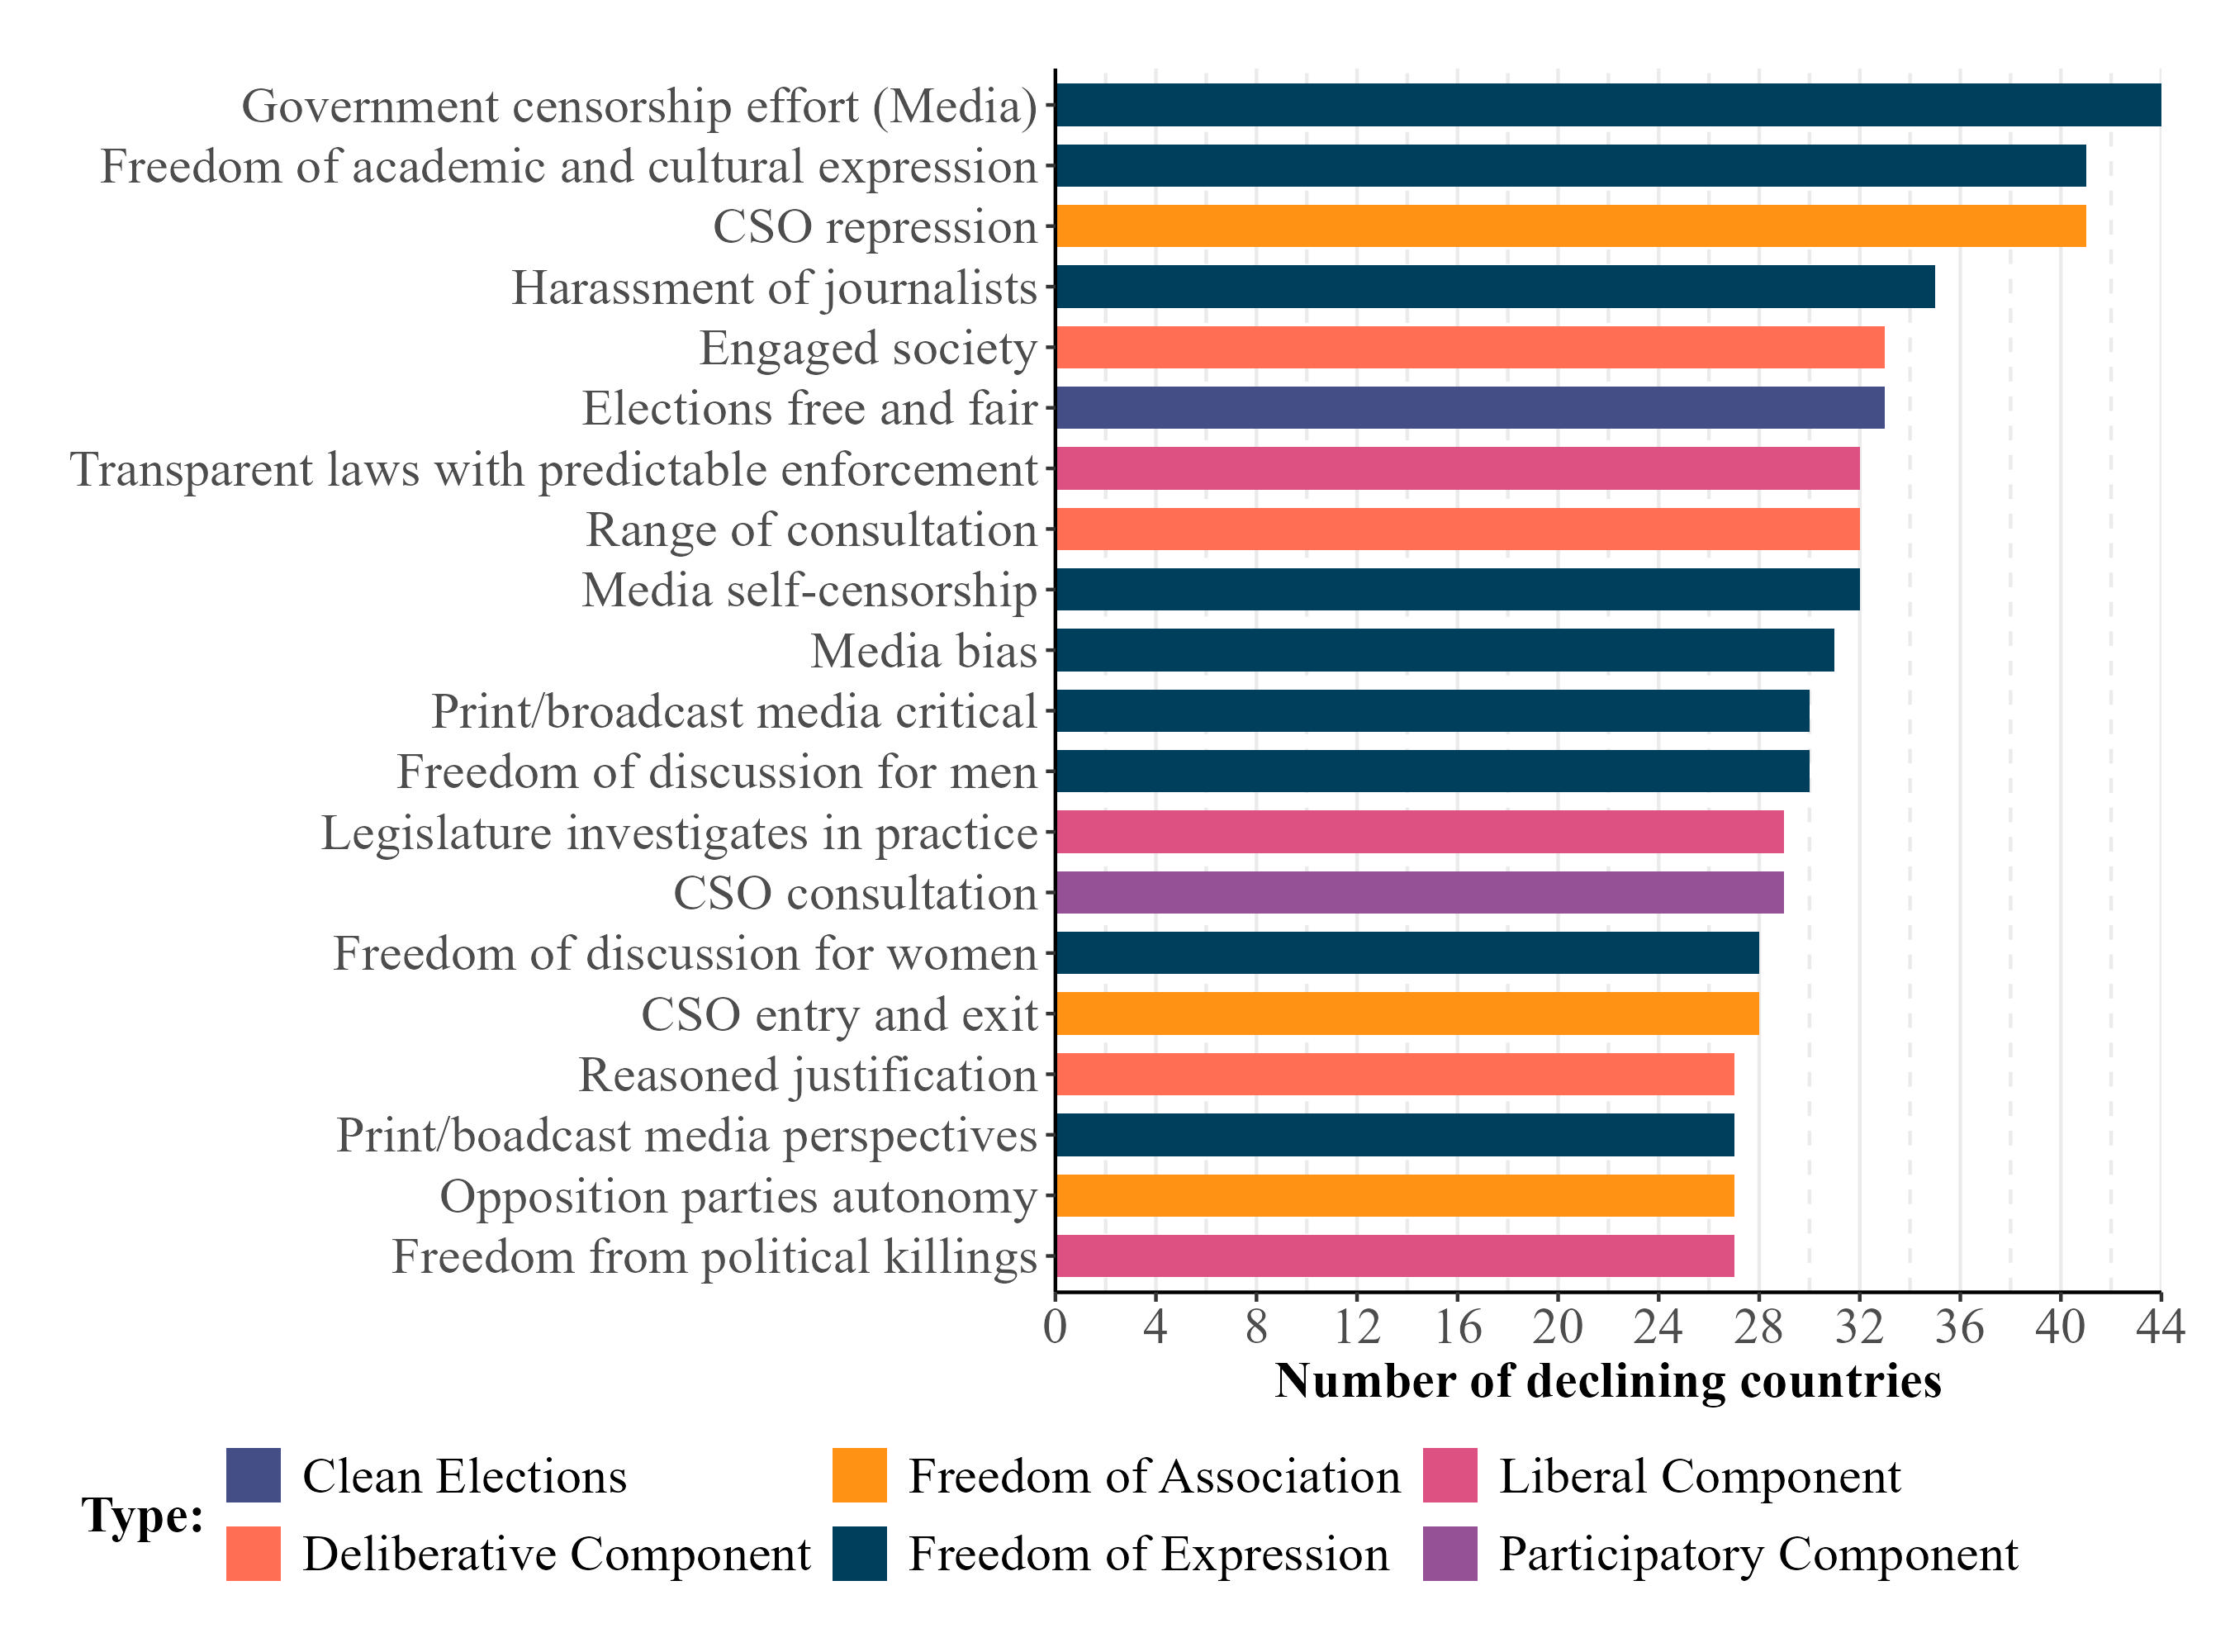
\includegraphics[width=\linewidth]{graphics/declining_indicators.jpeg}
    \caption{Top-20 declining indicators 2013-2023 \citep[p. 17]{nord_democracy_2025}}
    \label{fig:declining}
\end{figure}

Since freedom of expression, as I have accounted for above, is integral to any rigorous definition of autocracy, it is important to look at this variable in isolation, as connections between other variables and the level of democracy might be obscured by improvements in other indicators.

\section{Defining Autocracy}
Autocracy is most often identified in the negative -- the absence of fundamental components of democracy -- and our discussion of autocracy should thus start by defining democracy \citep{dahl_polyarchy_1971, przeworski_democracy_1991, schumpeter_capitalism_2010}. Of course, this is far from easy, as democracy can be hard to define, and this has led to a proliferation of subtypes of democracy. This proliferation might lead to conceptual confusion making it hard to compare research \citep{collier_democracy_1997}. For instance, one article I will focus on later in this chapter, \citet{tansey_ties_2017}, focus on the effect of linkages on autocratisation only for hybrid regimes. This might make it harder to compare directly against my own study. 

A popular way to avoid the problem of conceptual stretching is to use a minimal definition of democracy.\footnote{The problem of conceptual stretching is a considerable one when defining democracy, however, as there is no room for a lengthier discussion of this, I will restrict myself to point out some well-articulated viewpoints on the matter: \citealp[see:][]{alvarez_classifying_1996, collier_conceptual_1993, sartori_concept_1970} for a discussion of concepts, and for democracy in particular, \citealp[see:][]{collier_democracy_1997}.} This can of course be done by using the plane meaning of the word: rule by the people. This might seem a good enough definition for some; however, the statement is far too broad to be useful in a scientific context. Questions such as: how is this power executed? and how are the decisions made? naturally comes to mind.

Two famous definitions have been put forward by scholars of political science. The first one articulated was that by Joseph A. Schumpeter in his classic 1943 book \textit{Capitalism, Socialism and Democracy} \citeyearpar{schumpeter_capitalism_2010}.  Schumpeter argues that `the democratic method is that institutional arrangement for arriving at political decisions in which individuals acquire the power to decide by means of a competitive struggle for the people’s vote' \citep[p. 241]{schumpeter_capitalism_2010}. Schumpeter sees the connection between democracy and freedom of expression as important, but not a defining part of what democracy is \citep[pp. 243-244]{schumpeter_capitalism_2010}. Schumpeter's view has been adopted and explicated on by several other scholars, notable among them is Przeworski who established a list of three features necessary for a to achieve `contestation' -- the minimal point to which democracy is reducible. The three features are as follows: uncertainty of the outcome, that the outcome is irreversible, and that elections are repeated (\citeauthor{przeworski_democracy_1991} \citeyear{przeworski_democracy_1991}, pp. 10-14; \citeauthor{przeworski_modernization_1997} \citeyear{przeworski_modernization_1997}, pp. 14-18). The advantage of this approach is that it forms a concept that is highly differentiated and allows for a dichotomous definition of democracy and autocracy. 

A second, famous definition of democracy is that by Robert A. Dahl, first fleshed out in his 1971 book \textit{Polyarchy} \citeyearpar{dahl_polyarchy_1971}. Dahl's notion of polyarchy \footnote{Dahl uses the word polyarchy in stead of democracy, as he defines democracy to be an ideal type \citep[p.9]{dahl_polyarchy_1971}.} has two principal components, contestation and suffrage. Suffrage is what part of the population has the right to vote. In the early democracies this was a considerable restriction, however, in today's democracies, this right is usually given to every citizen above a certain age-threshold. Although important, it is less consequential to this study, as suffrage is very nearly universal. The second component is much more interesting for the study of contemporary democracies. Contestation is whether or not the elections are `real'. What I mean by this is: are the elections fair and consequential; is change possible? 

This type of system, polyarchy, can only come about if citizens have the opportunity to (1) formulate their preferences, (2) signify their preferences, and (3) have preferences weighted equally in conduct of government \citep[pp.2-3]{dahl_polyarchy_1971}. To achieve this, Dahl includes a list of seven institutions and five criteria for a democracy that can be seen in Figure \ref{tab:dahl} 

\begin{table}[hbt!]
\centering
\caption{\label{tab:dahl}Dahl's list of institutions and criteria}
\vspace{0.5em}
\begin{tabularx}{\textwidth} {
    >{\raggedright\arraybackslash}X
    >{\raggedright\arraybackslash}X}
\toprule
\textbf{The following institutions...} & \textbf{are necessary to satisfy the following criteria} \\
\midrule
1. Elected officials & \\
2. Free and fair elections & I. Voting equality \\
& \\
1. Elected officials & \\
3. Inclusive Suffrage & \\
4. Right to run for office & \\
\cellcolor[HTML]{003F5C}\textcolor{white}{5. Freedom of expression} & \\
6. Alternative information & \\
7. Associational autonomy & II. Effective participation \\
& \\
\cellcolor[HTML]{003F5C}\textcolor{white}{5. Freedom of expression}  \\
6. Alternative information & \\
7. Associational autonomy & III. Enlightened understanding \\
& \\
1. Elected officials & \\
2. Free and fair elections & \\
3. Inclusive Suffrage & \\
4. Right to run for office & \\
\cellcolor[HTML]{003F5C}\textcolor{white}{5. Freedom of expression}  & \\
6. Alternative information & \\
7. Associational autonomy & IV. Control of the agenda \\
& \\
3. Inclusive Suffrage & \\
4. Right to run for office & \\
\cellcolor[HTML]{003F5C}\textcolor{white}{5. Freedom of expression}  & \\
6. Alternative information & \\
7. Associational autonomy & V. Inclusion \\
\bottomrule
\multicolumn{2}{l}{\raggedright{\textit{Table copied from \citet[p. 222]{dahl_democracy_1989}, emphases are my own.}}}
\end{tabularx}
\end{table}

The requirements touch on different aspects of the process, like institutions for competition and making preferences actual policy. However, the most important take-away from this table is that, excepting voting equality, all other criteria needs freedom of expression to be satisfied.

When citizens do not have the freedom to hear or form opposing views of whatever regime is in place, contestation is imperfect. It is this aspect that Dahl's definition manages to encapsulate. Dahl's definition has another advantage, which is that it better captures the many different ways in which democracy can be hollowed out if we use a procedural minimum definition \citep{varol_stealth_2015}. Since the world is rarely possible to divide into neat and absolute categories, this better captures the complexity of real life. China and Singapore might serve as examples of this. Both regimes are authoritarian, but the average citizen have much more input on the governance of the country like Singapore than in China \citep[pp. 62-63]{nord_democracy_2025}.\footnote{Both China and Singapore are classified as autocracies in 2024 having an Electoral democracy score lower than 0.5. However,  while Singapore is an electoral autocracy \citep[p. 14]{nord_democracy_2025} with a score of 0.41, China is a thoroughly entrenched closed autocracy with a score of 0.04.\citep{nord_democracy_2025}} 

Having based my definition of democracy on Dahl's polyarchy, an autocracy can be defined as a regime that is insufficiently democratic. But at what point should the distinction be made? As we are not using a dichotomous definition of democracy, this point is of less importance. A country can be more or less autocratic to the extent that it incorporates Dahl's seven institutions. A country might have free election, but the regime controls the media. In this case it is democratic in the sense it has voting rights, but autocratic in the sense that the government controls the flow of information. If I were to give it a name I would call it an electoral democracy if the governments control of the media was fairly light, but an electoral autocracy if it was hard.\footnote{The terms electoral democracy and electoral autocracy comes from the Regimes of the World dataset included in the V-Dem data (\citeauthor{coppedge_v-dem_2025} \citeyear{coppedge_v-dem_2025}; \citeauthor{coppedge_v-dem_2024-1} \citeyear{coppedge_v-dem_2024-1}, pp. 292-294).} The fact that there is seven institutions, all of which incorporate many variables makes it a hard to define. In the real world, democracy is usually defined with these institutions in mind, and expert coders rate each country on each of the institutions. This gives a total democracy score, and this is used to separate democracies and autocracies \citep{economist_intelligence_unit_democracy_2024, marshall_polity5_2020, coppedge_v-dem_2024-1}. In the case of the V-Dem data, the Electoral Democracy Index (EDI), which approximates Dahl's polyarchy, is a measure from 0 to 1, where a regime scoring lower than 0.5 is usually put as the critical threshold for autocracy (\citeauthor{lindberg_ordinal_2016} \citeyear{lindberg_ordinal_2016}; \citeauthor{luhrmann_regimes_2018} \citeyear{luhrmann_regimes_2018} p. 64).\footnote{Note that \citet{luhrmann_regimes_2018} includes some other condition where some countries can be counted as autocracies even if their EDI score is greater than 0.5.}

We have in this section taken a closer look at the definition of democracy and autocracy and have come to the conclusion that an autocracy is the absence of certain criteria, notable among them is freedom of expression. This is the definition that will be used henceforth as we pivot to look at autocratisation. 

\section{Autocratisation}
Samuel P. Huntington's \textit{The third way} \citeyearpar{huntington_third_1991} was a game changer in the study of democratisation. Huntington conceptualised democracy occurring in waves -- periods in time where several countries turned democratic all at once. When he was writing in the late 1980's and the first years of the 1990's, he could not have known that the third wave would continue for several more years after that point. However, Huntington rightly saw in the data a second type of wave, a reversed wave of democratisation. Not only that, he also saw the beginning of the third reverse wave, or as we better know it today, the third wave of autocratisation \citep{huntington_third_1991}. 

\begin{figure}[hbt!]
\centering
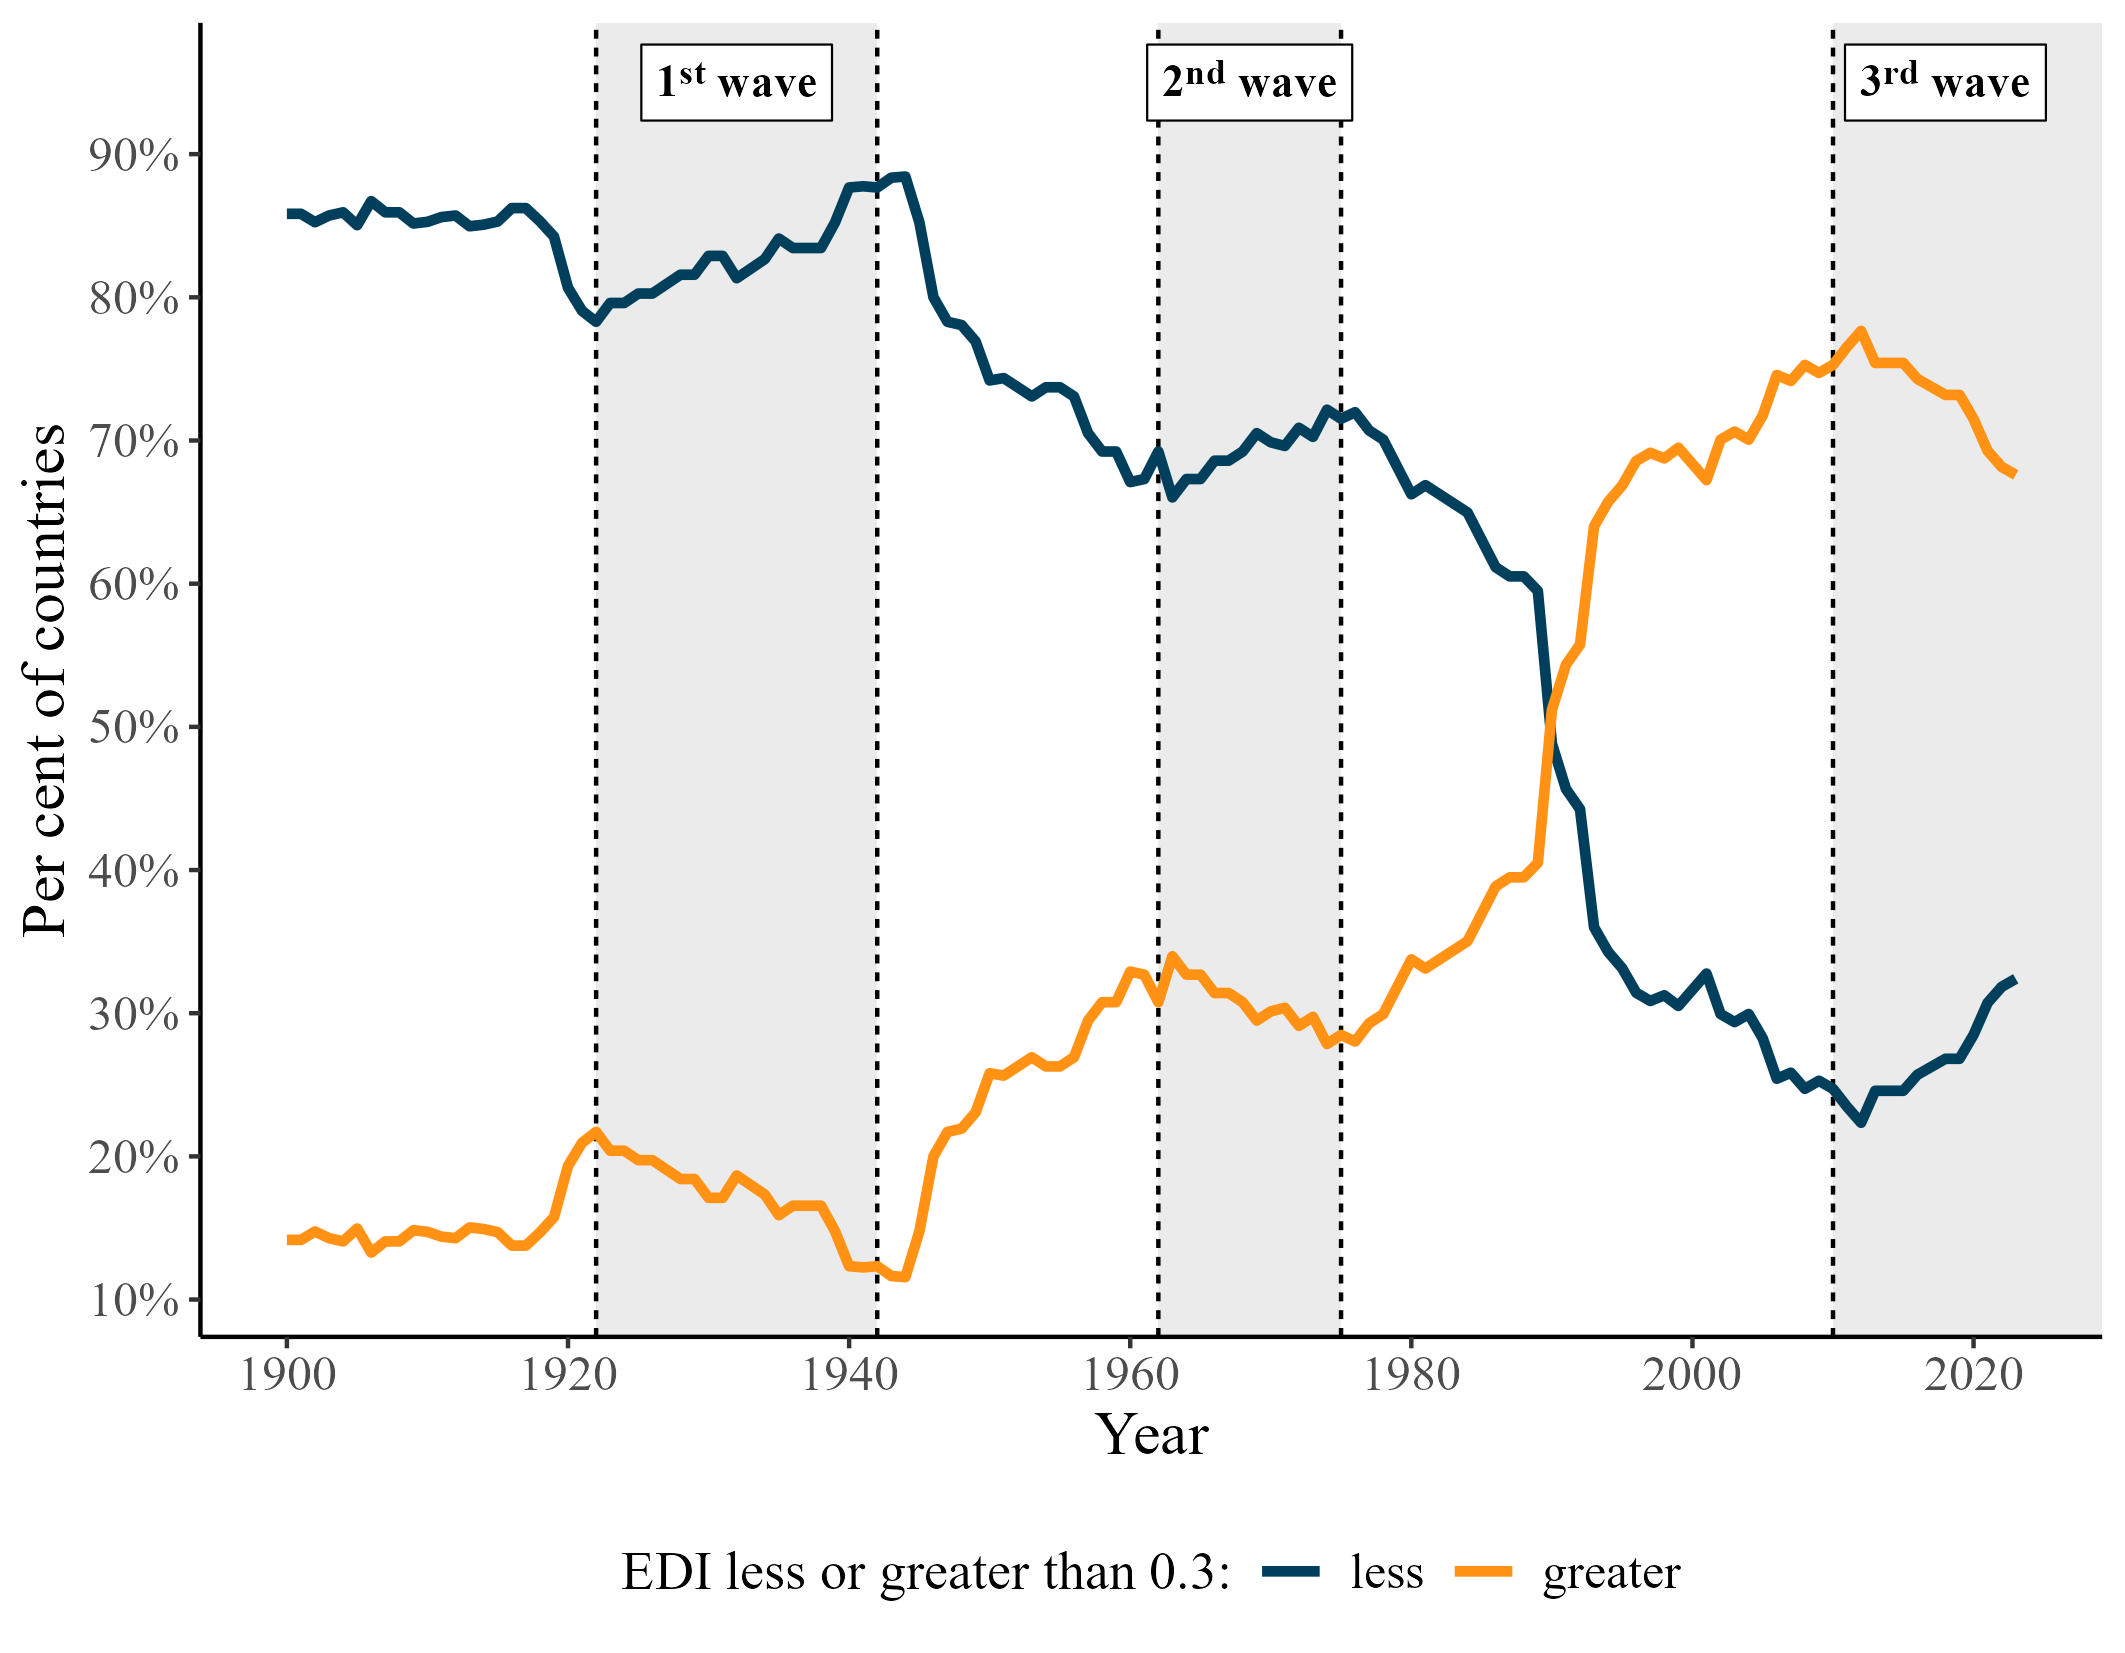
\includegraphics[width = \textwidth]{waves.jpeg}
\caption{\label{fig:autocratisation}The three waves of autocratisation}
\end{figure}

Using the Electoral Democracy Index (EDI) \citep{coppedge_v-dem_2025}, Figure \ref{fig:autocratisation} shows the proportion of countries with an EDI score greater or less than 0.3. The index is measured from zero to one; however, as the scores are very low for most countries, a threshold of 0.5 would historically be far too high to see evidence of Huntington's waves. The grey fields on Figure \ref{fig:autocratisation} show when the waves of autocratisation are taking place. The dates of the first two waves are roughly taken from \citet[p.16]{huntington_third_1991} , the date of the third wave is placed similar to the two first waves, at the point where the number of countries with an EDI score below 0.3 begins to grow. Today we are still near an all-time high, however, the recent decline in the number of democratic countries have been noticeable. 

As can be seen from Figure \ref{fig:autocratisation} authoritarian regimes are on the rise after a long period of decline. A similar figure appears in \citet{luhrmann_third_2019}, but with slightly differing dating of the waves. Scholars are now furiously debating how and why the current wave of autocratisation is happening. The process of autocratisation is being described as a slow one, legitimised by the very institutions of democracy \citep{varol_stealth_2015, bermeo_democratic_2016, luhrmann_third_2019}. This is markedly different from previous waves of autocratisation that were more dramatic \citep[pp. 6-8]{bermeo_democratic_2016}, often involving the military. What has also worried proponents of democracy is the fact that a larger part of the autocratising countries have been institutionalised democracies \citep{luhrmann_third_2019}. 

Much research has also been done on autocratisation. The reasons can be divided into two categories by the main factor: domestic or external, where the former is far more widely discussed than the latter. The domestic factor will be discussed in this section, and it is also going to touch on some ancillary external factors. The focus of this thesis is not domestic factors; however, we cannot disregard that these variables have an influence on the state of democracy in a country, some of which may possibly have an effect on the the extent to which a population enjoys the rights accorded to them in free societies. The main discussion of external factors will come in the section below.

\subsection{Domestic Factors of Autocratisation}
Economic prosperity and democracy go hand in hand. This is most famously explicated on by \citet{lipset_social_1959} in what has now become known as \textit{modernisation theory}, which sees economic development as a necessary precursor for the development of democracy. As the third wave of democratisation has created a lot of new democracies, it would not be unreasonable to think that some of the poorer countries will revert, as they do not have the resources to maintain a democratic system of government. Lipset's theory has had its fair share of critics, but even in spite of aberrations like Turkey's backsliding in the late 2010's, new studies shows evidence that the correlation between economic development and democracy is still very robust \citep{brownlee_limited_2017}.

Similar to modernisation theory, there is evidence that economic grievances, like generation differences caused by financial depressions \citep[pp. 132-174]{norris_cultural_2019}, losing out on globalisation \citep{ballard-rosa_economic_2021}, and missing out on the growth in home prices \citep{ansell_sheltering_2022}, has had an effect on the peoples commitment to democratic values. This is not universally accepted as some argue that economic factors only constitute a small part of the equation \citep{margalit_economic_2019}.

According to \citet{margalit_economic_2019} cultural factors plays an even bigger part in explaining peoples commitment to democratic values, and this has received much support. Religion \citep[pp.72-85]{huntington_third_1991}, immigration (\citeauthor{dinas_waking_2019} \citeyear{dinas_waking_2019}; \citeauthor{norris_cultural_2019} \citeyear{norris_cultural_2019}, pp. 175-212), intergenerational differences \citep{foa_youth_2020, foa_danger_2016, norris_cultural_2019, wuttke_have_2022}, majoritarianism \citep{grossman_majoritarian_2022, wunsch_demand_2023}, and party identity \citep{abramowitz_united_2019, bisgaard_how_2019, graham_democracy_2020, iyengar_strengthening_2018, krishnarajan_rationalizing_2023, peterson_partisan_2021, singer_fiddling_2023} have all been suggested to influence peoples commitment to democratic values, however, no consensus has emerged and some of the findings are contradictory (see for instance \citeauthor{schafer_cultural_2022} \citeyear{schafer_cultural_2022} for a rebuttal of \citeauthor{norris_cultural_2019} \citeyear{norris_cultural_2019}). 

The finger has also been pointed at elites and their actions. Political parties have been critiqued for lacking responsiveness to the demands of their constituents or opening the field to populist \citep{berman_causes_2021, grzymala-busse_failure_2019}. Others have indicated that elite behaviour can influence the electorate \citep{broockman_causal_2017, clayton_elite_2021}, and thereby undermine democratic norms.

Domestic factors are important for explaining autocratisation, but there is no agreement as to what extent domestic factors alone can be said to drive the current wave of autocratisation. A different approach might help us explain the phenomenon more thoroughly, which to look at exogenous factors.

\subsection{International Factors of Autocratisation}
The most obvious way for a foreign country to affect democracy in a country is by simply conquering it. If you were to look at a map showing the level of democracy in Europe for each year in the period between 1930--1945, you would see a conspicuous drop in the number of democracies. The reason is obvious, the Nazis conquered their neighbours in quick succession, thereby instituting direct Nazi rule or creating unelected puppet governments to take charge. We can see this even today, with the Russian invasion of Ukraine. Nowadays the effect is usually more subtle, where autocratisers work through the media, support preferred parties, and use diplomatic and economic coercion. However, this phenomenon is not very well understood, as many of the states acting to support authoritarian regimes are themselves authoritarian `black boxes', whose policies rarely reach the light of day.  

After the 2016 US election, where Russian interference had been considerable \citep[pp. 14-15]{mueller_report_2019}. The effect is at present indeterminate, \citet{zhuravskaya_political_2020} notes that there is a reasonable possibility that social media might have an effect, however, as \citet{eady_exposure_2023} and \citet{guess_reshares_2023} state: the Russian social media campaigns does not seem to be reaching all that far. 

The last external factor I look into, is theories about how the existence of other authoritarian regimes might increase the number of autocratising regimes. This is known as autocratic diffusion and will be the topic of the next section, as it will be a foundational element of the thesis.

It is apparent that there are multitudes of explanations available as to why countries autocratise \citep{berman_causes_2021}. None are well enough understood, however, they have received more or less treatment in the current literature. The better studied explanations are the internal ones. From early on it was established that there was a strong correlation between socio-economic factors and democracy. This has led to a wealth of studies on this area. The external factors are less well studied, and with better and faster channels of communication this has likely become a more influential factor in autocratisation.

\section{Autocratic diffusion}
As has been shown in the previous section, reasons for the current wave of autocratisation are numerous and the strength of each explanation is a matter of widespread debate. This section will narrow this down to a focus on external factors, specifically that of autocratic diffusion. Ideas, values, and learning matter in international politics \citep[pp. 86-92]{mingst_essentials_2019} as they are crucial to the integrity of every national polity.

Diffusion was already pointed out as a reason for the wave-like nature of democratisation by \citet{huntington_third_1991}. It did not get a thorough discussion, probably because at the time it seemed rather small and inconsequential. Huntington referred to it as `snowballing,' because the process is analogous to a snowball getting bigger and bigger as it rolls down a hill. The more autocratic countries there are, the greater the likelihood is that other countries also become autocratic.

By diffusion is meant `any process where prior adoption of a trait or practice in a population alters the probability of adoption for remaining non-adopters' \citep[p. 325]{strang_adding_1991}. And it has been used to understand organisations \citep{dimaggio_iron_1983}, decolonisation \citep{strang_adding_1991}, and democracy \citep{elkins_waves_2005}. \citet{elkins_waves_2005} places diffusion as one of three major reasons for the cluster-like behaviour in the international system. First, a pattern of similar decisions can be taken by countries as individual responses to similar problems. Second, a pattern may emerge because the responses to problems are coordinated by organisations or hegemonic powers. This can occur by way of cooperation, horizontal, or by coercion, vertical. The third is diffusion, where decisions are interdependent but uncoordinated. 

The framework was in large part developed to study organisations and democratisation \citep{elkins_waves_2005, huntington_third_1991}. However, around 2010, it had become apparent that a new wave of autocratisation was occurring, and diffusion has become a popular way of explaining it \citep{ambrosio_constructing_2010, gelman_authoritarian_2008, lankina_authoritarian_2016, weyland_autocratic_2017}. One reason why it may have become in vogue to explain autocratisation in terms of exogenous explanations is that several rich and institutionalised democracies have begun autocratising. This might in turn have led to a de-emphasis modernisation theory and a search for new explanations. Adding to this, the existence of several large, prosperous, and stable autocracies is a highly probable reason of the shift in how researchers try to explain the waxing and waning of democracy in today's world. 

\section{Factors in Autocratic Diffusion}
We turn now to some factors that previous research has pointed at being likely, or unlikely, to affect how ideas spread. The first two sections consider what reason might be best able to explain why regimes have an effect on the level of democracy in a country; is it the exporters of authoritarianism, countries like China or Russia, that intentionally try to autocratise other countries or is it the regimes in the influenced countries themselves who look for a patron in the influencers. This is a question of supply or demand, where the first explanation put weight on autocratic `black knights' for supplying -- or spreading -- authoritarianism. The second explanation puts weight on demand-side explanations, reasoning that as a consequence of authoritarian states becoming more important in the international system, authoritarian leaders in weaker countries can seek to use their support as a shield or as an example to learn from. 

The third section considers the mechanisms through which this influence is exerted, namely linkages. The theory is that every type of linkage, whether diplomatic, economic, security related, or social, may facilitate the spread of authoritarian ideas and solutions. I will show how the concept of linkages was developed, and how it came to be used in the study of autocratisation. 

\subsection{Authoritarian influencers}
To some observers, the reason why diffusion works is that dominant autocracies in the international system is intentionally trying to either cajole or force countries to become autocratic. This theory begs the question: why would autocrats prefer their neighbours to be autocratic? Some have proposed that it is purely driven by interests, other by the ideology of the exporting countries \citep{weyland_autocratic_2017}.  \citet{weyland_fascisms_2017} studies the fascist regimes in Italy and Germany, \citet{de_la_torre_hugo_2017} examines the leftist regimes in Venezuela and Bolivia, \citet{darwich_creating_2017} looks at the Muslim Brotherhood, and \citet{buzogany_illiberal_2017} traces the development of `illiberal' democracy in Hungary. 

The fascist regimes in Europe, and the leftist regimes in Latin-America were all `missionary' regimes, that is to say, they try to spread their ideology and system of government. However, most modern regimes are more concerned with their immediate interest rather than spreading their authoritarian model \citep{bank_study_2017, brownlee_limited_2017}. 

According to the above studies, the autocratic influencers of today are spreading authoritarianism because it is in their own interest, however, is the spread of authoritarianism an intentional strategy of influencers? There is nothing obvious that indicates this should be the case, other than maybe a fear of democracy `infecting' the autocratic influencer itself. Recent research has examined this hypothesis in greater detail by shining the spot-light on several large autocratic countries, such as: China \citep{chen_democracy_2015, hackenesch_not_2015}, Russia \citep{babayan_return_2015, delcour_spoiler_2015}, and Saudi Arabia \citep{freyburg_local_2015, hassan_undermining_2015}.  They all find that in most cases `autocratisers' are not intentionally spreading their system of government. They are usually only protecting their interest, and as a consequence autocratisation happens \citep{risse_democracy_2015, borzel_noble_2015}. This indicates that the impetus is not on the part of the influencers, but rather on the influenced. 

It seems obvious, then, that in most cases, major autocratic countries are not trying to spread their ideology, but that does not mean that they do not affect other countries. When leaders look for for ways to strengthen their grip on power, the existence of other successful authoritarian states may influence their decisions. This might happen through learning or normalisation of conduct. Considering that autocratisation is most likely to be demand-driven, I now turn to a discussion of the mechanics of demand-driven autocratisation.

\subsection{Authoritarian demand}
The last section made clear an interesting point, the main thrust for autocratisation is not likely to be emanating from the authoritarian `black knights,' like China and Russia. They seem more preoccupied with keeping the status quo, looking for stable partners, rather than type of regime. This is also the case for democracies, where there are indications that they prefer stability over democracy \citep{hassan_undermining_2015, risse_democracy_2015}.

What have received less attention is the confluence of domestic and international factors, where autocratisation is only supported by international connections. \footnote{\citet{buzogany_illiberal_2017} discusses this to some extent, where autocratisation happens both in conjunction with diffusion and because of strictly domestic ones.} International factors may in this scenario serve as a necessary condition for autocratisation, but they are unlikely to be sufficient. Hypothetically, regime leaders would likely have more freedom? to manipulate certain fundamental components of democracy if they are not alone and have some tacit support from their peers. 

There are several ways to study this phenomenon. A deep dive into cases is one possibility, another is to examine disaggregated components; whereby they might serve to give us a better understanding of how diffusion works and build a logical structure of the paths and mechanisms of how the international component might influence autocratisation. The work has already been started, but except for a couple of recent studies \citep{gamso_is_2021, toettoe_foreign_2023}, focused on the media, this is virgin territory. 

In Table \ref{tab:mechanism} below, I summarise the main reasons that are proposed for why we can see traces of authoritarian diffusion and what the literature has so far concluded on each of them. I also specify what will, and will not, be a part of my thesis.

\begin{table}[!hbt]
\centering
\caption{\label{tab:mechanism}Toettoe and Jiang's three mechanisms autocratic diffusion}
\vspace{0.5em}
\begin{tabularx}{1\textwidth} {
 >{\noindent\justifying\arraybackslash\hsize=.13\hsize}X 
 >{\noindent\justifying\arraybackslash\hsize.2833\hsize}X 
 >{\noindent\justifying\arraybackslash\hsize=.2833\hsize}X 
 >{\noindent\justifying\arraybackslash\hsize.2833\hsize}X}
\toprule
& \textbf{Influencer} 
& \textbf{Demand}
& \textbf{Norm} \\
\midrule
\textit{Mechanism}
& China seeks to export its model and extend ties to autocratic countries 
& Autocratic leaders seek to consolidate their regime and extend ties to China 
& Passive spread of undemocratic norms \\
\addlinespace
\textit{Actions} 
& Material support for autocratic regimes, sharing techniques and laws aimed at suppressing dissent, and providing an alternative to liberal norms 
& No formal conditions related to democracy promotion, gain access to capital markets and political arenas, and learn how to regulate media and crack down on dissent 
& Because of exposure to China, actors inside the countries internalise autocratic norms and values \\
\addlinespace
\textit{Literature }
& Unlikely, as there is little evidence that today's authoritarian countries try to export their model. They might still be willing to share their knowledge, but this is not the main purpose of extending assistance.
& Likely, as the world has become less democratically unipolar and regimes are likely to be needing willing allies to not be shunned by the rest of the world when autocratising.
& Likely, as examples of successful autocracies, like China, proliferates, and democratisation is no longer considered the only way to become successful.\\
\addlinespace
\textit{Implications}
& Will not be a focus of the study, because it is unlikely.
& Is the main focus of the study.
& Will not be a focus of the study, because it is outside the limits of the study. \\
\bottomrule

 \multicolumn{4}{p{\textwidth}}{\raggedright{\textit{Mechanisms are found in \citet[pp. 29-31]{toettoe_foreign_2023}}}}

\end{tabularx}
\end{table}

\section{Linkages}
A possible way in which to examine authoritarian diffusion is through \textit{linkages}. Diffusion spreads by contact, and more linkages to authoritarian countries, especially influential ones, is one of the best ways of studying the phenomenon. 

The importance of linkages in studying international factors in regime change was first espoused by \citet{levitsky_linkage_2006}. In their study, they divided the international dimension into leverage and linkage, where the former is `the degree to which governments are vulnerable to external democratizing pressure' and the latter is defined as `the density of ties (economic, political, diplomatic, social, and organizational) and cross-border flows (of trade and investment, people, and communication)' \citep[p. 379]{levitsky_linkage_2006}. They found that Linkage was better at explaining democratic outcomes than was leverage, and that when they appeared together they were an even better explanation \citep[pp. 388]{levitsky_linkage_2006}.

While \citeauthor{levitsky_linkage_2006} originally used the concept of leverage and linkages to study democratisation, other authors have used the concept to great benefit in the study of autocratisation. This has happened both on an aggregated level where researchers look at the world as a whole \citep{ambrosio_constructing_2010, hall_authoritarian_2017, tansey_ties_2017}, and on the level of case studies on countries like: Cambodia \citep{loughlin_chinese_2021}, Myanmar and Thailand \citep{wong_chinese_2019}, and Turkey \citep{yilmaz_authoritarian_2020}. 

Linkages offer one of the most plausible tools for investigating external factors of regime change and/or regime stability. \citet[pp. 383-386]{levitsky_linkage_2006} proposed four main ways in which linkages could be a source of anti-authoritarian pressure. The first is that linkages heighten the international salience of autocratic abuse, the second is that it increases the likelihood that western governments will take action in response to abuse, the third is that linkages shift domestic preferences in a pro-democratic direction, and finally the fourth is the reshaping of the domestic balance of power within authoritarian regimes. These are still some of the primary mechanisms proposed for explaining one of the most important external factors of democratisation. Notwithstanding the importance of the contribution, the actual mechanisms they proposed is actually not that helpful when trying to explain autocratisation, as there are likely different pressures working on the countries. 

\begin{table}[p]
\centering
\caption{\label{tab:linkage}Four principal mechanisms of linkage effectiveness}
\vspace{0.5em}
\resizebox{\textwidth}{!}{
\begin{tabularx}{\textwidth} {
 >{\centering\arraybackslash\hsize=.20\hsize}X 
 >{\noindent\justifying\arraybackslash\hsize=.40\hsize}X 
 >{\noindent\justifying\arraybackslash\hsize=.40\hsize}X}
\toprule
& \textbf{\citeauthor{levitsky_linkage_2006}} & \textbf{\citeauthor{tansey_ties_2017}} \\
\midrule
1\textsuperscript{st} mechanism 
& \textbf{Increased salience of autocratic abuse}
& \textbf{Decreased salience of autocratic abuse}  \\
\addlinespace
 & Autocratic abuses in high-linkage countries gain attention in the West and internationally, while this does not happen to the same degree in low-linkage countries. 
 & Autocratic patrons do not value democracy, and countries with a higher number of autocratic linkages are less likely to face sanction and international isolation if they stay autocratic. \\
\addlinespace
2\textsuperscript{nd} mechanism 
& \textbf{External stakeholders}
& \textbf{External stakeholders} \\
\addlinespace
 & With greater attention put on it and by the existence of prodemocratic stakeholders in the affairs of the regime, there is a greater likelihood that western governments will take action in high-linkage countries. 
 & Autocratic patrons can sponsor other autocratic regimes, serving to uphold them. There is also the fear of a democratic contagion spreading through the linkages, and this might increase the likelihood that autocratic partners will co-operate. \\
\addlinespace
3\textsuperscript{rd} mechanism
& \textbf{Domestic stakeholders}
& \textbf{Domestic stakeholders} \\
\addlinespace
 & Linkages to the global West creates domestic stakeholders, especially business leaders and western-educated elites, who have something to lose from international isolation. And this might give an impetus to pushing the country further in a prodemocratic direction to gain benefits from the West.
 &  Where the number of autocratic linkages is high, domestic stakeholders are incentivised to maintaining the status quo and avoid regime change. I.e., not push for democracy. \\
\addlinespace
4\textsuperscript{th} mechanism
 & \textbf{Balance of power}
 & \textbf{Learning} \\
\addlinespace
 & Linkages to democratic countries can protect vulnerable opposition groups by putting them in the spotlight, which makes repression more difficult, or financial support might keep them fighting for democracy. Finally, linkages might strengthen reformist tendencies in autocratic parties because of frustration with international isolation
 & The fear of democratic contagion between countries might serve to facilitate learning and emulation. This can be through sharing technologies and policies aimed to restrict political and civil liberties, which are conducive to democracy and might weaken autocratic regimes. \\
\bottomrule
 
 \multicolumn{3}{p{\textwidth}}{\raggedright{\textit{Mechanisms are found in \citet[pp. 383-386]{levitsky_linkage_2006} and \citet[pp. 1225-1227]{tansey_ties_2017}}}}

\end{tabularx}
} % End resizebox
\end{table}

Taking up the discussion from \citeauthor{levitsky_linkage_2006}, \citet{tansey_ties_2017} repurpose the theory of linkages for their study on autocratic regime survival. In this paper, the authors tease out `four principal causal mechanisms that link autocratic linkage to autocratic survival' \citep[p. 1225]{tansey_ties_2017}. These resemble and mirror the mechanisms of \citeauthor{levitsky_linkage_2006} on a surface level, but they work in different ways. The mechanisms are as follows: Firstly, linkages create domestic stakeholders to maintain the status quo; second, it decreases the likelihood that autocratic, or autocratising, countries are targeted for sanctions; third, linkages increase the stakes that external actors have in the domestic regimes of other countries; and finally, they can facilitate processes of learning and emulation \citep[pp. 1225-1227]{tansey_ties_2017}. To highlight the similarities and clarify the mechanisms, table \ref{tab:linkage} shows the theories side by side. 

It should not come as a surprise that the \citeauthor{tansey_ties_2017} study is more suited to my purpose of creating a theory of how links to autocratic patrons affect the level of freedom of expression. At the same time, it is important to trace its origins and background, as it is to no small degree a reworking of \citeauthor{levitsky_linkage_2006} to fit a research agenda that focus on the opposite phenomenon. 

In \citet{tansey_ties_2017}, and to a smaller degree \citet{levitsky_linkage_2006} we have the start of a theory. They can guide us on some distance on the way, but the theories are not yet suited fully to our purpose. I am going to face this challenge in the next chapter, where I build a theoretical framework on the back of these two vital contributions. What I would like to emphasise from this section is the indispensable nature of these two works in the study of democratisation and autocratisation. 

\section{The Gap in the Literature}
As can be seen from the amount of recent contributions to the study of both linkages and diffusion, this is a growing field. But as of yet, there are no clear answers. One particular avenue that is understudied is how linkages to autocracies actually work to undermine democracy. There have recently been published a couple of studies on how linkages to China affects the media \citep{gamso_is_2021, toettoe_foreign_2023}, however these are in the minority.

Most of the contributions are only focused on how the linkages affect democracy \citep{bader_china_2015, levitsky_linkage_2006, risse_democracy_2015, tansey_ties_2017, weyland_autocratic_2017}. And the first studies focused exclusively on regime survival \citep{bader_china_2015, tansey_ties_2017}. But with the recent evidence from \citep{gamso_is_2021, toettoe_foreign_2023} there is a possibility that autocratic countries might have an autocratising effect, not just increasing the survival rates of already autocratic regimes. However, this effect might not be discernable at the level of democracy. 

With this study I want to know more about how linkages affect democracy by examining a single component of democracy, namely freedom of expression. This is an understudied part of the literature on democratic backsliding. In addition, if I find that linkages to China have an impact on freedom of expression, it would help us to understand the current autocratisation much better. There are some preliminary evidence that this is possible from \citet{gamso_is_2021} and \citet{toettoe_foreign_2023}, which both concern the repression of the media. Based on this evidence it is plausible that linkages to China affect freedom of expression. Freedom of expression is also, as we have seen, the fastest declining component of democracy, making it particularly interesting area of enquiry. 

\section{Summary}
In this chapter I have discussed previous scholarship on freedom of expression and how this links up with the study of autocratic diffusion. This is a complicated topic; however, I have discussed how freedom of expression fits into the larger context of studies on democratisation and autocratisation. I have also looked at several of the research avenues that are currently being pursued, leading us to focus our attention to linkages between countries. 

In the rest of this thesis, I extend this line of research focusing on freedom of expression, as it is an integral component of democracy. I do this by using the linkages countries have to China, one of the most influential and likely ways in which foreign countries can have an impact on freedom of expression in other countries.

\chapter{Theory} \label{chp:theory}
\lettrine{C}{entral to this study} is the mechanism by which China may influence the countries it has linkages with. Diffusion theory teaches us that there are many ways in which the international component can affect the level of, first and foremost, democracy, but also the level of freedom of expression a populace enjoys. To truly understand how our independent variable links to our dependent variable, a more detailed treatment of this relationship is necessary.

To remind the reader, the research question asks whether a country's linkages to China affect the extent of freedom of expression in that country. It is not immediately obvious that they should, but in this chapter, I propose first that they do, and second that the effect of linkages will be moderated by regime type. The following sections explain this in greater detail, but I posit that linkages to China may have a negative impact on freedom of expression in other countries because of a confluence of different factors. I there to be three main reason as to why linkages can impact internal affairs in a country. These are learning, immunity, and displacement. Where learning refers to linkages enabling countries to learn from China. Immunity refers to being supported by China when autocratisation. And lastly, displacement refers to how China is displacing Western democratic countries as a favoured partner, and thus weakening the democratic influence capacity Western countries have on their partner countries.

\section{The Framework}
In this section I build the framework for studying how dyadic linkages might influence freedom of expression. This framework is built up around the three mechanisms mentioned briefly above, and will be expended on in due time. Here I show the rough outline of my theory, before further elaborating on each mechanism in the next three sections. 

I have noted the importance of the contribution of \citet{tansey_ties_2017}, however, it is not a perfect fit. The first problem is that the study concerns authoritarian regime survival and not, as is the case here, with the possibility that an increase in linkages may subsequently increase the authoritarian characteristics of a regime. The second problem is that the \citeauthor{tansey_ties_2017} study is explicitly concerned with ruling out the effect of influential autocratic regimes---so called `black knights' \citep[p.1232]{tansey_ties_2017}. This is the opposite of what this thesis is trying to do. As this is a substantial difference, I will have to make some alterations to the causal mechanisms as proposed in \citet{tansey_ties_2017}. 

The mechanisms of learning and what I have chosen to refer to as immunity---a concept very close to what is termed `decreased salience of autocratic abuse' in Table \ref{tab:linkage}---is going to continue to play a big part in my own theoretical framework. In contrast, the mechanism connected to external stakeholders, in my case China, will stay more in the background. The reason for this is that some contributions find only limited support for this mechanism in regards to China \citep{chen_democracy_2015}. Displacement is a term I use for a phenomenon where linkages to China displaces those of Western countries. The gist of it is that as China becomes more prominent in the international order, it will start to take more space. This space was previously occupied by Western countries, but as time passes, China is taking their place in many different spheres, be they economic, political, or security related. I deem it likely that Western democratic countries engage in some form democracy support \citep{levitsky_linkage_2006}.\footnote{Accepting that this is not always what happens \citep{chen_democracy_2015, wong_chinese_2019}} 

My theory can be summed up by Figure \ref{fig:theory}. First, I take for granted that most countries wish to establish closer linkages to China. In some cases, this might happen because some regimes tries to create a good rapport with an autocratic patron, or, and what is more likely, it happens because it is all but an economic necessity to establish closer linkages to China. This is reflected in Figure \ref{fig:link-china}, that shows how linkages to China has developed in the years between 1994 and 2023. The two dashed boxes in the upper part of Figure \ref{fig:theory} shows the assumption I make that the search for a patron and necessity are the two main reasons why countries would wish to establish linkages at all. However, an in-depth enquiry into the reason for the establishment of linkages is beyond the scope of this study. It should suffice it to say that China is today by far the most powerful autocracy in the world, and its economic power is second only to the USA. 

\begin{figure}
    \centering
    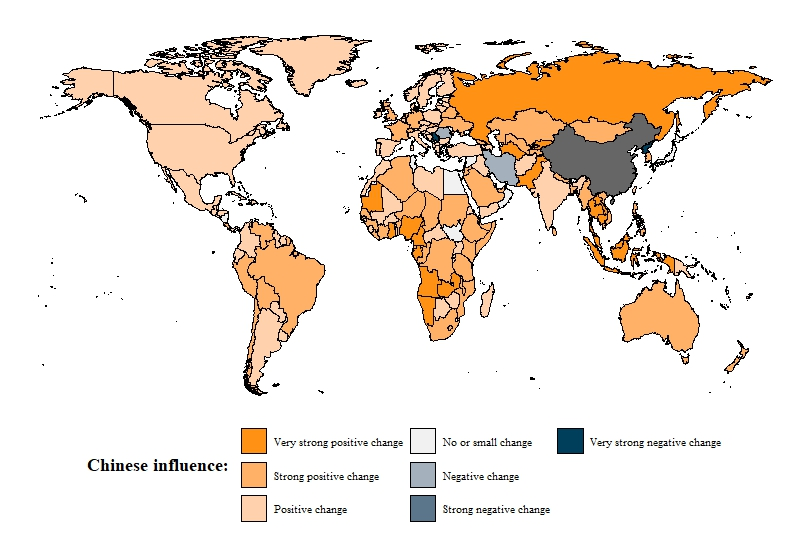
\includegraphics[width=\linewidth]{graphics/chinese_influence.jpeg}
    \caption{Development of linkages to China 1994-2023}
    \label{fig:link-china}
\end{figure}

When linkages are established, the influence of China can start to have an effect. Whether it is a supply or demand relationship is unclear. Authors have attributed it to both \citep[e.g., see:][]{ambrosio_rise_2012, bader_china_2015, brand_authoritarian_2015, economy_exporting_2020, gamso_is_2021, loughlin_chinese_2021, risse_democracy_2015, toettoe_foreign_2023, weyland_autocratic_2017}; however, the literature indicates the latter to be more plausible, with the caveat that China is using the opportunity for what it is worth. I therefore consider linkages, if they have an effect at all, to be a demand-driven mechanism, see Table \ref{tab:mechanism} for more information. 

The next level of Figure \ref{fig:theory} are the three mechanisms: learning, immunity, and displacement, that I have mentioned above. The next sections explains these three mechanisms in greater detail. These mechanisms indicates the most plausible ways in which the linkages to China may cause restrictions on peoples rigth to freely  expression their opinions. 

\begin{figure}[!hbt]
\centering
\resizebox{.8\textwidth}{!}{%
\begin{circuitikz}
\tikzstyle{every node}=[font=\LARGE]
\draw [ rounded corners = 16.2] (5,16) rectangle  node {\LARGE Linkages to China} (12.5,13.5);
\draw [ rounded corners = 16.2] (6.25,12.25) rectangle  node {\LARGE Immunity} (11.25,9.75);
\draw [ rounded corners = 16.2] (0,12.25) rectangle  node {\LARGE Learning} (5,9.75);
\draw [ rounded corners = 16.2] (12.5,12.25) rectangle  node {\LARGE Displacement} (17.5,9.75);
\draw [ rounded corners = 16.2] (3.75,8.5) rectangle  node {\LARGE Decline in freedom of expression} (13.75,6);
\draw [->, >=Stealth] (8.75,13.5) -- (8.75,12.25);
\draw [short] (5,14.75) -- (2.5,14.75);
\draw [->, >=Stealth] (2.5,14.75) -- (2.5,12.25);
\draw [->, >=Stealth] (8.75,9.75) -- (8.75,8.5);
\draw [short] (2.5,9.75) -- (2.5,7.25);
\draw [->, >=Stealth] (2.5,7.25) -- (3.75,7.25);
\draw [->, >=Stealth] (15,14.75) -- (15,12.25);
\draw [ rounded corners = 16.2, dashed] (0,19.75) rectangle  node {\LARGE Patron-seeking}  (7.5,17.25);
\draw [ rounded corners = 16.2, dashed] (10,19.75) rectangle  node {\LARGE Economic necessity}  (17.5,17.25);
\draw [->, >=Stealth, dashed] (6.25,17.25) -- (6.25,16);
\draw [->, >=Stealth, dashed] (11.25,17.25) -- (11.25,16);

\draw [short] (12.5,14.75) -- (15,14.75);
\draw [short] (15,9.75) -- (15,7.25);
\draw [->, >=Stealth] (15,7.25) -- (13.75,7.25);
\end{circuitikz}
}%
\caption{Theory of Chinese influence}
\label{fig:theory}
\end{figure}


\section{Learning}
Learning is in several contributions theorised to be one of the main vehicles of policy diffusion \citep{gilardi_four_2016, shipan_mechanisms_2008, simmons_introduction_2006}; this is not surprising as actors want to strengthen their position by using whatever methods seems to them most effective. And to do this, they look to their peers for guidance. I focus here on learning, as I see decision makers as generally being rational in adopting policies which are either for personal gain or as an end in themselves, i.e., to strengthen their country \citep{shipan_mechanisms_2008}, and believe that it is one of the main vehicles for linkages to China to have an impact on freedom of expression.

What I have simplified in this thesis as the category of `learning', is in the literature quite often divided into two separate mechanisms: learning and imitation/emulation \citep{ elkins_waves_2005, gilardi_four_2016, shipan_mechanisms_2008}. There might not seem to be much difference between them, and I would argue that in most cases there is not; however, in some cases they might be usefully separated. Learning, when used as a separate category can be defined as adopting policies after studying their effects in other places and deeming them the best option. Imitation on the other hand is defined as the adoption of policies based on their earlier adoption by peers and the appropriateness of the policy to the polity \citep[pp. 799-801]{simmons_introduction_2006}. There is much more that can be said about this difference; but, except in noting the use, it will not be relevant to distinguish between these mechanisms, and they have therefore been collapsed into a single category: learning. 

\subsection{Learning and China}

Diplomatic linkages are probably the main way learning can have an effect on the diffusion of policy. \citet[p. 385]{levitsky_linkage_2006} argues that `[l]inkages generates "soft power," or the ability to "shape preferences" and "get others to do what you want." Here diplomatic linkages are one way of achieving this, especially for dominant countries like China and Russia, which smaller countries would look to learn from.

Diplomatic or political linkages show how interconnected two polities are and can include measures like the establishment of embassies and consulates, visits by high-level officials, and participation in international organisations. With repeated interactions in these forums, countries may influence each others as they learn about the policies that the partners have enacted. 

This effect can occur through socialisation, conditionality, and the process of binding \citep[pp. 1323-1326]{ambrosio_catching_2008}. Socialisation refers to transmission of norms and values, which is likely to happen through repeated interactions facilitated by the ties. Conditionality is a more direct way of influence, when one party makes normative demands of a target state. Usually this is done by the major party. The process of binding refers to how ties might bind elites to a certain way of doing things.

When it comes to freedom of expression, these diplomatic ties might even have a more direct effect where, e.g., political ties can serve as a facilitator for teaching how to undermine freedom of expression. China is one of the most advanced countries when it comes to quashing dissenting voices. It has the know-how that other authoritarian leaders would like to get their hands on, and it shares this with other authoritarian regimes \citep[pp. 3-6]{economy_exporting_2020}. For instance, in April 2017, China held a cybersecurity training seminar for Vietnamese officials which was then followed by the introduction of a new Vietnamese cybersecurity law the next year, remarkably similar to the China's own \citep[p. 8]{shahbaz_rise_2018}. 

Some of the learning undoubtedly occurs because countries adopt what from the outside seems like sensible or effective policies from China. However, China is itself a willing teacher (\citeauthor{brazys_chinas_2020} \citeyear{brazys_chinas_2020}, p. 67; \citeauthor{repucci_authoritarians_2022} \citeyear{repucci_authoritarians_2022}, p. 50) and much of it happens through diplomatic linkages. These linkages can take the form of membership of international organisations (\citeauthor{ambrosio_catching_2008} \citeyear{ambrosio_catching_2008}; \citeauthor{economy_exporting_2020} \citeyear{economy_exporting_2020}, pp. 6-7), training of journalists (\citeauthor{brazys_chinas_2020} \citeyear{brazys_chinas_2020}, p. 50; \citeauthor{cook_countering_2022} \citeyear{cook_countering_2022}, pp. 118-119), and the establishment of think tanks \citep[pp. 15-16]{loughlin_chinese_2021} and cultural organisations like the Confucius Institutes \citep{popovic_charm_2020}. 

While the main learning happens in diplomatic forums, it can also happen with economic and security ties; however, I consider these to be strictly secondary. Stronger economic bonds to a partner might serve to socialise countries to the same behaviour; emulating what might seem to be good ideas. With security ties the same socialisation might occur, or the learning might be more direct as when a regime is taught tactics on how to repress freedom of speech. 

Assuming that Beijing is a gravity point in a security network, the closer the co-operation in the security realm, the more a country should learn from China. This learning might then appear as effective repression of freedom of expression. Security forces in countries tied to China might be taught by Chinese instructors and thereby get socialised into a normative environment where repression of freedom of speech is unproblematic. China may also give security forces effective tools for repression. Here it is very likely that they give assistance on technical infrastructure like monitoring and censoring the internet. (READ Hoffman) While both economic and security linkages are likely to have an impact, they would, most likely be moderated through a diplomatic forum, or be so known as not being part of the linkages, but rather norms; a separate issue from what we are concerned with here.

In summary, learning is likely to be a cause of policy diffusion, and, in the case that China has any influence, is a likely route in which linkages may lead to restrictions on freedom of expression.

\section{Immunity}
Immunity is another important reason why countries might limit freedom of expression when they establish linkages with China. My conception of immunity best corresponds to the mechanism that in Figure \ref{tab:linkage} is labelled `decreased salience of autocratic abuse.' However, it also includes attributes from mechanisms two and three, which are labelled external and domestic stakeholders respectively. 

The concept of immunity refers to the fact that countries, regardless of regime, must in some ways work with one another. Now, if a country upsets its major partners, this will undoubtedly have consequences. Immunity, then, is when countries can shirk on certain obligations demanded by some partners, because they have other partners who can substitute for the losses incurred. For a long time western countries were the major partners to almost every country, and this often---but not always \citep{borzel_noble_2015, wong_chinese_2019}---came with strings attached. Western countries usually promote democracy as a part of their support, and this is likely to include demands that countries refrain from repressing freedom of expression. To many leaders of autocratic regimes, this might be a problem, as to secure their power they need to rely on tactics which are diametrically opposed to freedom of expression.

\subsection{Immunity and China}

China is the opposite. China promises a hands-off approach to foreign policy. This is even enshrined in article 4 of the law of foreign relations, stating that:
\begin{displayquote}
\textbf{Article 4} The People's Republic of China pursues an independent foreign policy of peace, and observes the five principles of \textit{mutual respect for sovereignty} and territorial integrity, mutual non-aggression, \textit{mutual non-interference in internal affairs}, equality and mutual benefit, and peaceful coexistence. \citep[emphases are my own]{xinhua_law_2023}
\end{displayquote}
The two key-points here is the mutual respect for sovereignty and mutual non-interference in internal affairs. What this essential means is that China promises not to put any conditions on how a regime operates when engaging with other countries. While the new law is from 2023, this has been China's stance since 1953, when Premier Zhou Enlai first espoused the `Five Principles of Peaceful Co-Existence' in a meeting with Indian officials on the border issues of Tibet \citep{zhonghua_renmin_gongheguo_jiaowenbu_ministry_of_foreign_affairs_of_the_peoples_republic_of_china_zhongguo_2000}.

This fact is very important when looking at how ties to China might affect the level of freedom of expression in other countries. It is likely that elite-level domestic pressures to repress freedom of expression is more easily achieved when a regime faces no external counter-pressures from its international partners. This is immunity from repercussions, and I theorise that it might be an important reason why linkages to China can plausibly effect the level of freedom of expression. Here it is not so much China that is propping up authoritarian regimes, but autocratisation---or authoritarian survival---is an unintended consequence of China establishing linkages to various countries. Here the linkages and the autocratisation occurs because of domestic demand---at least from the regime.

Because of the centrality of economic prosperity to the survival and expansion of any regime, I consider the economic linkages to be the main driver of the immunity mechanism. I consider it probable that most leaders seek to minimise threats to economic performance as this might hurt a regime's popularity.\footnote{It is, however, no clear evidence that a regime's popularity or survival is dependent upon high economic growth \citep{chu_sources_2013, stockemer_economic_2020}. On the other hand, if we consider actors within regimes to be rational and seeking to strengthen their position by increasing their country's material capacity, economic ostracisation should be something to avoid.} In light of this, regimes with a higher density of linkages to Western countries should be less inclined to repress freedom of expression. Inversely, regimes with a high density of linkages to China should be more likely to repress freedom, as this is preferable for domestic reasons and comes without economic costs. 

China's rise to prominence is largely because of its economic gains in the last 30 years, making it almost certain that countries establish ties with it. This might have offered opportunities for authoritarian leaders and demagogues for utilising China as a hedge against economic repercussions from Western partner. But here we face some problems. As China's ascent has made every country more inclined to work with it, this might obscure the actual effect of linkages. The reason is that Western economies are both more democratic and their economies are more open, which would make them strengthen linkages with china, but this would not necessarily cause them to put any restraints on freedom of expression. 

China is also a sizeable donor of aid and loans \citep{fuchs_why_2022}, which is likely to create bonds between elites in China and the receiving country. Regimes leaders get the support they need to keep the regime going, while China is able to offload its over-production and gain favourable concessions from the receiving country. Economically, then, it is important for China to keep the bonds it has established with the ruling elite in a country, and it gives regime leaders have the leeway to crack down on behaviour it objects to and find threatening, like the free exercise of expression.

Other than economic factors, diplomatic and security linkages might be linked to immunity. Diplomatic linkages can have an effect on freedom of expression through China vetoing UN resolutions in the UN Security Council. This might grant countries which flagrantly violate the rights of their citizens more breathing room. China might also give security guarantees to countries, however, I consider this to be unlikely. What is more likely is that China can help countries procure arms if they become ostracised from the west, because they crack down on freedom of expression.

To summarise, linkages to China might immunise countries against the backlash that they would otherwise face if they were beholden to Western countries only. I consider it likely that this works mainly through economic linkages, however, both diplomatic and security linkages may also have an impact.

\section{Displacement}
Displacement refers to the fact that as China's influence grows, China displaces countries' ties with the Western world. Where the West previously held sway, now China reigns supreme. In some cases the displacement is likely to occur because of lingering resentment to former colonisers. The west is seen as hypocritical and bad partners, and since China has become a viable alternative, countries have jumped at the chance to change away from Western partners. Another way in which displacement might happen is that China is willing to support regimes the West is trying to sanction. This is not unlikely to have happened in the case of Venezuela, where strong sanctions on the Maduro regime have decreased Western linkages to Venezuela.

\begin{figure}[hbt!]
\centering
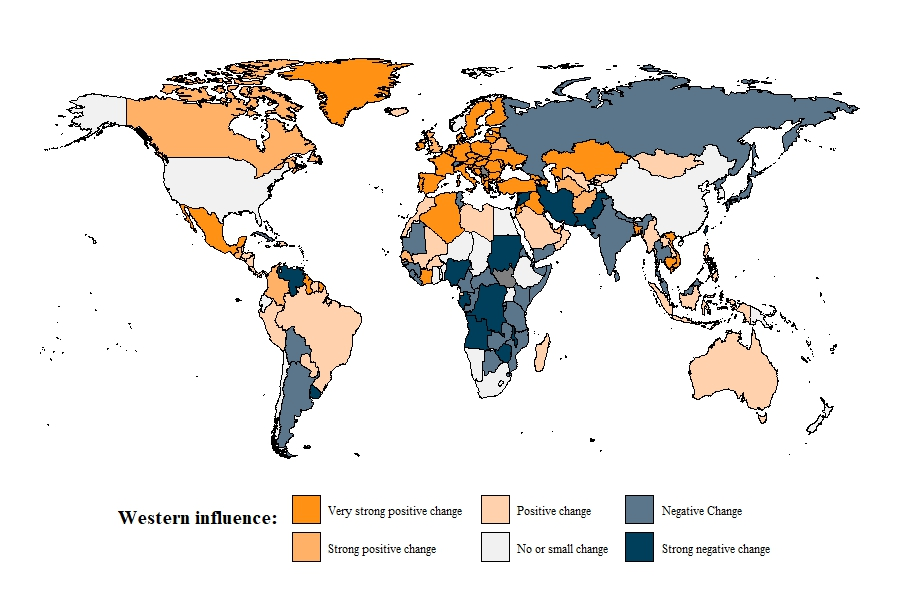
\includegraphics[width = \textwidth]{western_influence.jpeg}
\caption{Change in Western influence}
\label{fig:west}
\end{figure}

Now this is just a speculation on my side, and we need some proof that this is happening. Figure  \ref{fig:west} shows changes in Western\footnote{I have defined the west in this case as any country belonging to the 27 EU countries, as well as all countries with a strong democratic history sins at least the 1990s. The actual countries included in the definition of `The West' can be found in the appendix.} influence for all countries. The orange colour signals a positive change in linkages to the West, while the blue colour signals a negative change. From this we can see that there are some noticeable traces of displacement happening, especially in sub-Saharan Africa. The opposite is true for Europe, where European integration likely has caused Western linkages to strengthen. However there seems to be a trend of China displacing Western ties in some regions of the world, especially sub-Saharan Africa and Central Asia. It would not be unreasonable to think that the change in East-Asia should be far more negative, but the likely reason as to why the West is upholding its position in Southeast Asia is because my definition of the West includes Japan, South Korea, and Taiwan, which are major economic partners to the Southeast Asian countries. 

It is likely that much of the displacement is caused by China's rise as an economic powerhouse. China is the worlds second largest economy, and one of the only great economies that are not Western and democratic. The economic power of China increases China's own heft and norms in the region it displaces Western countries, while at the same time decreasing the power Western countries has to oppose the erosion of freedoms. 

China can also displace Western security linkages. China is the worlds fourth largest arms provider \citep{george_trends_2025, gunter_chinas_2024}, comprising almost six per cent of global exports between 2020 and 2024. However, this is lower than the previous period measured by SIPRI \citep{george_trends_2025}. This decline might down to the fact that China has been rebuilding its military for several years devoting more of its production to domestic use, and Western countries rearming in the face of Russian aggression. The focus on domestic use can perhaps strengthen China as a security partner, a role they are seeking to expand. However, contrary to this, China is a country actively seeking to avoid being entangled in other countries' conflicts, so the only real military alliance China has is with North Korea, showcasing the country's ambivalence to becoming a security guarantor. This makes it doubtful that security linkages are one of the main reasons for displacement, but the fact that China's arms manufacturers have fewer restrictions on whom they sell to \citep{gunter_chinas_2024}, might serve to displace Western influence to some degree.

China is also seeking to displace the West in the realm of diplomacy, to some extent. China has become an important diplomatic partner to many countries, and its position on the UN Security Council makes it Powerful. China has also ambition of creating a more China-centric sphere of influence, sometimes termed the China Model or Beijing Consensus\footnote{The latter as a play on the famous Washington Consensus} \citep{ambrosio_rise_2012, economy_exporting_2020}. This is perhaps most clear in the Shanghai Cooperation Organisation (SCO), which is an international organisation made up of ostensibly authoritarian Central Asian countries, with by far the most powerful country now being China. The organisation is a conservative one, established to preserve the autocratic regimes of the region \citep[p. 1322]{ambrosio_catching_2008}. 

\section{Expectations}
The third wave offers us many cases to study, each of which will be slightly different from all the others. But one of the major changes that has occurred in conjunction with this wave is the rise of China. This is an interesting coincidence, and we should ask the question: are these two phenomena in any way connected?

Previous literature on the subject indicates that we should not expect a concerted effort from China's side to push autocratisation or put pressure on certain freedoms, although this is certainly possible in some cases of particular interest to China, such as Hong Kong \citep{chen_democracy_2015}. We should rather expect to see a gradual change occurring through repeated interaction with China. These interactions are theorised to be measurable through the strength of the linkages between China and other countries.

There is evidence that China really cares about its image abroad and this might influence which countries it gives preference to when it comes to giving aid and preferable loans. However, China also prides itself on its `technocratic' style of government, and we should thus expect China to care more about making the right strategic decisions. These two different goals are quite likely to take place at the same time, and while some countries might get preferential treatment \footnote{There is, however, little evidence of this happening see: \citet{brand_authoritarian_2015}}, we should see a general trend where China forges ties wherever it can.

When China has established the linkages, they begin to have a gradual effect on the partner country's level of freedom of expression. I theorise that there are three main mechanisms through which this effect is channelled: learning, immunity, and favours. the confluence of these factors lead us to the first, and main hypothesis:
\begin{displayquote}
    \textit{H\textsubscript{1}: Thicker linkages to China will have a negative effect on the level of freedom of expression.}  
\end{displayquote}

From previous research \citep{toettoe_foreign_2023}, we know that hybrid regimes are more likely to be affected than other types of regimes. Hybrid, sometimes also known as transitory, regimes are the regimes that show of both democratic and authoritarian characteristics; occupying the centre of the democracy-autocracy spectrum. This gives rise to a secondary hypothesis where hybrid regimes is more likely to be effected by linkages than are consolidated ones. Where electoral autocracies and democracies is likely to be swayed by international pressure, this is less likely to affect closed autocracies and liberal democracies. I reason that this is because the level of freedom of expression is rather set in these societies, and they have robust institutions to handle either attacks or repress freedom of expression. This is not so in hybrid regimes. Hybrid regimes thread a fine line between democracy and autocracy; their regimes usually having a combination of `virtuous' and `perverse' institutions, where democratic and authoritarian characteristics are blended together \citep{valenzuela_democratic_1990}. Hybrid regimes are also more likely to change scores on freedom of expression, because many can be, but are not necessarily, in a transitory phase; either democratising or autocratising.

There is also a ceiling and floor effect at play. on the one hand, liberal democracies cannot increase their level of freedom of expression, because it is almost at the very limit of how unrestricted it can be. On the other hand we find the closed autocracies, where freedom of expression is so low that it cannot reasonably be degraded any further. This leads to secondary hypothesis:
\begin{displayquote}
    \textit{H\textsubscript{2}: Thicker linkages to China will have greater effect on the level of freedom of expression in hybrid regimes.}
\end{displayquote}

These are the two hypotheses I set out to study in the next chapters. The rest of the thesis I dedicate to creating a method of studying these expectations, analysing the results, and discussing what I find. 

\chapter{Research Design} \label{chp:research_design}


\lettrine{H}{having discussed theories} about how our variables are connected, I here construct a research design for testing the implications of my theory. It should be remembered that we are trying to answer if a country's linkages to China affects the level of freedom of expression the population enjoys. To achieve this, it is necessary to have access to good quality data and a credible research strategy.

The first part of the chapter features a discussion of the conceptualisation and operationalisation of our two main variables: \textit{linkages} and \textit{freedom of expression}. I implicitly build this discussion on \citet{adcock_measurement_2001, gerring_what_1999}, who advocates a clear and transparent definition of the variables. Both my main variables are hard to define in a universally accepted manner, which necessitates a thorough explanation of my choices. After discussing the data, the middle part of the chapter will be concerned with the research methodology, specifically how I build the statistical models. This leaves only the end of the chapter; concerning various control-variables which must be incorporated into the model to isolate the actual effect of the linkages from other spurious causes. 

\section{The Dependent Variable: \textit{Freedom of Expression}}
I start by conceptualising and operationalising the dependent variable. There are some challenges to doing this, but the two most important points to take from this section is that: one, my definition of freedom of expression is a nuanced one; and two, that this requires me to use a subjective measure of the variable. The operationalisation will be achieved by using the Varieties of Democracy Institute's (V-Dem) Freedom of Expression and Alternative Sources of Information index \citep{coppedge_v-dem_2025}. 

\subsection{Conceptualising freedom of expression}
Freedom of expression is not at all an easy concept to define in clear terms. Everyone has a basic understanding of the intention: that every person has the right to express their opinion without any obstacles. This is not a wrong, but it quickly gets more opaque when looking at the real world.

Two of the best known definitions are the United Nation's article 19 of the \textit{Universal Declaration of Human Rights} \citeyearpar{un_general_assembly_universal_1948} and the European Union's article 11 of the \textit{Charter of Fundamental Rights of the European Union} \citeyearpar{european_parliament_charter_2012}. The first states that:
\begin{displayquote}
`Everyone has the right to freedom of opinion and expression; this right includes freedom to hold opinions without interference and to seek, receive and impart information and ideas through any media and regardless of frontiers.' \citep{un_general_assembly_universal_1948}
\end{displayquote}
The latter states that:
\begin{displayquote}
`1. Everyone has the right to freedom of expression. This right shall include freedom to hold opinions and to receive and impart information and ideas without interference by public authority and regardless of frontiers.
2. The freedom and pluralism of the media shall be respected.' \citep{european_parliament_charter_2012}
\end{displayquote}
These two are very similar in content, and we can thus read that any definition of freedom of expression should include the possibility of gathering information and imparting information without interference. They also emphasise that access to a pluralistic media environment is important. Affirming that being able to disseminate information to a wide audience factor into our basic understanding of what freedom of expression should be. This is a good start, but we need to be a bit clearer about what type of expressions we are concerned about and what restrictions are and are not proper when defining freedom of expression. 

I include four important limitations to my conceptualisation of freedom of expression. The first limitation I give freedom of expression is that it must be a political expression. Thus, we are not moving into the realm of laws against certain types of pornography \citep[pp. 6-7]{bonotti_freedom_2021} or obscene utterances. Many countries have restrictions on certain types of expressions, which they might have a good reason for having. Of course, if restrictions on non-political expression is used as a tool to silence political expression, they would still qualify as restrictions to political expression.

The second limitation is that the restrictions on freedom of expression must be \textit{de facto} rather than \textit{de jure}. If there are no formal restrictions, but the restrictions of expression still take place, it should count as a restriction of the freedom of expression. On the contrary, if there are legal restrictions, but they are not enforced, e.g., blasphemy laws in western countries, this should not count as a restriction on the freedom of expression. 

The third limitation is that even if the expression is political, restrictions on direct threats and severe forms of libel, should not count negatively for a country's level of freedom of expression. Expressions and actions can in many cases resemble each other, and restrictions on threats and libel to hinder hurt to the object of the expression is not a restriction that imposes itself unduly on the freedom of an actor to expression themself \citep[pp. 81-82]{mill_liberty_2010}. 

The fourth limitation is that certain exceptions should be made. Absolute freedom of expression might on its own be problematic. In the case of Germany there are for instance laws banning expressions of support for Nazism. This is a ban on political expression; however, I would not consider Germany to be repressive because of that. There is context for certain laws, and this should be reflected in the concept, even if we stray from an `ideal.'  

As it stands, our conceptualisation of freedom of expression can be summarised as: \textit{The freedom to express one's  political opinions, and hear others',  without fear of any repercussions from the state, or other actors, and the content should not be a cause of undue hurt to the object.}

\subsection{Operationalising freedom of expression}
The above conceptualisation has important implications for how we operationalise freedom of expression. We have many qualifications, and the second limitation forces us not to rely on a simple count of laws limiting freedom of expression, we are better off using a subjective, rather than an objective, assessment of our variable. Subjective variables come with their own challenges, like inter-coder reliability and systematic bias \citep[for a discussion see:][]{little_measuring_2024, miller_how_2024}, however, the gains by using a more nuanced approach makes it a worthwhile endeavour.

The best and most reliable operationalisation of freedom of expression comes from the V-Dem institute's comprehensive V-Dem dataset \citep{coppedge_v-dem_2025}. The dataset contains many variables and indices used to measure democracy and features relevant to democracy, freedom of expression being a notable one amongst these. The strength of the V-Dem data is that it is thorough, open about its methodology, and includes measures against problems of inter-coder reliability \citep{coppedge_v-dem_2024-2}. (Something about many others using it) There are of course other possible measures to use like Freedom House's \textit{Freedom in the World} dataset \citep{freedom_house_freedom_2024} and the Economist Intelligence Unit's \textit{Democracy Index} \citep{economist_intelligence_unit_democracy_2024}, which both contain variables related to freedom of expression, however, these datasets are hard to disaggregate and have no transparent measures against issues of inter-coder reliability.

Among the variables and indices of the V-Dem dataset we find the Freedom of Expression and Alternative Sources of Information index (henceforth Freedom of Expression index) which we can use as the dependent variable. The variable measures freedom of expression on a theoretical scale from 0 to 1 and answers the question: `\textit{To what extent does government respect press and media freedom, the freedom of ordinary people to discuss political matters at home and in the public sphere, as well as the freedom of academic and cultural expression?}' \citep[pp. 50-51]{coppedge_v-dem_2024-1}. Here 0 denotes a hypothetical country without freedom of expression and 1 denotes a hypothetical country with full freedom of expression. Every real country is somewhere in-between these ideal extremes. In  real terms, the lowest scoring country was North Korea. Between 1994 and 2024 it had a freedom of expression score of 0.012 for every year. The highest scoring country was Denmark in the years from 1994-2010 and 2012-2015 with a score of 0.988.\footnote{Being exactly 0.012 less than 1, this is likely to be an artifact of the aggregation procedure \citep{coppedge_v-dem_2024-2}}. 

\section{The Independent Variable: \textit{Linkages}}
In this section I define and operationalise the independent variable \textit{linkages}. The linkages are conceptualised as a dyadic relationship between countries in some areas of co-operation. They are further divided into the number of linkages and the size of the linkages. Specifically, I use the Formal Bilateral Influence Capacity index (FBIC) developed and compiled by \citet{moyer_china-us_2021}.

\subsection{Conceptualising linkages to China}
Linkages are -- in contrast to freedom of expression -- relatively easy to define. Not only that, it has already been defined for us by the inventors of the concept as used in the field of democratic studies. according to \citet[pp. 383-384]{levitsky_linkage_2006}, linkages can be defined as: `the density of ties and cross-border flows between a particular country and U.S., the EU, and western-dominated multilateral institutions.' \citep[p. 383]{levitsky_linkage_2006} This is a succinct definition, with one glaring problem, I am not interested in links to the West. 

At the most general level, we can define linkages as: \textit{the density of ties and cross-border flows between two countries and their dominant institutions.} This is the most universal conceptualisation of linkages, but for the purposes of this thesis, I can restrict the concept further by including China as the object. This gives us the more differenced concept of linkages.

Thus, linkages to China can be defined as: \textit{the density of ties and cross-border flows between a particular country and China and China-dominated institutions.}

\subsection{Operationalising linkages to China} \label{sec:fbic}
\citet{levitsky_linkage_2006} goes a long way to operationalise the concept of linkages, dividing it in five dimensions. The first dimension is economic, the second is geopolitical, the third is social, the fourth is communication related, and the fourth is society related. I would contend that these can be simplified to three main dimensions: economic, geopolitical, and social, as communication and civil society linkages are closely related to the social and geopolitical linkages. 

To each dimension, \citet{levitsky_linkage_2006} includes several indicators, the aggregate of which can go a long way to measure the width and depth of the linkages. The different indicators is summarised in Table \ref{tab:dimensions}. 

\begin{table}[hbt!]
\centering
\caption{Five dimensions of linkages}
\label{tab:dimensions}
\vspace{0.5em}
\resizebox{\textwidth}{!}{
\begin{tabularx}{\textwidth} {
 >{\noindent\justifying\arraybackslash\hsize=.3\hsize}X 
 >{\noindent\justifying\arraybackslash\hsize=.6\hsize}X
 >{\centering\arraybackslash\hsize=.1\hsize}X}
\toprule
Dimension & Inclusion & FBIC \\
\midrule
Economic linkage
& Trade, investments, credit, and bilateral and multilateral aid flows.
& \checkmark \\
\addlinespace
Geopolitical linkages
& Ties to governments and participations in alliances, treaties, and international organisations
& \checkmark \\
\addlinespace
Social linkages
& Migration, tourism, refugees, diaspora communities, and exchange studies 
& \scalebox{1}[1.5]{$\times$} \\
\addlinespace
Communication linkages
& Cross-border telecommunications, internet connections, and media penetration and coverage 
& \scalebox{1}[1.5]{$\times$} \\
\addlinespace
Transnational civil society linkages
& Local ties to nongovernmental organisations, religious groups, and party organisations
& \scalebox{1}[1.5]{$\times$} \\
\bottomrule
\multicolumn{3}{p{\textwidth}}{\raggedright{\textit{Dimensions are found in \citet[pp. 383-384]{levitsky_linkage_2006}}}}
\end{tabularx}
} % End resizebox
\end{table}

However, there are many linkages, and only some of the data is easily available. I have thus decided to operationalise linkages to China using the Formal Bilateral Influence Capacity index (FBIC), developed by \citet{moyer_china-us_2021}. This is an index that tries to quantify dyadic linkages with a single number. The FBIC index is divided into two parts, bandwidth and dependence, where the former quantifies the extent of the ties and the latter how dependent a country is on another \citep[p. 7]{moyer_china-us_2021}. Dependence is similar to what \citep{levitsky_linkage_2006} terms leverage.

The FBIC index is further divided into three dimensions: economic, security, and political. These correspond most closely to the economic and geopolitical dimensions shown in Table \ref{tab:dimensions} (see column FBIC). The indicators used by Moyer et al. are summarised in Table \ref{tab:fbic} below.

While the FBIC index do lack some of the dimensions and indicators found in \citet{levitsky_linkage_2006}, it is still a good tool for researching the impact linkages have on different countries. Other contributions have already used it to look at how linkages with China might affect media self-censorship \citep{toettoe_foreign_2023}. The main variable of the FBIC is a normalised variable of the weighted variables\footnote{For more information on how the index is calculated, see \citet[pp. 26-31]{moyer_china-us_2021}}, that varies between 0 and 1. 0 means that a country has no influence capacity on another country, and 1 corresponds to the most influence capacity that a country has on another in the dataset \citep[p. 28]{moyer_china-us_2021}. In the real data, the lowest score is 0 for Timor-Leste in 2000. The highest score is that of Pakistan 2023 with an FBIC score of 0.479. 

\begin{table}[H]
\centering
\caption{Components of the FBIC index}
\label{tab:fbic}
\vspace{0.5em}
\resizebox{\textwidth}{!}{
\begin{tabularx}{\textwidth} {
 >{\noindent\justifying\arraybackslash\hsize=.15\hsize}X 
 >{\noindent\justifying\arraybackslash\hsize=.425\hsize}X
 >{\noindent\justifying\arraybackslash\hsize=.425\hsize}X}
\toprule
Dimension & Bandwidth & Dependence \\
\midrule
Economic
& Total goods trade & Goods trade, \% of total \\
& Trade agreements & Goods trade, \% of GDP \\
& & Aid, \% of total aid \\
& & Aid, \% of GDP \\
\\
Security
& Total arms transfers & Arms import stock, \% of total \\
& Military Alliances & Arms import stock, \% of military spending stock \\
\\
Political
& Level of diplomatic representation &  \\
& Shared intergovernmental organisation membership & \\
\bottomrule
\multicolumn{3}{p{\textwidth}}{\raggedright{\textit{Information taken from \citet[p. 7]{moyer_china-us_2021}}}}
\end{tabularx}
} % End resizebox
\end{table}

\section{Observations}
Before diving into the methodology, I would like to summarise the variables and their impact on the research design. First, our unit of analysis---given by our research question---is country-years. In my study I attempt to say something about how different countries change over time,  conditioned on their interactions with China. As the data I am using is gathered on the country-level for each year, it means that my unit of observation will be identical to my unit of analysis. Each row in my data represents a single country in a single year. I include the 174 countries where I have data on the two main variables. In addition, I restrict my sample to the years from 1994 to 2023. The reason for choosing 1994 as a starting point, is because \citet{luhrmann_third_2019} defined this as the starting point of the third wave of autocratisation, and China would not be a relevant actor before this. The end date of 2023 is used because this is the last year I have data on linkage scores. It should be noted that use democracy scores up until 2024,  which avoids losing observations when using a one-year lead on the dependent variable. A list of the countries, as well as the years for which there is data on the variables is included in section \ref{sec:countries} of Appendix \ref{apn:notes}. 

\section{Methodology}
My main objective is to establish if there is -- or is not -- a negative causal relationship between linkages to China and freedom of expression. To achieve this, a sound and transparent methodology is required. In an ideal world, this could have been done by using an experiment, where half the countries would establish linkages with China, and the rest would not. At the same time, I would like to hold all other variables constant, so I knew for sure that the changes that were occurring was caused by the linkages to China.

This is not possible; next to all countries have extensive linkages to China and there are myriads of variables affecting both freedom of expression and linkages with China. However, this little hypothetical is instructive, as it offers an idealised guide to what needs to be controlled for. We first need a treatment: which are countries with different amount of exposure to China. We then need to exclude the possibility of reversed causation, e.g., by either lagging the independent variables or, as I do here, lead the dependent variable. In addition to these methodological steps, I build on the causal mechanisms I established in the previous chapter. Then comes the complicated part where I have to remove the effect of other variables. This is not an easy task, however, by using a fixed effects model and including the control variables described above I attempt to isolate the relationship between linkages to China and freedom of expression.

\subsection{Variable bias}
Excluding variables that cause change in both the dependent and independent variable is a major challenge for inference; therefore I want to spend a little more time talking about how this is done. My research design allows me to control for three distinct types of variables. These are variables that are constant for a unit (country), variables that are constant for a time period (years), and finally, variables that are different across both unit and time. 

The first type of variables to be controlled for, are variables which are different between countries, but stays constant for each country. This can for example be different geographical positions relative to China and different cultural mentalities, both of which could have an impact on both linkages to China and freedom of expression. E.g., a country could be in a region far away from China with a cultural propensity to value freedom of expression. In this case we would expect the country to have few linkages to China and few restrictions on freedom of expression.

The second type of difference to be controlled for are variations across time, but that are common for all the units. One example is economic shocks like the 2008 great economic recession or the corona pandemic. The effect of these shocks might both have led to a global weakening of economic linkages and cause freedom of expression to decline as regimes try to stay in power. Because they affect both of our dependent and independent variables, it is vital for any causal interference that these variables are accounted for when modelling the relationship.

The last type of variation that must be controlled for, is variables that changes both between country and years. I include five additional control variables: GDP per capita, natural resources rents, aid, linkages to the West, and regime type. These are explained in the next section.

\subsection{Fixed effects}
There are many challenges to establish a causal link between two variables. Of course, we would in theory like to follow a process in detail at every stage for every unit. This requires resources of a scale that is next to impossible to attain. However, with data on the results and a solid theoretical foundation, it is possible to say something about complex phenomena. But how can we achieve this?

To resolve the omitted variable problem, I have decided to use a method called fixed effects. In more specific terms I use a two-way fixed effects model controlling for unit and time constants. In very simple terms, fixed-effects is a way to run Ordinary Least Squares (OLS) regression models which accounts for certain observed and unobserved variables. These variables must be constant over a certain dimension, e.g., constant for each country or time period. This is achieved by working with the within variation, rather than the absolute variation, which we have to calculate (\citeauthor{huntington-klein_effect_2022} \citeyear{huntington-klein_effect_2022}; \citeauthor{wooldridge_econometric_2010} \citeyear{wooldridge_econometric_2010}, pp. 301-302).\footnote{This can also be done by using time and unit dummies, which should get you a somewhat similar result, but it is usually easier to work with the within variation \citep{huntington-klein_effect_2022}.} To calculate the within variation, we subtract the mean of the time or unit grouped variables from the individual observations. This process is described below for calculating the within variation for time. 

We start with a regular regression model. Here $y$ is the dependent variable, $x$ represents the vector of independent variables, $c$ is the vector of time-invariant factors (note the absence of the subscript $t$), and $u$ is the error term. The subscripts $i$ and $t$ represents the individual unit and time specific observations respectively. We want to remove the time invariant variables $c$ so that they do not affect our error term. We start by writing the general equation (Equation \ref{equ:within_1})
\begin{equation}
    y_{it} = \beta x_{it} + c_i + u_{it}, \quad i = 1,..., N \quad and \quad  t = 1,..., T  \quad
\label{equ:within_1}
\end{equation} 
To remove the time invariant variables, we then subtract the mean across time of the variables. This is noted by a bar across the variable and the loss of the subscript \textit{t}. This happens for all the variables that change over time. Note that this is not the case for $c_i$, where taking the mean across time by definition makes no difference. Giving us Equation \ref{equ:within_2}:
\begin{equation}
    y_{it} - \bar{y}_i = \beta (x_{it} - \bar{x}_i) + c_i - c_i + u_{it} - \bar{u}_i
\label{equ:within_2}
\end{equation}
Which, when simplifying, is equivalent to Equation \ref{equ:within_3} below. Here the $\ddot{y}_{it}$ is the time demeaned freedom variable, $\ddot{x}_{it}$ represents the time demeaned variables that changes over time, $\ddot{u}_{it}$ is the time demeaned error term, and as can be seen the time invariant variable $c_i$ has completely disappeared. 
\begin{equation}
    \ddot{y}_{it} = \beta \ddot{x}_{it} + \ddot{u}_{it}, \quad i = 1,..., N \quad and \quad  t = 1,..., T  \quad 
\label{equ:within_3}
\end{equation}
We do the same for time as well, however doing them together is a more complicated process and I use an R-package called \textit{fixest} \citep{berge_efficient_2018} to achieve this. This is, however, the basic form of the process, where I try to remove any variable that is fixed for each unit and time period.

\subsection{Control variables} \label{control}
The two-way fixed effects model I use can handle controlling for effects that are fixed over country and year, however, I have to include control variables that changes over both. Using previous research \citep{gamso_is_2021, toettoe_foreign_2023} as a rough guide, I have decided to include five additional variables to reduce the chance of omitted variable bias \citep[pp. 81-85]{wooldridge_econometric_2010}.

The first variable I control for is \textit{GDP per capita}, an important variable which varies both across time, it might rise and fall for the same country, and varies across units, GDP is higher or lower for different countries. Additionally, GDP per capita is argued to be an important variable for the development and retention of democracy \citep{lipset_social_1959, przeworski_modernization_1997}, where freedom of expression is an important component \citep[p. 71]{lipset_social_1959}. There has been a general increase in wealth from the early 1990s, but at different rates and countries start from a different baseline. Thus, not controlling for GDP per capita could lead us to make wrong inferences. GDP per capita also impact linkages, with richer countries having more capacity to trade and engaging in diplomacy. (!CITE!) The variable is constructed by taking the average GDP per capita as measured by the \citet{world_bank_world_2025}, the \citet{imf_world_2025}, and the \citet{united_nations_statistics_division_national_2025}. Since the distribution of GDP per capita is very skewed, I have decided to use the log-transformed variable, giving me a continuous variable between 4.37 and 11.81. 

The second control variable is \textit{total natural resources rents}. This variable varies greatly between countries, some having abundant resources, others not; and over time, since prices on natural resources varies after economic condition and the resources might deplete. Rents from natural resources might have several possible effects on freedom of expression. Most of the discussion centred around the impact of natural resources is focused on democracy and autocracy, but I consider the effect to be the same on freedom of expression \citep{lipset_social_1959}. On the one hand, some have argued that natural resources have a positive effect on democracy \citep{brooks_oil_2016, haber_natural_2011}. Getting a windfall from natural resources might, for instance, make citizens richer, leading them to demand more rights and participation in society \citep{brooks_oil_2016, lipset_social_1959}. On the other hand, some argue that natural resources might lead to autocratisation (\citeauthor{andersen_big_2014} \citeyear{andersen_big_2014}; \citeauthor{brooks_oil_2016} \citeyear{brooks_oil_2016}, pp. 281-285). E.g., authoritarian regimes in resource rich countries might be able to keep in power by using the resource rents to bribe or repress the population \citep[p. 282]{brooks_oil_2016}. The effect on linkages would be that resource rich countries export their resources, thus facilitating both economic and diplomatic ties. I use the World Bank's World Development Indicators (WDI) measure of total natural resources rents \citet{world_bank_world_2025}, which measures natural resource rents in per cent of GDP. This variable varies between 0 and 88.59. 

The third variable is Official Development Assistance (ODA), more commonly known as \textit{aid}. I expect Aid to be similar to rents, as it might help the government stay in power as it can buy of the citizenry. However, it might also increase living standards, making citizens more likely to demand participation in government. The scholarship on the subject is, however, divided. Some find a negative effect \citep{djankov_curse_2008}; others no relationship \citep{altincekic_why_2014}. While aid might function like natural resources \citep{djankov_curse_2008}, \citet[p. 30]{altincekic_why_2014} argues that aid is too volatile to be able to prop up authoritarian regimes. I include it as it might be able to obscure the effect of linkages to China, as it is a source of revenue, which might offset some of China's impact. Aid varies over time, after how much a country needs the aid, and between countries, as only some countries need aid at all. Observant readers might already have noted that my variable measuring linkages to China includes aid as one of the components. This is not good as this might cause collinearity between the variables. However, I have gathered data on aid from the OECD \citep{oecd_dac2a_2025}, which only include aid from donors on or associated with the Development Assistance Committee (DAC), to which China has no association \citep{oecd_development_2025}. When a country receives aid it creates ties to foreign countries which the receiving country might build upon to reach out to other countries again. It might also help to maintain an export industry in the face of economic problems, helping to keep linkages from falling away. The aid variable is measured as per cent of Gross National Income (GNI) and is a continuous variable between 0 and 113.13. 

The fourth control variable measures the impact of a country's \textit{linkages to the West}. The whole theory of linkages is developed from the point of view that linkages to Western countries can aid democratisation \citep{levitsky_linkage_2006}. It is not far-fetched, then, to think that these linkages may serve to strengthen freedom of expression. Linkages to Western varies over time and country, and if unaccounted for might obscure the effect of the Chinese linkages. When a country increases its linkages to the West, linkages to China might decrease, and vice versa. It is therefore an important variable to control for. The linkage variable to the West is the sum of the FBIC-score of all `Western' countries. I define Western countries as any Western European country, any country with strong inheritance from Western European countries (like the US) and any democratic and strongly Western aligned country (e.g., Japan).\footnote{I include a list of the countries that make up the linkages to the West variable in Appendix \ref{apn:notes}.} The measure is a continuous variable which varies between 0.03 and 5.32. Here 0 means zero influence and 5.32 is the highest recorded influence in the restricted dataset (1994-2023). 

The fifth and final variable is \textit{regime type}. Regime type is added for two main reasons. One is that regime type is another variable that changes both across time and country. The difference between countries is obvious, some are autocracies, while others are democracies. However, they might change over time, either becoming more or less democratic. The second reason is to enquire into our second hypothesis (\textit{H\textsubscript{2}}), to see if there are differences between regime types in how linkages affect freedom of expression. To measure regime type, I use the Regimes of the World variable included in the V-Dem dataset \citep{coppedge_v-dem_2025}. This is an ordinal variable of four levels between 0 and 3, where 0 represents a closed autocracy, 1 represents an electoral autocracy, 2 represents an electoral democracy, and 3 represents a liberal democracy. One consideration to make is that the freedom of expression variable goes into constructing this variable. However, this should not be a problem as this is more akin to an indexing variable. In Table \ref{tab:summary} I have included summary statistics for all my variables.

\begin{table}[H]
\centering
\caption{Summary statistics}
\label{tab:summary}
\vspace{0.5em}
\begin{tblr}[         %% tabularray outer open
]                     %% tabularray outer close
{                     %% tabularray inner open
colspec={Q[]Q[]Q[]Q[]Q[]Q[]Q[]Q[]},
column{1}={}{halign=l,},
column{2,3,4,5,6,7,8}={}{halign=r,},
}                     %% tabularray inner close
\toprule
& N & Mean & Median & SD & Min & Max & Density \\ \midrule %% TinyTableHeader
Freedom & 5368 & 0.66 & 0.75 & 0.29 & 0.01 & 0.99 & 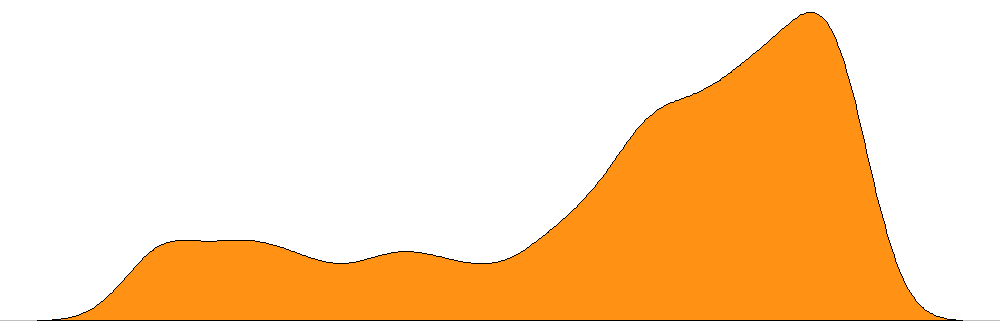
\includegraphics[height=1em]{tinytable_assets/idkw3ss7dtaehv6mshzwwl.png} \\
Linkages to China & 5154 & 0.08 & 0.05 & 0.08 & 0.00 & 0.48 & 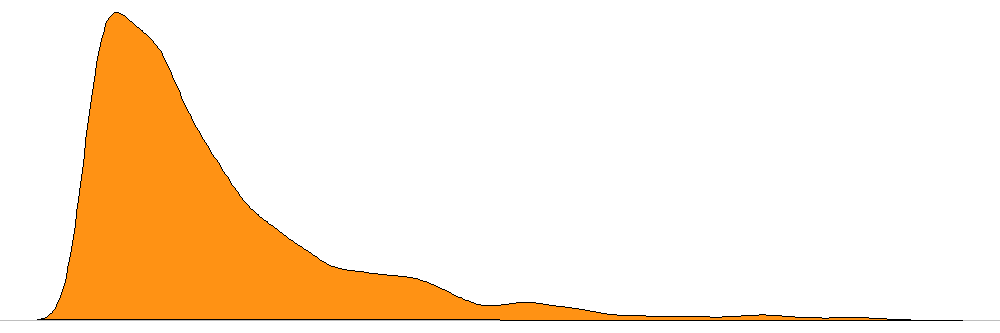
\includegraphics[height=1em]{tinytable_assets/idgbl0sn5x5im94irfzhyq.png} \\
GDP per capita & 5190 & 8.20 & 8.16 & 1.58 & 4.37 & 11.81 & 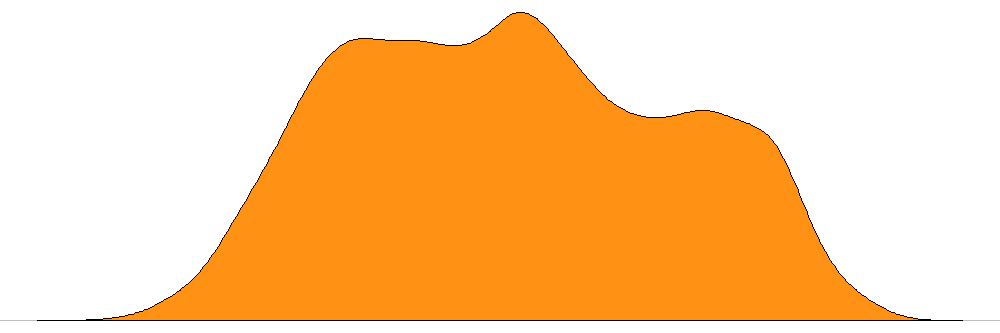
\includegraphics[height=1em]{tinytable_assets/iduvca3az1vb55iagqjao4.png} \\
Natural resources & 4679 & 7.74 & 2.68 & 11.35 & 0.00 & 88.59 & 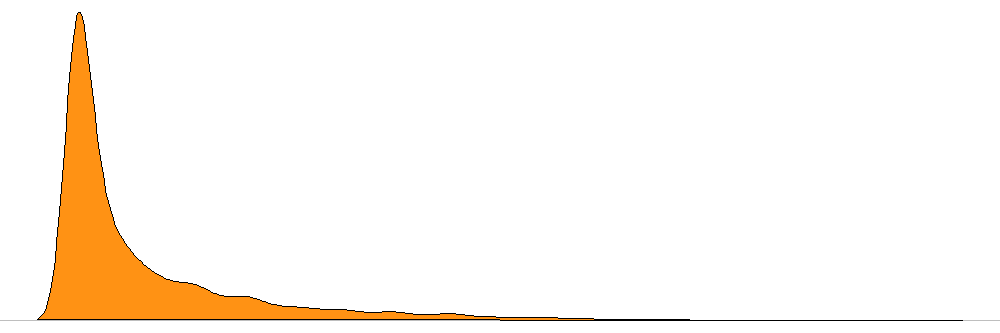
\includegraphics[height=1em]{tinytable_assets/id2fj7dkybom42ciuf8nxw.png} \\
Aid & 5213 & 4.25 & 0.78 & 8.01 & 0.00 & 113.13 & 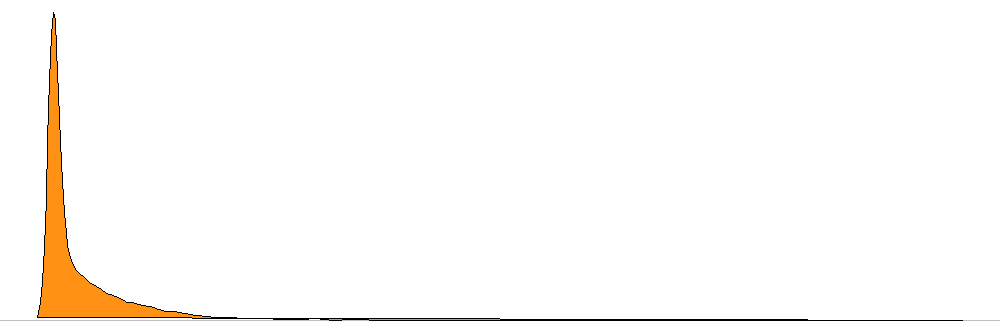
\includegraphics[height=1em]{tinytable_assets/idsk9x35wnd8lbeg36z6ir.png} \\
Linkages to the West & 5154 & 1.08 & 0.68 & 1.08 & 0.03 & 5.32 & 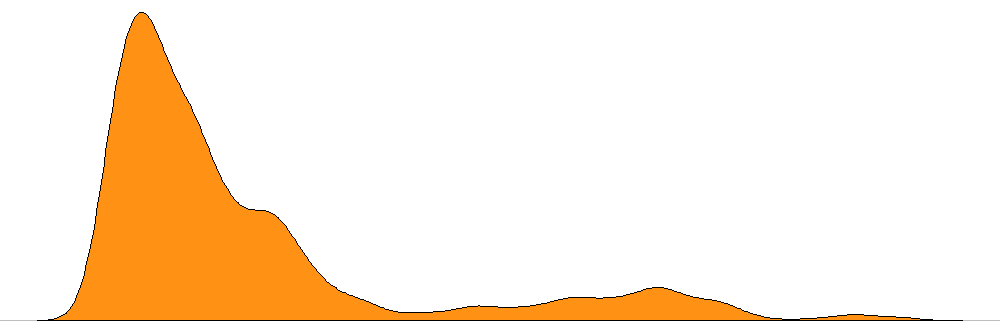
\includegraphics[height=1em]{tinytable_assets/id0blqnye1aky5vllx8gn6.png} \\
Regime & 5368 & 1.59 & 2.00 & 1.00 & 0.00 & 3.00 & 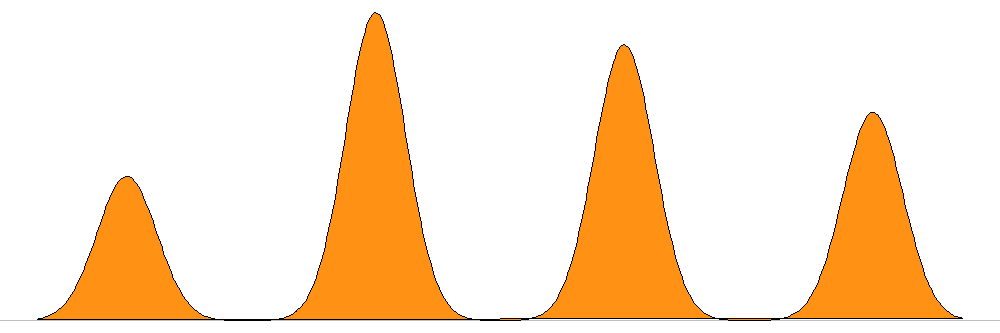
\includegraphics[height=1em]{tinytable_assets/idtplecxtx0acvwxi990hv.png} \\
\bottomrule
\end{tblr}
\end{table} 

\subsection{Challenges to inference}
While fixed effects solves many inference problems by removing time and unit constants, reducing unobserved variable bias. However, it is far from a panacea, and we need to be conscious of this fact. The first problem with using fixed effects is that there can still be \textit{unobserved heterogeneity} (\citeauthor{cunningham_causal_2021} \citeyear{cunningham_causal_2021}, Chapter 8, \citeauthor{hill_limitations_2020} \citeyear{hill_limitations_2020}, pp. 363-364). These are variable that vary across both unit and time. I try to account for this heterogeneity by including control variables, but there will always be a possibility that there is some unobserved heterogeneity; a risk that can only be mitigated to the best of one's ability.

A second challenge is that fixed-effects modelling can have \textit{low statistical power} \citep[pp. 361-362]{hill_limitations_2020}. Taking the within variation might limit information and this makes estimation harder. My linkage variable has a mean of 0.08, which is quite small. So, this could be a challenge. I still consider there to be enough variation to be useful, but this is something to keep in mind.

The last major concern of fixed-effects is that \textit{coefficients are harder to interpret} \citep[pp. 364-365]{hill_limitations_2020}. This is especially so for the two-way fixed effect model I use here. To try to make it easier for the reader I will use examples, to show how the coefficients might be interpreted.

\subsection{The models}
Fixed effects solve the problem where variables that are fixed over time and country influences the results. The last hurdle is to remove effects caused by variables that varies over both time and units. To do this I include the controls for GDP per capita, natural resources rents, aid, and linkages to the West. Including these should remove any spurious effects that might cause bias when estimating the relationship between linkages to China and freedom of expression. The final models are represented in the two equations below.
\begin{align} \label{equ:h1}
    freedom_{it+1} =\, & \beta_1  linkages_{it} + \beta_2 log(gdppc)_{it} + \beta_3 rents_{it} + \beta_4aid_{it} + \nonumber\\
    & \beta_5 west_{it} + \beta_6  factor(regime)_{it} + \chi_1 country_t + \chi_2 time_i + \epsilon_{it}
\end{align}
In Equation \ref{equ:h1} the freedom of expression variable with a one-year lead is a function of  linkages to China, the log-transformed GDP per capita, rents, aid, linkages to the west, regime type, and an error term.

When working with hypotheses two, we need a slightly different model from the one above. Instead of including the regime variable as an independent term, we furnish the models with an interaction term between the linkage variable and the factorised regime variable. This makes it possible to see the effect of linkages on different regime types. The interaction model is shown in Equation \ref{equ:h2}:
\begin{align} \label{equ:h2}
    freedom_{it+1} =\, & \beta_1 linkages_{it} + \beta_2 factor(regime)_{it} + \beta_2 log(gdppc)_{it} + \beta_3 rents_{it} + \nonumber\\
    & \beta_4 aid_{it} + \beta_5 west_{it} + \beta_6 (linkages * factor(regime)) + \nonumber\\
    & \chi_1 country_t +\chi_2 time_i + \epsilon_{it}
\end{align}

\chapter{Analysis} \label{chp:analysis}
\lettrine{I}{n this chapter I present} the results of the models that have been specified in the previous chapter. What I find is that there is no evidence that linkages to China is influencing the level of freedom of expression in a country. This result does not change even when considering different types of regimes, which I theorised might behave differently when developing stronger links to China. This result is stable across different specifications. The one exemption is that I found a strong negative effect on hybrid regimes with a ten-year lead on the dependent variable. This is not directly implausible, but I consider the time span and variation in the data to too great, making this a spurious relationship. 

I start this chapter by giving a few examples of how linkages to China and freedom of expression have co-varied over the time span in consideration (1994-2023).  This is a descriptive exercise to see if the theory is plausible. After this I turn to the results of the model estimations. I present and explaining how the results might be interpreted, noting some of the more interesting details. This chapter ends with a discussion on the validity, reliability, and the robustness of the results, as there are many ways in which to model data, and even small changes may have large impacts on the results.

\section{Examples}
\begin{table}[!hbt]
\centering
\caption{Changes in freedom of expression and linkages to China}
\label{tab:change}
\vspace{0.5em}
\begin{tabular}{lLp{15mm}lL}
\toprule
Country & \multicolumn{1}{c}{Freedom} & & Country & \multicolumn{1}{c}{Linkage} \\
\midrule
\cellcolor[HTML]{ff9214} Timor-Leste & 0.776 & & 
\cellcolor[HTML]{ff9214} Cambodia & 0.394 \\
Maldives & 0.636 & & Laos & 0.326 \\
Tunisia & 0.533 & & Turkmenistan & 0.314 \\
Libya & 0.531 & & Malaysia & 0.302 \\
Iraq & 0.510 & & Angola & 0.924 \\
\addlinespace
Hong Kong & -0.568 & & Tunisia & 0.018 \\
Venezuela & -0.670 & & Romania & -0.031 \\
Belarus & -0.735 & & Iran & -0.034 \\
Russia & -0.735 & & The Gambia & -0.067 \\
\cellcolor[HTML]{003F5C}\textcolor{white}{Nicaragua} & -0.869 &  &
\cellcolor[HTML]{003F5C}\textcolor{white}{North Korea} & -0.201 \\
\bottomrule
\multicolumn{5}{p{0.7\textwidth}}{\raggedright{\textit{For freedom score the the difference is measured between 1994 and 2024 \citep{coppedge_v-dem_2025}, while for linkage score it is the difference between 1994 and 2023 \citep{moyer_china-us_2021}.}}}
\end{tabular}
\end{table}

I want to start this section by examining some countries in greater detail to look at how our dependent and independent variables have changed over the time frame we are looking at. For freedom of expression, I have data from 1994 to 2024 and for linkages to China, I have data from 1994 to 2023. 

Are there any signs that the main hypothesis is true? I have chosen four countries, based on their scores on the two main variables. These are: Timor-Leste, with the largest increase in freedom of expression score; Nicaragua, with the largest decrease in freedom of expression score; Cambodia, with the largest increase in linkages with China; and North Korea, with the largest decrease in linkages with China. The top and bottom five of both dependent and independent variables can be seen in Table \ref{tab:change}.

\begin{figure}[!hbt]
    \centering
    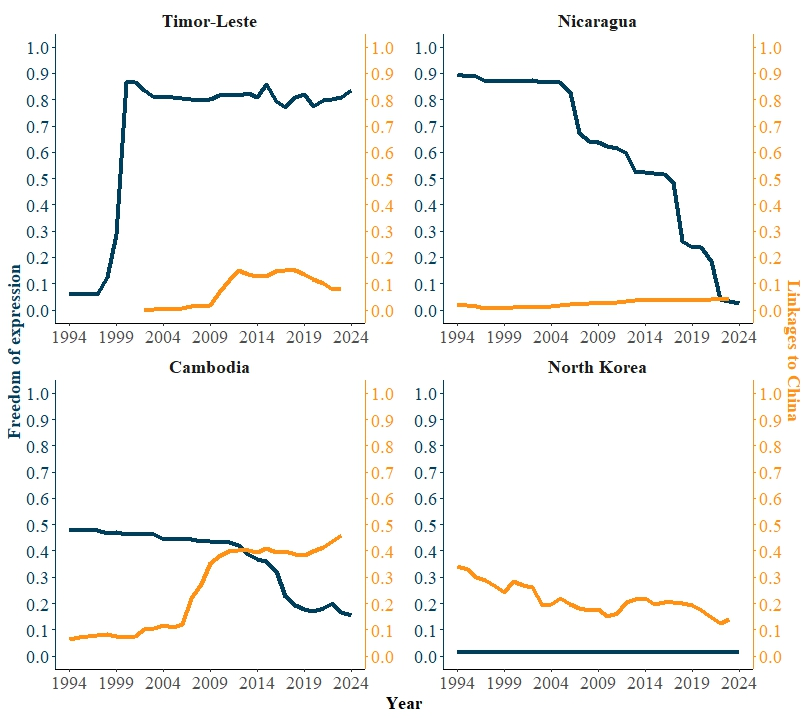
\includegraphics[width=\linewidth]{graphics/single_country_plots.jpeg}
    \caption{Change in linkages to China and freedom of expression (1994-2023/4)}
    \label{fig:scp}
\end{figure}


\subsection{Timor-Leste}
Timor-Leste, also known as East Timor, is a small country in Southeast Asia, located on the east part of the island of Timor, which it shares with its larger neighbour Indonesia. The country has had a fraught history, that reached its climax in 1999, when the country became independent from Indonesia after 24 years of occupation \citep[p. 183]{kingsbury_democratic_2014}. In Figure \ref{fig:scp} we can see that there is a large jump in the freedom of expression score in 1999, going from a score as low as 0.06 in 1997 to reaching a high of 0.87 in 2000. After which the score has held relatively stable. While the FBIC index do not include scores for Timor-Leste before 2002, linkages to China only began rising around 2010, but this has not seemed to impact freedom of expression to any significant degree.

In the case of Timor-Leste, it is independence from Indonesia which facilitated the rapid increase in freedom of expression. This is to highlight that, while linkages to China might have an effect, they can easily be drowned out by the noise of domestic realities, or at least problems much closer to home.

\subsection{Nicaragua}
Nicaragua is a poor Central American country, with a turbulent modern history, which shows in the decline of freedom of expression in the country. Since 2006, freedom of expression has declined rapidly under the leadership of Daniel Ortega, who, colluding with the opposition president, from 2000 gradually managed to gain more and more power, essentially being able to effect executive aggrandisement from a minority position \citep{mcconnell_elite_2024}.

While linkages to China have slowly increased between 1994 and 2023, this has happened at a very slow pace, and in absolute numbers they are very low. The reason for this is that Nicaragua has long recognised Taiwan as being the official China, to which China is not amicably disposed. This state of affairs, however, ended in 2021 when the country broke of diplomatic contact with the island nation \citep{bbc_nicaragua_2021}. Nicaragua's recognition of Taiwan has long limited relations with China, but I expect that the change of recognition will cause linkages between China and Nicaragua to expand dramatically in the future. However, as this is a recent development, this has not had the time to appear in the data. 

China most likely does not have much impact on Nicaragua, but this might not mean that linkages are not in play, just not linkages to China. \citet[p. 198]{mcconnell_elite_2024} argues that Black Knight authoritarian allies have had a great deal of influence, with Venezuela taking the lead. At the same time, she emphasises domestic elite explanations, where the Black Knights are ancillary to domestic processes.

\subsection{Cambodia}
Cambodia is a country on the Indochinese peninsula, which was not spared the ravages of the Cold War, hosting one of the most brutal regimes the world has ever seen in the communist Khmer Rouge. It did subsequently democratise; however, this was never very successful, quickly becoming more authoritarian. In this autocratisation process freedom of expression has taken a large hit. At first this process was slow, with the country recording a slow but persistent decline in freedom of expression in the period between 1994 and 2012. This changed in 2012 as the score declined rapidly, before re-stabilising at a low level.

It is telling that the repression on freedom of expression began in earnest after a rapid increase in ties to China. The two lines in Figure \ref{fig:scp} seem almost to mirror each other, giving, at least a superficial impression, that there is a connection. This is substantiated by \citet{loughlin_chinese_2021}, who finds that the ruling Cambodian People's Party (CPP) has been both learning from and supported itself on China

\subsection{North Korea}
The last country I want to look at is North Korea, commonly labelled the hermit kingdom for its super-authoritarian and repressive regime. Its system is founded on self-reliance or Juche, with a strong cult of personality surrounding the ruling Kim clan. North Korea occupies the northern half of the Korean peninsula and is almost entirely reliant on support from China as it faces crushing sanctions from the West. However, after the Russian invasion of Ukraine in 2022 Russia has become a much closer partner.

We see from the blue line in Figure \ref{fig:scp} that freedom of expression in North Korea is non-existent. North Korea is probably the most repressive regime on earth and there is no freedom to be had for a citizen. This has not changed even slightly in the last thirty years. The yellow line shows North Korea's linkages to China. This has fallen in recent years, which might either be because North Korea is diversifying its foreign policy or that China has become less eager to engage with the country, especially from 2006 when Pyongyang conducted its first nuclear weapons test \citep{fong_understanding_2024}. Whatever the case, the weakening of linkages to China in this period seems to have had no effect on freedom of expression in North Korea.

\section{Statistical Significance}
Before proceeding with the analysis, I will make a quick rejoinder on statistical significance. The reason is that I will refer to statistical significance as a convention. However, significance is an arbitrarily chosen threshold; being the point where we consider a result to be plausible enough that we reject the null-hypothesis and accept the results as being `true.' The most accepted threshold goes at the five per cent level (\citeauthor{christophersen_introduksjon_2018} \citeyear{christophersen_introduksjon_2018}, pp. 27-31; \citeauthor{gelman_regression_2021} \citeauthor{gelman_regression_2021}, p. 57; \citeauthor{halperin_political_2020} \citeyear{halperin_political_2020},  p. 432; \citeauthor{hellevik_forskningsmetode_2002} \citeyear{hellevik_forskningsmetode_2002}, p. 375; \citeauthor{kellstedt_fundamentals_2018} \citeyear{kellstedt_fundamentals_2018}, pp. 165-166), meaning that if we do the study 100 times, we can expect that in 95 of them of them we end up with a coefficient that is different from zero, and we can plausibly reject the null-hypothesis.

There is a tendency in the statistical community to be over-reliant on significance testing \citep{barnett_examination_2019, gelman_regression_2021, imbens_statistical_2021, van_zwet_significance_2021}. This is a problem as it incentivises researchers to aim for statistical significance, to the detriment of gaining true insight. We should therefore not be too concerned about significance but use it as a rough way to distinguish the probable from the improbable.

When considering significance, it is important to be aware of two points: one is that the effect should be large enough to be of consequence and the other is that there are enough observations. I will be discussing effect size later, especially in Section \ref{sec:effect}. My models vary between 5,154 and 3,473 observations. This is a fair number of observations, but in some cases, especially when adding an interaction term of a four-levelled factor variable (Table \ref{tab:h2}), it might not be enough to get a significant result, even if there is an effect. This is important to have in mind when trying to make sense of the results.

\section{Hypothesis One} \label{sec:h1}
In this section and the next, I present the results of the first regression model from the research design chapter, where I gradually include controls to test the stability of the results (Table \ref{tab:h1}). As a quick reminder, hypothesis one states that: \textit{thicker linkages to China will have a negative effect on the level of freedom of expression.} In addition to Table \ref{tab:h1}, I also include a table showing the fully specified model with different amounts of lead on the dependent variable (Table \ref{tab:h1_lead}). I do this to enquire into whether or not there is a time delay to the linkages. All models use two-way fixed effects to control for country and time invariables, as this is likely to be a source of unobserved variable bias if they remain uncontrolled for. Because there is a high likelihood that there are considerable differences in the standard errors of the units, I cluster the standard errors by country, making them robust to unit heterogeneity. For readability, I have also decided to highlight the linkages to China variable in the regression tables. It will be orange if there are no significant finds, and blue if the coefficients are significant at the five per cent level. This should, however, only be thought of as a reading aid. 

\subsection{Relationship between linkages to China and freedom of expression}
\begin{table}[H]
\centering
\resizebox{\textwidth}{!}{
\begin{talltblr}[         %% tabularray outer open
label=tab:h1,caption={Standard two-way fixed-effects models},
note{}={x p \num{< 0.1}, * p \num{< 0.05}, ** p \num{< 0.01}, *** p \num{< 0.001}},
]                     %% tabularray outer close
{                     %% tabularray inner open
colspec={Q[]Q[]Q[]Q[]Q[]Q[]Q[]},
column{2,3,4,5,6,7}={}{halign=c,},
column{1}={}{halign=l,},
hline{18}={1,2,3,4,5,6,7}{solid, black, 0.05em},
}                     %% tabularray inner close
\toprule
& \textbf{Model 1.1} & \textbf{Model 1.2} & \textbf{Model 1.3} & \textbf{Model 1.4} & \textbf{Model 1.5} & \textbf{Model 1.6} \\ \midrule %% TinyTableHeader
\SetCell{bg=Orange} Linkages to China &
\SetCell{bg=Orange} -0.081 & 
\SetCell{bg=Orange} -0.093 & 
\SetCell{bg=Orange} -0.069 & 
\SetCell{bg=Orange} -0.067 & 
\SetCell{bg=Orange} -0.111 & 
\SetCell{bg=Orange} -0.058 \\
& (0.132) & (0.134) & (0.127) & (0.128) & (0.130) & (0.111) \\
log(GDP per capita) &  & 0.009 & 0.001 & 0.008 & 0.016 & -0.003 \\
&  & (0.019) & (0.020) & (0.022) & (0.023) & (0.020) \\
Resource rents &  &  & 0.000 & 0.000 & 0.000 & 0.000 \\
&  &  & (0.001) & (0.001) & (0.001) & (0.001) \\
Aid &  &  &  & 0.001 & 0.001 & 0.002** \\
&  &  &  & (0.001) & (0.001) & (0.001) \\
Linkages (West) &  &  &  &  & -0.023* & -0.016x \\
&  &  &  &  & (0.012) & (0.009) \\
Electoral autocracy &  &  &  &  &  & 0.085** \\
&  &  &  &  &  & (0.030) \\
Electoral democracy &  &  &  &  &  & 0.238*** \\
&  &  &  &  &  & (0.034) \\
Liberal democracy &  &  &  &  &  & 0.285*** \\
&  &  &  &  &  & (0.037) \\
Num.Obs. & 5154 & 5150 & 4657 & 4648 & 4648 & 4648 \\
Std.Errors & by: country & by: country & by: country & by: country & by: country & by: country \\
R2 Adj. & 0.874 & 0.874 & 0.882 & 0.883 & 0.883 & 0.907 \\
R2 Within Adj. & 0.001 & 0.001 & 0.000 & 0.003 & 0.008 & 0.208 \\
FE: country & X & X & X & X & X & X \\
FE: year & X & X & X & X & X & X \\
\bottomrule
\end{talltblr}
}
\end{table} 

Table \ref{tab:h1} includes six different versions of Model 1, estimating the effect of linkages to China on freedom of expression. Model 1.6, the most complex, is equivalent to Equation \ref{equ:h1} above. Model 1.1 regress linkages to China directly on freedom of expression without including any control variables. I then gradually include the five control variables described in Section \ref{control}. The first control variable I include is the logged GDP per capita variable (Model 1.2), the second is total natural resources rents as a percentage of GDP (Model 1.3), the third is Official Development Assistance, better known as aid, which is measured as per cent of GNI (Model 1.4), the fifth is linkages to the West, an aggregate of linkages to Western countries (Model 1.5), and the final model introduces the regime control variable, a factor variable of four levels, with closed autocracies being the reference value (Model 1.6), giving us the full model.  I start with 5,154 observations, and in the last model I end up with 4,648, losing 506 observations through missingness on the control variables. The biggest loss of observations happens when including the total natural resources rents variable in model 1.3, because this variable only has data up until 2021. All the models are all using country and time fixed effects, with the freedom of expression scores being led by one year to exclude reversed causation. 

The highlighted row labelled Linkages to China shows us the main effect we are after, namely the effect of linkages to China on freedom of expression. The sign of this coefficient is negative in all cases, indicating that linkages to China have a negative effect on freedom of expression. However, we see that the effect sizes are small, and the standard errors are large, so we cannot be confident in this relationship. Other than this, there are a few more things to note. First, the coefficient for GDP per capita is non-significant and small, probably indicating that most of the variation in this variable is controlled for by using fixed effects. Second, that aid is significant only when also controlling for regime type. Third, that linkages to the West is negative and statistically significant in Model 1.5, but the significance disappears when controlling for regime type. This is very surprising in light of earlier studies \citep{levitsky_linkage_2006}, however, I will explore this further below in the discussion chapter. And fourth, that regime type is always positive and statistically significant. This latter observation is unsurprising as one, all the regime types are more democratic than the reference regime type, which is closed autocracy, and two, because the regime variable is partially based on the freedom of expression variable.

It can be clearly seen in Table \ref{tab:h1} that linkages to China does not have a direct impact on freedom of expression scores. While the sign of the linkage variable is indeed negative, the standard error is quite large, being more than twice the size of the estimated effect in all models.

\subsection{Different time leads}
I also test how the model reacts when using different time leads. I do this by using the most complex model from Table \ref{tab:h1} (Model 1.6). I test for five additional time leads in Table \ref{tab:h1_lead}, starting with a lead of two years in Model 1.7, four in Model 1.8, six in Model 1.9, eight in Model 1.10, and finally ten in Model 1.11. From the example of Cambodia in Figure \ref{fig:scp}, it seems like linkages take time before they have an effect, and this is an important exercise to examine this relationship further.

The size of the coefficient for linkages to China increases up until an eight-year lead, before it decreases again. The sign is negative, and the effect becomes somewhat sizeable. However, the standard error is still large and never reaches the five per cent threshold of statistical significance, meaning that we should consider it implausible that linkages to China have an effect on freedom of expression. 

What is more interesting to see is that linkages to the West is negative and statistically significant for all leads. It means that if a country increases its linkages to the West, the model predicts that freedom of expression decreases. We should also note that the regime factor variables all lose significance and coefficient size. This is expected as the further removed from the freedom of expression score in time, the less they should be able to predict it. 

\begin{table}[H]
\centering
\resizebox{\textwidth}{!}{
\begin{talltblr}[         %% tabularray outer open
label=tab:h1_lead,caption={Model 1.6 with different leads},
note{}={x p \num{< 0.1}, * p \num{< 0.05}, ** p \num{< 0.01}, *** p \num{< 0.001}},
]                     %% tabularray outer close
{                     %% tabularray inner open
colspec={Q[]Q[]Q[]Q[]Q[]Q[]},
column{2,3,4,5,6}={}{halign=c,},
column{1}={}{halign=l,},
hline{18}={1,2,3,4,5,6}{solid, black, 0.05em},
}                     %% tabularray inner close
\toprule
& \textbf{Model 1.7} & \textbf{Model 1.8} & \textbf{Model 1.9} & \textbf{Model 1.10} & \textbf{Model 1.11} \\ \midrule %% TinyTableHeader
\SetCell{bg=Orange} Linkages to China &
\SetCell{bg=Orange} -0.088 & 
\SetCell{bg=Orange} -0.188 & 
\SetCell{bg=Orange} -0.278x & 
\SetCell{bg=Orange} -0.318x & 
\SetCell{bg=Orange} -0.272 \\
& (0.118) & (0.137) & (0.156) & (0.175) & (0.184) \\
log(GDP per capita) & 0.003 & 0.013 & 0.017 & 0.012 & 0.001 \\
& (0.020) & (0.022) & (0.021) & (0.017) & (0.016) \\
Resource rents & 0.000 & 0.000 & 0.000 & 0.000 & 0.000 \\
& (0.001) & (0.001) & (0.001) & (0.001) & (0.001) \\
Aid & 0.002* & 0.001 & 0.001 & 0.000 & 0.000 \\
& (0.001) & (0.001) & (0.001) & (0.001) & (0.001) \\
Linkages (West) & -0.020* & -0.027* & -0.031* & -0.034* & -0.035* \\
& (0.009) & (0.011) & (0.012) & (0.013) & (0.014) \\
Electoral autocracy & 0.063* & 0.028 & 0.008 & 0.002 & -0.015 \\
& (0.028) & (0.026) & (0.025) & (0.024) & (0.026) \\
Electoral democracy & 0.192*** & 0.112*** & 0.061* & 0.037 & 0.017 \\
& (0.032) & (0.029) & (0.027) & (0.026) & (0.029) \\
Liberal democracy & 0.241*** & 0.165*** & 0.112** & 0.081* & 0.059x \\
& (0.035) & (0.034) & (0.035) & (0.034) & (0.034) \\
Num.Obs. & 4648 & 4484 & 4149 & 3812 & 3473 \\
Std.Errors & by: country & by: country & by: country & by: country & by: country \\
R2 Adj. & 0.899 & 0.894 & 0.897 & 0.899 & 0.903 \\
R2 Within Adj. & 0.149 & 0.073 & 0.042 & 0.030 & 0.026 \\
FE: country & X & X & X & X & X \\
FE: year & X & X & X & X & X \\
Lead freedom & 2 & 4 & 6 & 8 & 10 \\
\bottomrule
\end{talltblr}
}
\end{table} 

\section{Hypothesis Two} \label{sec:h2}
In hypothesis two, I set out to study if the effect of linkages to China is regime dependent. It will be remembered from the last chapter of the theory section that hypothesis two states: \textit{Thicker linkages to China will have a greater negative effect on the level of freedom of expression in hybrid regimes}. To assess the veracity of this hypothesis, I add an interaction term between the linkages to China variable and the regime variable. The resulting interactions show the effect of linkages on a certain type of regime, with closed autocracies being the reference category. For the purposes of hypothesis two, I consider closed autocracies and liberal democracies to be `institutionalised regimes,' while electoral autocracies and democracies are considered hybrid regimes. All the other specifications are similar to hypothesis one. 

\subsection{Relationship between linkages to China and freedom of expression by regime type}

\begin{table}[!hbt]
\centering
\resizebox{\textwidth}{!}{
\begin{talltblr}[         %% tabularray outer open
label=tab:h2,caption={Relationship between linkages to China and freedom of expression including regime type interaction},
note{}={x p \num{< 0.1}, * p \num{< 0.05}, ** p \num{< 0.01}, *** p \num{< 0.001}},
]                     %% tabularray outer close
{                     %% tabularray inner open
colspec={Q[]Q[]Q[]Q[]Q[]Q[]},
column{2,3,4,5,6}={}{halign=c,},
column{1}={}{halign=l,},
hline{24}={1,2,3,4,5,6}{solid, black, 0.05em},
}                     %% tabularray inner close
\toprule
& \textbf{Model 2.1} & \textbf{Model 2.2} & \textbf{Model 2.3} & \textbf{Model 2.4} & \textbf{Model 2.5} \\ \midrule %% TinyTableHeader
\SetCell{bg=Orange} Linkages to China & 
\SetCell{bg=Orange} -0.047 & 
\SetCell{bg=Orange} -0.025 & 
\SetCell{bg=Orange} -0.096 & 
\SetCell{bg=Orange} -0.096 & 
\SetCell{bg=Orange} -0.124 \\
& (0.218) & (0.230) & (0.256) & (0.249) & (0.252) \\
\SetCell{bg=Orange} China x El.Aut. & 
\SetCell{bg=Orange} -0.044 & 
\SetCell{bg=Orange} -0.045 & 
\SetCell{bg=Orange} 0.113 & 
\SetCell{bg=Orange} 0.117 & 
\SetCell{bg=Orange} 0.115 \\
& (0.290) & (0.294) & (0.312) & (0.301) & (0.299) \\
\SetCell{bg=Orange} China x El.Dem. & 
\SetCell{bg=Orange} -0.090 & 
\SetCell{bg=Orange} -0.092 & 
\SetCell{bg=Orange} -0.018 & 
\SetCell{bg=Orange} -0.012 & 
\SetCell{bg=Orange} -0.004 \\
& (0.253) & (0.256) & (0.274) & (0.266) & (0.266) \\
\SetCell{bg=Orange} China x Lib.Dem. & 
\SetCell{bg=Orange} -0.238 & 
\SetCell{bg=Orange} -0.268 & 
\SetCell{bg=Orange} -0.207 & 
\SetCell{bg=Orange} -0.207 & 
\SetCell{bg=Orange} -0.126 \\
& (0.260) & (0.277) & (0.291) & (0.280) & (0.280) \\
log(GDP per capita) &  & -0.013 & -0.019 & -0.011 & -0.005 \\
&  & (0.017) & (0.018) & (0.019) & (0.020) \\
Resource rents &  &  & 0.000 & 0.000 & 0.000 \\
&  &  & (0.001) & (0.001) & (0.001) \\
Aid &  &  &  & 0.002** & 0.002** \\
&  &  &  & (0.001) & (0.001) \\
Linkages (West) &  &  &  &  & -0.014 \\
&  &  &  &  & (0.009) \\
Electoral autocracy & 0.094** & 0.097** & 0.071* & 0.075* & 0.074* \\
& (0.036) & (0.036) & (0.034) & (0.034) & (0.034) \\
Electoral democracy & 0.261*** & 0.265*** & 0.234*** & 0.237*** & 0.235*** \\
& (0.039) & (0.040) & (0.039) & (0.039) & (0.039) \\
Liberal democracy & 0.313*** & 0.318*** & 0.292*** & 0.295*** & 0.288*** \\
& (0.041) & (0.042) & (0.043) & (0.043) & (0.041) \\
Num.Obs. & 5154 & 5150 & 4657 & 4648 & 4648 \\
Std.Errors & by: country & by: country & by: country & by: country & by: country \\
R2 Adj. & 0.902 & 0.901 & 0.905 & 0.907 & 0.907 \\
R2 Within Adj. & 0.216 & 0.217 & 0.201 & 0.207 & 0.209 \\
FE: country & X & X & X & X & X \\
FE: year & X & X & X & X & X \\
\bottomrule
\end{talltblr}
}
\end{table} 

Table \ref{tab:h2} is almost the same as table Table \ref{tab:h1}, but this time linkages to China variable is interacted with the regime type variable. This has the unfortunate effect of complicating the model. However, making this adjustment, it is now possible to see the effect that linkages have on each regime type. To simplify the reading of the table, I am going to focus most of my attention on the highlighted rows, as these are the coefficients that are of main interest. The uppermost row of the table, labelled \textit{Linkages to China}, shows the results for closed autocracies, which is the reference category. In the next highlighted row we find the coefficients for the linkages to China for electoral autocracies, followed by the estimated coefficients for the effect of linkages to China for electoral democracies and liberal democracies respectively.

There are some interesting differences from the models being run in Section \ref{sec:h1}, but none of the coefficients showing the estimated effect of linkages to China are statistically significant. While it is consistently estimated that linkages to China have a negative effect on freedom of expression for more consolidated regimes, the coefficients for hybrid regimes are less stable, becoming positive for electoral autocracies in Model 2.3. Note particularly that the standard errors for all the models are large, being at best the same size as the effect itself, and sometimes much larger. The reason for this is that we divide the observations into four separate categories when estimating, dramatically lowering the ability of the model to estimate the relationship. The relationship also seems to be weak, making it hard to argue that China has any measurable effect on freedom of expression, even when accounting for differences between regime types.

The only significant result is that aid is estimated to be positively and significantly related to freedom of expression, however, the size of the coefficient is very small. Also, including the interaction term has removed the negative impact of linkages to the West, showing that this variable is possibly influenced by regime type. 

Considering this result with respect to the second hypothesis, there is no indication that hybrid regimes are more affected by linkages to China, than are consolidated regimes. In fact, based on this estimation, hybrid regimes look to be, if anything, less effected by linkages to China. I believe this might come down to the fact that there is much greater variety for hybrid regimes in general, and that this model cannot capture this properly. This is to be discussed later. 


\subsection{Different time leads by regime type}
As for hypothesis one, I examine the results for the most complex model from Table \ref{tab:h2} for different time leads. I show this in Table \ref{tab:h2_lead}, where I use the same leads as for the previous table. There are some very interesting results in this table. Using a lead of two years, we see no significant results, and the effect sizes are small compared to the standard errors meaning we have a lot of uncertainty around them. When using a lead of four years, the effect decreases for all coefficients except the liberal democracy one. At six years the coefficient for closed autocracies reaches its largest size and the coefficient for liberal democracy becoming positive. With an eight-year lead, the effect size of closed autocracies shrinks, with all the other becoming more negative. With a ten year lead the results become very interesting. The coefficient of the closed autocracies becomes positive, the liberal democracy coefficient gets dramatically more negative. Then the estimated coefficients for the two electoral regime types become significant and strongly negative.

This result might at first seem to partially confirm hypothesis one and confirm hypothesis two. Hypothesis one is partially confirmed because linkages to China has an effect on freedom of expression, contingent on regime type. The second hypothesis is confirmed since the effect is much larger, and only significant, for hybrid regimes. I will, however caution against this interpretation. What this tells us is that an increase in linkages ten years previous is associated with a decrease in freedom of expression. While this is possible, it is very unlikely that a change would take ten years to manifest itself. Using a time span as long as this, removes a lot of information making it possible that we have created an artificial effect.

Another thing to note is that the coefficient for linkages to the West is consistently negative and significant. This is the same as in Table \ref{tab:h1_lead}.

\begin{table}[!htb]
\centering
\resizebox{\textwidth}{!}{
\begin{talltblr}[         %% tabularray outer open
label=tab:h2_lead,caption={Model 2.5 with different leads},
note{}={x p \num{< 0.1}, * p \num{< 0.05}, ** p \num{< 0.01}, *** p \num{< 0.001}},
]                     %% tabularray outer close
{                     %% tabularray inner open
colspec={Q[]Q[]Q[]Q[]Q[]Q[]},
column{2,3,4,5,6}={}{halign=c,},
column{1}={}{halign=l,},
hline{24}={1,2,3,4,5,6}{solid, black, 0.05em},
}                     %% tabularray inner close
\toprule
& \textbf{Model 2.6} & \textbf{Model 2.7} & \textbf{Model 2.8} & \textbf{Model 2.9} & \textbf{Model 2.10} \\ \midrule %% TinyTableHeader
\SetCell{bg=Orange} Linkages to China & 
\SetCell{bg=Orange} -0.127 & 
\SetCell{bg=Orange} -0.160 & 
\SetCell{bg=Orange} -0.176 & 
\SetCell{bg=Orange} -0.138 & 
\SetCell{bg=Orange}  0.123 \\
& (0.249) & (0.243) & (0.238) & (0.201) & (0.206) \\
\SetCell{bg=Orange} China x El.Aut. & 
\SetCell{bg=Orange}  0.085 & 
\SetCell{bg=Orange}  0.002 & 
\SetCell{bg=Orange} -0.103 & 
\SetCell{bg=Orange} -0.206 & 
\SetCell{bg=Blue} \textcolor{white}{-0.437*} \\
& (0.279) & (0.233) & (0.202) & (0.150) & (0.198) \\
\SetCell{bg=Orange} China x El.Dem. & 
\SetCell{bg=Orange} -0.069 & 
\SetCell{bg=Orange} -0.187 & 
\SetCell{bg=Orange} -0.250 & 
\SetCell{bg=Orange} -0.318 & 
\SetCell{bg=Blue} \textcolor{white}{-0.667*} \\
& (0.254) & (0.236) & (0.242) & (0.241) & (0.289) \\
\SetCell{bg=Orange} China x Lib.Dem. & 
\SetCell{bg=Orange} -0.092 & 
\SetCell{bg=Orange} -0.011 & 
\SetCell{bg=Orange}  0.018 & 
\SetCell{bg=Orange} -0.026 & 
\SetCell{bg=Orange} -0.229 \\
& (0.274) & (0.270) & (0.269) & (0.242) & (0.257) \\
log(GDP per capita) & 0.001 & 0.013 & 0.018 & 0.013 & 0.003 \\
& (0.020) & (0.022) & (0.021) & (0.018) & (0.017) \\
Resource rents & 0.000 & 0.000 & 0.001 & 0.000 & 0.000 \\
& (0.001) & (0.001) & (0.001) & (0.001) & (0.001) \\
Aid & 0.002* & 0.001 & 0.001 & 0.000 & 0.000 \\
& (0.001) & (0.001) & (0.001) & (0.001) & (0.001) \\
Linkages (West) & -0.019* & -0.027* & -0.032** & -0.036** & -0.037** \\
& (0.009) & (0.010) & (0.012) & (0.013) & (0.014) \\
Electoral autocracy & 0.054x & 0.026 & 0.016 & 0.016 & 0.011 \\
& (0.032) & (0.032) & (0.031) & (0.030) & (0.030) \\
Electoral democracy & 0.194*** & 0.123*** & 0.078* & 0.058x & 0.056 \\
& (0.037) & (0.036) & (0.035) & (0.034) & (0.035) \\
Liberal democracy & 0.245*** & 0.168*** & 0.116** & 0.088* & 0.081* \\
& (0.040) & (0.040) & (0.040) & (0.039) & (0.037) \\
Num.Obs. & 4648 & 4484 & 4149 & 3812 & 3473 \\
Std.Errors & by: country & by: country & by: country & by: country & by: country \\
R2 Adj. & 0.899 & 0.894 & 0.897 & 0.899 & 0.905 \\
R2 Within Adj. & 0.150 & 0.074 & 0.044 & 0.033 & 0.038 \\
FE: country & X & X & X & X & X \\
FE: year & X & X & X & X & X \\
Lead freedom & 2 & 4 & 6 & 8 & 10 \\
\bottomrule
\end{talltblr}
}
\end{table} 

\section{Understanding the Coefficients} \label{sec:effect}
While the results are not significant, I want to illustrate the estimated effects. If they had been significant how strong would they be? First, we need to know a bit more about the dependent and independent variables. Table \ref{tab:summary} includes some descriptive information of the variables. The freedom variable has a mean of 0.66 and a standard deviation of 0.29. For the linkage variable, we see that the mean is at about 0.08, which is small, considering the variable varies between 0 and 0.48. The standard deviation is similarly small at 0.08, meaning that the variation in the variable is smaller than would be ideal.

\subsection{Linkages to China}
Using the estimates from Model 1.6 in Table \ref{tab:h1}, I will look at the what the coefficients tells us about two countries. If we had two perfectly similar countries: GDP per capita, resource rents, aid, linkages to the West, and regime type all being the same, a difference of 0.08 in the linkages to China variable---the standard deviation of said variable---is by Model 2.5 expected to lead to a:
\begin{equation*}
    (-0.058 \cdot 0.08) = -0.00464
\end{equation*}
lower freedom of expression score. Given that the standard deviation of the freedom variable is 0.29, this is close to nothing.

Now, imagine that the country with more linkages to China continue to increase its ties with China by the same amount each year for a 15-year period. This would give us a predicted score of:
\begin{equation*}
    (-0.058 \cdot 0.08)\cdot 15 = -0.0696
\end{equation*}
Which is still very small. This is to say that, even had the coefficients been statistically significant, the effect would not have been substantial. This is unsurprising as for most countries, both the freedom score and linkage score is quite stable, with more dramatic changes occurring only sporadically, and are thus less likely to show evidence of a pattern.

\subsection{Linkages to the West} \label{sec:west_coefficients}
As it is interesting that the estimated coefficient for linkages to the West is significant across several specifications, I will also look at the size of this effect. I start as before with examining the summary statistics table \ref{tab:summary}. Linkages to the West have a standard deviation of 1.08. This is much more variation then for the linkage variable to China. Calculating the estimated effect for one year using model 1.6 gives us an estimated decrease in freedom of expression score of about 0.016, much smaller than the standard deviation in the variable. However, if we allow a country to grow its linkages to the West for 15 years, we get an estimated freedom of expression score that is:
\begin{equation*}
    (-0.016 \cdot 1.08)*15 = -0.2592
\end{equation*}
lower than for a similar country that has not increased its linkages to the West. This is a sizeable decrease in freedom of expression score, which seems quite peculiar. More on this in the discussion chapter below. 

\section{Robustness Tests} \label{sec:robust}
To test the robustness of the results, I run several different model specifications to see how well the models hold up to scrutiny. While I present the results here, all the tables referred to in this section can be found in Appendix \ref{apn:robust}. I make two major changes to my models, to assess how all the models in Tables \ref{tab:h1} and \ref{tab:h2} stand up to different forms of scrutiny. First, I investigate how removing the one-year time lead impacts the models. Then I replace the linkages to China variable with a variable measuring bandwidth. This variable is one of the two main components of the FBIC-variable, and it is featured as its own variable in the FBIC-dataset \citep{moyer_china-us_2021}.\footnote{For information on the bandwidth variable, see Section \ref{sec:fbic}} Doing this ensures that the estimations are consistent in their results across different forms of specifications. I find that they are generally consistent, but with some differences.

\subsection{Models without lead on the dependent variable}
I next include four more tables running the four main tables of this chapter without lead. I do this to check if the effect might be immediate. I do not expect it to be, however, large discrepancies between models with and without lead should be investigated further. As a caveat to this, it is somewhat more likely that the models using change in linkages to China---instead of the absolute size of them---can be impacted by removing the lead, as they already account for some of the time difference. As I have already noted, the estimated coefficients of the models using change in linkages is larger the smaller the lead, and, in the case of change in the independent variable, the possibility of reversed causation is by definition excluded. This means that we should take very seriously any change in the estimates when using change in linkages as the main independent variable.

Tables \ref{tab:h1_x_lead} and \ref{tab:h2_x_lead} shows no significant changes from the models in the analysis chapter. The estimated coefficients are a little different, but nothing that would change any conclusions. Removing the lead only have smaller impacts on our estimations. Thus, removing the lead has failed to produced any results that invalidates the main findings, elevating the chance that that they show a true result. 

\subsection{Bandwidth}
The last specification I run uses the `bandwidth' variable which is one of the two parts that make up the FBIC index main variable. I include models using this variable to see how removing the importance of the linkages affects the estimations. Bandwidth measures the number of linkages, but not how important these are to the partner of China. According to \citet{levitsky_linkage_2006}, linkages are the main way through which democracy can be spread, with leverage mainly working to strengthen the effects of the linkages. The number of linkages, then, is more important than their size according to this theory. On this basis I include models using bandwidth to check the stability of the results. Again, I rerun all the models in the four main tables of this chapter.

What I find when using bandwidth as the independent variable, is that the models from Table \ref{tab:h1} barely change at all (see Table \ref{tab:h1_bandwidth}). The same is true for Table \ref{tab:h2} (see Table \ref{tab:h2_bandwidth}).Using bandwidth affect the size of the estimates, however, the sign is the same. This is expected as bandwidth leaves out some of the information from the main FBIC variable. We can conclude that using the bandwidth variable does not affect the stability of the results in a way that would invalidate them. 

\section{Residuals}
Another important step is to take a look at residuals of the model. This is to check whether or not there are any problems with how the observations are predicted. I have selected to only focus on the residual plot of Model 2.5, as all the models have residual plots are similar in all cases.

A residual plot for a model with a good fit should be narrow, with random clustering around zero for every residual. The narrowness means that the model predicts values well for all observations and the clustering around zero means that the estimates are unbiased, commonly known as homoscedasticity. This is not the case with these models, and here I will explain why this is, what the problem is and how I have proceeded to rectify this.

The residual plot of Model 2.5 is shaped like a diamond around zero. This is to say that the residuals are heteroscedastic, i.e., that different observations have different prediction errors. While the model is fairly good at predicting observations that have either low or high freedom of expression scores, it struggles with values that are somewhere in the middle. The reason is quite simple, in that there is an upper and lower limit to the dependent variable, and when coming close to this limit the rate of change decreases dramatically, resulting in better estimates. Some considerable outliers should be expect, because of domestic factors like coups or newly gained independence. Because of their nature, these are outliers which the model should not be able to predict. In Figure \ref{fig:residuals} I have highlighted some of the worst predicted observations, which in most cases are countries where large domestic changes have occurred, for instance Afghanistan in 2020-2021 and the Gambia in 2016. 

The good thing about the model is that it is unbiased, thus the coefficients should be estimated correctly with the right slope. The problem is that the uncertainty in the estimate will be incorrectly calculated if using normal standard errors. To combat this problem, I cluster my standard errors by country. This is a type of robust standard error which take into account that different countries have different uncertainty estimates. Using robust standard errors should be unproblematic to use when the estimates are unbiased \citep[p. 60]{wooldridge_econometric_2010}.

\section{Summary}
To summarise this chapter, I have run several models looking at the relationship between linkages to China and freedom of expression. My main find is that changes in linkages to China has an effect on other countries, however, this effect is dependent on regime type. Closed autocracies seems to increase its freedom of expression when it establishes more linkages to China. The opposite is the case for democracies, where in both electoral and liberal democracies, an increase in linkages to China was associated with reduced freedom of expression. Thus, there is contingent evidence for my first hypothesis. My second hypothesis, however, seems altogether wrong in the light of these results. I will now go on to discuss this more in the next chapter.

\chapter{Discussion}
\lettrine{W}{hat came to light in the preceding chapter} needs some context and explanation. The theories developed against the backdrop of pre-existing research was wrong in regards to China's impact on its partners, and we need to understand why this is the case. Is this a limited area where the theory does not fit, or does this extend to autocratic diffusion theory in general?

I start this chapter with a discussion on how the findings of the analysis might give an answer to my research question, which is: \textit{can major powers affect freedom of expression in other countries?} I have no clear answer, but the most likely one based on this study is: possibly, but probably not. This is not a clear answer, but there are unfortunately too many variables in play to be able to say anything for certain. This should be the main takeaway from this study, however, I will now discuss this in greater depth.

\section{} \label{chp:discussion}

\chapter{Conclusion}
\lettrine{I}{n this study} I have examined how a large and successful authoritarian regime can impact democracy in other countries by examining China's influence on freedom of expression. The academic and public discourses have long considered China to be pushing for autocratisation \citep{jintao_chinas_2023, biden_remarks_2021, economy_exporting_2020, repucci_authoritarians_2022, repucci_global_2022}. Most of the academic contributions have found varying degrees of support for China's and other authoritarian countries' influence on democracy \citep{loughlin_chinese_2021, risse_democracy_2015, tansey_ties_2017, weyland_autocratic_2017, wong_chinese_2019}. Because of the uncertainty of the results, I have attempted to enquire into one single, important component of democracy: freedom of expression. I do this to gain more knowledge about authoritarian diffusion. I examine a single component because the aggregated measure of democracy is complex, possibly obscuring the negative effect of autocratic diffusion. Another reason I have decided to look into freedom of expression, is because it is the component with the largest decrease in recent times, as measured by the V-Dem institute \citep{nord_democracy_2025}.

I find no evidence that linkages to China have any impact on freedom of expression. I run several models, only finding one significant result, albeit one that is very doubtful. Further I also find evidence that one of my proposed mechanisms, immunity, seems to be less likely than what I was expecting. I expected that regime leaders who were inclined to restrict freedom of expression would first establish ties to China to avoid being sanctioned. But my results indicate that Western countries have a negative effect on freedom of expression, possibly meaning that they do not sanction countries when the regime restricts freedom of expression. Since China is today's most successful authoritarian country, I considered it likely that if any country were to have an effect on freedom of expression it would be China. It is a most likely case that was disconfirmed, albeit with the possibility that authoritarian regimes in aggregate may have this effect. My study refutes the claim that China is a major contributor to autocratisation, which is often claimed in both academic and public discourse \citep{jintao_chinas_2023, biden_remarks_2021, economy_exporting_2020, repucci_authoritarians_2022, repucci_global_2022}. I consider it more likely that domestic factors are the main contributor, so much so that any international factor is incidental at most. There is at the same time a case for repeating the analysis, not focusing on links to a single country, but focusing on several of the largest authoritarian countries in the aggregate. While for a single country the impact might be small, the emergence and perseverance of several large authoritarian regimes still might mean that linkages can be the cause of autocratisation.

While my expectations were incorrect, this is an important find. It helps close the door on one of the many plausible international contributions to democratic backsliding. While freedom of expression is suffering setbacks, this is far more likely to be caused by domestic, rather than international factors. Future studies might find evidence of other components being affected by China or by the influence of several authoritarian regimes. 

The contributions of this study have mainly been empirical, using existing data and concepts to enquire into the effect of international factors on freedom of expression specifically, and democratic backsliding more generally. I am a part of a research agenda focused on China, a rising global superpower, which we know surprisingly little about. While the empirical contributions are by far the most important, I have made some theoretical contribution in refining the theory of how linkages can impact democratic backsliding and freedom of expression. I did this by proposing three mechanisms: learning, immunity, and displacement, which are applicable to China, and any rising and successful power in general. I also found that immunity, was less important than expected, which should be taken into consideration by other researchers working in the field. 

I will end my thesis by proposing some questions that should be answered by subsequent research. The first is, as mentioned, that studies should look at the aggregated impact of linkages to several of the major autocracies. The sizes of the estimates in this study is comparatively small, and it is possible that authoritarian regimes only have an effect in the aggregate. Another important step is to examine more countries in detail. In Cambodia there seems to be evidence of this, but why exactly is this relationship so clear, and are there other countries showing the same relationship? This might lead us to discover the conditions under which linkages can have an impact on freedom of expression. This study rules out any general negative, or positive, effect of linkages to China on freedom of expression, but it does not mean that China cannot have this effect on particular countries.

As the freedom and democracy decreases in the world, it is important to understand how this happens. Domestic factors are the most consequential, there is no denying that, but we need to know if and to what extent international factors contribute. This study has advanced this research, corroborating some of the previous findings, and disproving others, hopefully leading to a better understanding of the phenomenon. \label{chp:conclusion}

%TC:ignore 
\bibliography{references.bib}

\newpage
\thispagestyle{empty}
\vspace*{\fill}
\begin{center}
    I am indebted to the creators and maintainers of the program language R and the following R-packages for making my project possible: \\
    R: \citet{r_core_team_r_2024} \\
    Tidyverse: \citet{wickham_welcome_2019} \\
    Readsdmx: \citet{queljoe_readsdmx_2023} \\
    Modelsummary: \citet{arel-bundock_modelsummary_2022} \\
    Countrycode: \citet{arel-bundock_countrycode_2018} \\
    Fixest: \citet{berge_efficient_2018} \\
    Maps: \citet{becker_maps_2024} \\
    Ggtext: \citet{wilke_ggtext_2022} \\
    Vdemdata: \citet{maerz_vdemdata_2025} \\
    WDI: \citet{arel-bundock_wdi_2022}
    
\end{center}
\vspace*{\fill}

\newpage

\appendix
\chapter{Robustness Tables} \label{apn:robust}
\lettrine{A}{ppendix A includes extra tables} for analysing the robustness of the results. It is therefore strongly connected to the penultimate section of the analysis chapter (Section \ref{sec:robust})

\section{time lag}
In this section I present four tables with different time lags, each for one of the four models included in Chapter \ref{chp:analysis}. The two first are models looking at hypothesis one, with the first being the simple model from Equation \ref{equ:h1}, while the second uses the change in linkages instead of using linkages directly (Equation \ref{equ:h1_delta}). I run the models for time lags between one and five years, using the most complex model (Models 1.6 and 1.12). The two next models runs the same models as above for the second hypothesis (Equations \ref{equ:h2} and \ref{equ:h2_delta}). 

\begin{table}[H]
\centering
\resizebox{\textwidth}{!}{
\begin{talltblr}[         %% tabularray outer open
label=tab:h1_lag,caption=Lagged Model 1.6,
note{}={x p \num{< 0.1}, * p \num{< 0.05}, ** p \num{< 0.01}, *** p \num{< 0.001}},
]                     %% tabularray outer close
{                     %% tabularray inner open
colspec={Q[]Q[]Q[]Q[]Q[]Q[]},
column{2,3,4,5,6}={}{halign=c,},
column{1}={}{halign=l,},
hline{18}={1,2,3,4,5,6}{solid, black, 0.05em},
}                     %% tabularray inner close
\toprule
& Model A.1.1 & Model A.1.2 & Model A.1.3 & Model A.1.4 & Model A.1.5 \\ \midrule %% TinyTableHeader
Linkages to China & -0.004 & 0.013 & 0.018 & 0.021 & 0.048 \\
& (0.101) & (0.098) & (0.095) & (0.096) & (0.100) \\
log(GDP per capita) & -0.008 & -0.011 & -0.014 & -0.015 & -0.019 \\
& (0.020) & (0.019) & (0.019) & (0.019) & (0.018) \\
Resource rents & 0.000 & 0.000 & 0.000 & 0.000 & 0.000 \\
& (0.001) & (0.001) & (0.001) & (0.001) & (0.001) \\
Aid & 0.002* & 0.001x & 0.001 & 0.000 & -0.001 \\
& (0.001) & (0.001) & (0.001) & (0.001) & (0.001) \\
Linkages (West) & -0.010 & -0.006 & -0.004 & -0.003 & -0.001 \\
& (0.008) & (0.008) & (0.008) & (0.009) & (0.010) \\
Electoral autocracy & 0.101** & 0.094** & 0.085** & 0.071* & 0.064* \\
& (0.032) & (0.032) & (0.031) & (0.031) & (0.032) \\
Electoral democracy & 0.268*** & 0.242*** & 0.208*** & 0.173*** & 0.142*** \\
& (0.036) & (0.035) & (0.032) & (0.031) & (0.031) \\
Liberal democracy & 0.309*** & 0.276*** & 0.234*** & 0.191*** & 0.153*** \\
& (0.037) & (0.035) & (0.033) & (0.031) & (0.031) \\
Num.Obs. & 4481 & 4319 & 4157 & 3993 & 3829 \\
Std.Errors & by: country & by: country & by: country & by: country & by: country \\
R2 Adj. & 0.915 & 0.913 & 0.910 & 0.908 & 0.908 \\
R2 Within Adj. & 0.251 & 0.201 & 0.143 & 0.098 & 0.064 \\
FE: country & X & X & X & X & X \\
FE: year & X & X & X & X & X \\
\bottomrule
\end{talltblr}
}
\end{table} 

\begin{table}[H]
\centering
\resizebox{\textwidth}{!}{
\begin{talltblr}[         %% tabularray outer open
label=tab:h1_delta_lag,caption=Lagged model 1.12,
note{}={x p \num{< 0.1}, * p \num{< 0.05}, ** p \num{< 0.01}, *** p \num{< 0.001}},
]                     %% tabularray outer close
{                     %% tabularray inner open
colspec={Q[]Q[]Q[]Q[]Q[]Q[]},
column{2,3,4,5,6}={}{halign=c,},
column{1}={}{halign=l,},
hline{18}={1,2,3,4,5,6}{solid, black, 0.05em},
}                     %% tabularray inner close
\toprule
& Model A.1.6 & Model A.1.7 & Model A.1.8 & Model A.1.9 & Model A.1.10 \\ \midrule %% TinyTableHeader
Linkages to China & 0.121 & 0.136 & 0.098 & 0.055 & 0.047 \\
& (0.073) & (0.090) & (0.087) & (0.084) & (0.084) \\
log(GDP per capita) & -0.009 & -0.011 & -0.014 & -0.014 & -0.018 \\
& (0.020) & (0.020) & (0.019) & (0.020) & (0.019) \\
Resource rents & 0.000 & -0.001 & -0.001 & -0.001 & 0.000 \\
& (0.001) & (0.001) & (0.001) & (0.001) & (0.001) \\
Aid & 0.002* & 0.001x & 0.001 & 0.000 & -0.001 \\
& (0.001) & (0.001) & (0.001) & (0.001) & (0.001) \\
Linkages (West) & -0.009 & -0.006 & -0.005 & -0.003 & -0.001 \\
& (0.008) & (0.008) & (0.009) & (0.009) & (0.010) \\
Electoral autocracy & 0.100** & 0.094** & 0.084** & 0.071* & 0.064* \\
& (0.031) & (0.031) & (0.030) & (0.031) & (0.031) \\
Electoral democracy & 0.265*** & 0.239*** & 0.207*** & 0.173*** & 0.142*** \\
& (0.036) & (0.034) & (0.032) & (0.031) & (0.031) \\
Liberal democracy & 0.304*** & 0.271*** & 0.233*** & 0.190*** & 0.152*** \\
& (0.036) & (0.035) & (0.032) & (0.031) & (0.031) \\
Num.Obs. & 4305 & 4144 & 4144 & 3981 & 3818 \\
Std.Errors & by: country & by: country & by: country & by: country & by: country \\
R2 Adj. & 0.917 & 0.915 & 0.911 & 0.910 & 0.910 \\
R2 Within Adj. & 0.248 & 0.197 & 0.145 & 0.101 & 0.064 \\
FE: country & X & X & X & X & X \\
FE: year & X & X & X & X & X \\
\bottomrule
\end{talltblr}
}
\end{table} 

\begin{table}[H]
\centering
\resizebox{\textwidth}{!}{
\begin{talltblr}[         %% tabularray outer open
label=tab:h2_lag,caption=Lagged Model 2.5 (interaction),
note{}={x p \num{< 0.1}, * p \num{< 0.05}, ** p \num{< 0.01}, *** p \num{< 0.001}},
]                     %% tabularray outer close
{                     %% tabularray inner open
colspec={Q[]Q[]Q[]Q[]Q[]Q[]},
column{2,3,4,5,6}={}{halign=c,},
column{1}={}{halign=l,},
hline{24}={1,2,3,4,5,6}{solid, black, 0.05em},
}                     %% tabularray inner close
\toprule
& Model A.1.11 & Model A.1.12 & Model A.1.13 & Model A.1.14 & Model A.1.15 \\ \midrule %% TinyTableHeader
Linkages to China & -0.040 & -0.029 & -0.043 & -0.044 & -0.012 \\
& (0.196) & (0.166) & (0.150) & (0.140) & (0.135) \\
Electoral autocracy & 0.093* & 0.086* & 0.077* & 0.065 & 0.059 \\
& (0.036) & (0.038) & (0.039) & (0.041) & (0.043) \\
Electoral democracy & 0.265*** & 0.235*** & 0.194*** & 0.155*** & 0.122** \\
& (0.042) & (0.042) & (0.040) & (0.041) & (0.042) \\
Liberal democracy & 0.320*** & 0.287*** & 0.243*** & 0.200*** & 0.163*** \\
& (0.042) & (0.041) & (0.040) & (0.040) & (0.041) \\
China x El.Aut. & 0.069 & 0.067 & 0.075 & 0.065 & 0.051 \\
& (0.256) & (0.223) & (0.201) & (0.182) & (0.167) \\
China x El.Dem. & 0.010 & 0.064 & 0.159 & 0.233 & 0.257 \\
& (0.238) & (0.224) & (0.224) & (0.236) & (0.250) \\
China x Lib.Dem. & -0.253 & -0.266 & -0.245 & -0.233 & -0.246 \\
& (0.250) & (0.240) & (0.238) & (0.240) & (0.247) \\
log(GDP per capita) & -0.011 & -0.014 & -0.017 & -0.018 & -0.023 \\
& (0.020) & (0.019) & (0.018) & (0.018) & (0.018) \\
Resource rents & 0.000 & 0.000 & 0.000 & 0.000 & 0.000 \\
& (0.001) & (0.001) & (0.001) & (0.001) & (0.001) \\
Aid & 0.002* & 0.001x & 0.001 & 0.000 & -0.001 \\
& (0.001) & (0.001) & (0.001) & (0.001) & (0.001) \\
Linkages (West) & -0.007 & -0.003 & -0.001 & 0.000 & 0.002 \\
& (0.008) & (0.008) & (0.009) & (0.009) & (0.010) \\
Num.Obs. & 4481 & 4319 & 4157 & 3993 & 3829 \\
Std.Errors & by: country & by: country & by: country & by: country & by: country \\
R2 Adj. & 0.915 & 0.913 & 0.910 & 0.909 & 0.908 \\
R2 Within Adj. & 0.252 & 0.202 & 0.146 & 0.102 & 0.069 \\
FE: country & X & X & X & X & X \\
FE: year & X & X & X & X & X \\
\bottomrule
\end{talltblr}
}
\end{table} 

\begin{table}[H]
\centering
\resizebox{\textwidth}{!}{
\begin{talltblr}[         %% tabularray outer open
label=tab:h2_delta_lag,caption=Lagged Model 2.10 (interaction),
note{}={x p \num{< 0.1}, * p \num{< 0.05}, ** p \num{< 0.01}, *** p \num{< 0.001}},
]                     %% tabularray outer close
{                     %% tabularray inner open
colspec={Q[]Q[]Q[]Q[]Q[]Q[]},
column{2,3,4,5,6}={}{halign=c,},
column{1}={}{halign=l,},
hline{24}={1,2,3,4,5,6}{solid, black, 0.05em},
}                     %% tabularray inner close
\toprule
& Model A.1.16 & Model A.1.17 & Model A.1.18 & Model A.1.19 & Model A.1.20 \\ \midrule %% TinyTableHeader
Linkages to China & 0.105 & 0.063 & -0.020 & -0.067 & -0.044 \\
& (0.089) & (0.212) & (0.225) & (0.225) & (0.199) \\
Electoral autocracy & 0.099** & 0.092** & 0.082* & 0.070* & 0.064x \\
& (0.031) & (0.033) & (0.032) & (0.033) & (0.033) \\
Electoral democracy & 0.264*** & 0.238*** & 0.205*** & 0.170*** & 0.139*** \\
& (0.035) & (0.036) & (0.034) & (0.033) & (0.032) \\
Liberal democracy & 0.306*** & 0.273*** & 0.233*** & 0.189*** & 0.150*** \\
& (0.036) & (0.036) & (0.034) & (0.032) & (0.032) \\
China x El.Aut. & 0.086 & 0.137 & 0.147 & 0.107 & 0.038 \\
& (0.151) & (0.244) & (0.248) & (0.248) & (0.226) \\
China x El.Dem. & -0.113 & -0.006 & 0.182 & 0.321 & 0.339 \\
& (0.134) & (0.300) & (0.323) & (0.337) & (0.343) \\
China x Lib.Dem. & -0.226* & -0.186 & -0.041 & 0.067 & 0.194 \\
& (0.112) & (0.251) & (0.263) & (0.260) & (0.249) \\
log(GDP per capita) & -0.009 & -0.011 & -0.013 & -0.014 & -0.018 \\
& (0.020) & (0.020) & (0.019) & (0.019) & (0.019) \\
Resource rents & 0.000 & -0.001 & -0.001 & -0.001 & 0.000 \\
& (0.001) & (0.001) & (0.001) & (0.001) & (0.001) \\
Aid & 0.002* & 0.001x & 0.001 & 0.000 & -0.001 \\
& (0.001) & (0.001) & (0.001) & (0.001) & (0.001) \\
Linkages (West) & -0.007 & -0.005 & -0.004 & -0.003 & -0.001 \\
& (0.008) & (0.008) & (0.009) & (0.009) & (0.010) \\
Num.Obs. & 4305 & 4144 & 4144 & 3981 & 3818 \\
Std.Errors & by: country & by: country & by: country & by: country & by: country \\
R2 Adj. & 0.917 & 0.915 & 0.911 & 0.910 & 0.910 \\
R2 Within Adj. & 0.249 & 0.197 & 0.145 & 0.101 & 0.065 \\
FE: country & X & X & X & X & X \\
FE: year & X & X & X & X & X \\
\bottomrule
\end{talltblr}
}
\end{table}

\newpage

\section{Models without lag on the dependent variable}
In this section I present some models without time lag on the dependent variable to test to what extent this has an impact on the estimation. I find that it does not have much impact on the estimations. I run 

\begin{table}[H]
\centering
\resizebox{\textwidth}{!}{
\begin{talltblr}[         %% tabularray outer open
label=tab:h1_x_lag,caption=Models without lag on the dependent variable,
note{}={x p \num{< 0.1}, * p \num{< 0.05}, ** p \num{< 0.01}, *** p \num{< 0.001}},
]                     %% tabularray outer close
{                     %% tabularray inner open
colspec={Q[]Q[]Q[]Q[]Q[]Q[]Q[]},
column{2,3,4,5,6,7}={}{halign=c,},
column{1}={}{halign=l,},
hline{18}={1,2,3,4,5,6,7}{solid, black, 0.05em},
}                     %% tabularray inner close
\toprule
& Model A.2.1 & Model A.2.2 & Model A.2.3 & Model A.2.4 & Model A.2.5 & Model A.2.6 \\ \midrule %% TinyTableHeader
Linkages to China & -0.072 & -0.089 & -0.056 & -0.052 & -0.093 & -0.033 \\
& (0.133) & (0.135) & (0.126) & (0.127) & (0.128) & (0.105) \\
log(GDP per capita) &  & 0.013 & 0.003 & 0.009 & 0.017 & -0.005 \\
&  & (0.020) & (0.020) & (0.022) & (0.023) & (0.020) \\
Resource rents &  &  & 0.000 & 0.000 & 0.000 & 0.000 \\
&  &  & (0.001) & (0.001) & (0.001) & (0.001) \\
Aid &  &  &  & 0.001 & 0.001 & 0.002* \\
&  &  &  & (0.001) & (0.001) & (0.001) \\
Linkages (West) &  &  &  &  & -0.022x & -0.013 \\
&  &  &  &  & (0.011) & (0.008) \\
Electoral autocracy &  &  &  &  &  & 0.105** \\
&  &  &  &  &  & (0.032) \\
Electoral democracy &  &  &  &  &  & 0.278*** \\
&  &  &  &  &  & (0.037) \\
Liberal democracy &  &  &  &  &  & 0.323*** \\
&  &  &  &  &  & (0.038) \\
Num.Obs. & 5154 & 5150 & 4657 & 4637 & 4637 & 4637 \\
Std.Errors & by: country & by: country & by: country & by: country & by: country & by: country \\
R2 Adj. & 0.874 & 0.874 & 0.883 & 0.884 & 0.884 & 0.915 \\
R2 Within Adj. & 0.000 & 0.001 & 0.000 & 0.002 & 0.007 & 0.270 \\
FE: country & X & X & X & X & X & X \\
FE: year & X & X & X & X & X & X \\
\bottomrule
\end{talltblr}
}
\end{table}

\begin{table}[H]
\centering
\resizebox{\textwidth}{!}{
\begin{talltblr}[         %% tabularray outer open
label=tab:h1_delta_x_lag,caption=Models change in linkages and without lag on the dependent variable,
note{}={x p \num{< 0.1}, * p \num{< 0.05}, ** p \num{< 0.01}, *** p \num{< 0.001}},
]                     %% tabularray outer close
{                     %% tabularray inner open
colspec={Q[]Q[]Q[]Q[]Q[]Q[]Q[]},
column{2,3,4,5,6,7}={}{halign=c,},
column{1}={}{halign=l,},
hline{18}={1,2,3,4,5,6,7}{solid, black, 0.05em},
}                     %% tabularray inner close
\toprule
& Model A.2.7 & Model A.2.8 & Model A.2.9 & Model A.2.10 & Model A.2.11 & Model A.2.12 \\ \midrule %% TinyTableHeader
Linkages to China & 0.181x & 0.181x & 0.167 & 0.183x & 0.181x & 0.116 \\
& (0.101) & (0.101) & (0.105) & (0.107) & (0.107) & (0.084) \\
log(GDP per capita) &  & 0.010 & 0.002 & 0.008 & 0.013 & -0.007 \\
&  & (0.020) & (0.021) & (0.022) & (0.023) & (0.020) \\
Resource rents &  &  & 0.000 & 0.000 & 0.000 & 0.000 \\
&  &  & (0.001) & (0.001) & (0.001) & (0.001) \\
Aid &  &  &  & 0.001 & 0.001 & 0.002* \\
&  &  &  & (0.001) & (0.001) & (0.001) \\
Linkages (West) &  &  &  &  & -0.019x & -0.012 \\
&  &  &  &  & (0.011) & (0.008) \\
Electoral autocracy &  &  &  &  &  & 0.104** \\
&  &  &  &  &  & (0.032) \\
Electoral democracy &  &  &  &  &  & 0.275*** \\
&  &  &  &  &  & (0.036) \\
Liberal democracy &  &  &  &  &  & 0.318*** \\
&  &  &  &  &  & (0.038) \\
Num.Obs. & 4968 & 4964 & 4478 & 4460 & 4460 & 4460 \\
Std.Errors & by: country & by: country & by: country & by: country & by: country & by: country \\
R2 Adj. & 0.877 & 0.876 & 0.885 & 0.886 & 0.886 & 0.916 \\
R2 Within Adj. & 0.004 & 0.004 & 0.003 & 0.006 & 0.010 & 0.269 \\
FE: country & X & X & X & X & X & X \\
FE: year & X & X & X & X & X & X \\
\bottomrule
\end{talltblr}
}
\end{table} 

\begin{table}[H]
\centering
\resizebox{\textwidth}{!}{
\begin{talltblr}[         %% tabularray outer open
label=tab:h2_x_lag,caption=Models without lag on the dependent variable (interaction),
note{}={x p \num{< 0.1}, * p \num{< 0.05}, ** p \num{< 0.01}, *** p \num{< 0.001}},
]                     %% tabularray outer close
{                     %% tabularray inner open
colspec={Q[]Q[]Q[]Q[]Q[]Q[]},
column{2,3,4,5,6}={}{halign=c,},
column{1}={}{halign=l,},
hline{24}={1,2,3,4,5,6}{solid, black, 0.05em},
}                     %% tabularray inner close
\toprule
& Model A.2.13 & Model A.2.14 & Model A.2.15 & Model A.2.16 & Model A.2.17 \\ \midrule %% TinyTableHeader
Linkages to China & -0.068 & -0.046 & -0.105 & -0.105 & -0.125 \\
& (0.217) & (0.229) & (0.251) & (0.245) & (0.246) \\
Electoral autocracy & 0.109** & 0.112** & 0.088* & 0.092** & 0.091** \\
& (0.039) & (0.039) & (0.035) & (0.035) & (0.035) \\
Electoral democracy & 0.291*** & 0.295*** & 0.269*** & 0.272*** & 0.271*** \\
& (0.042) & (0.043) & (0.041) & (0.041) & (0.041) \\
Liberal democracy & 0.347*** & 0.353*** & 0.328*** & 0.332*** & 0.327*** \\
& (0.044) & (0.045) & (0.044) & (0.044) & (0.042) \\
China x El.Aut. & -0.012 & -0.013 & 0.143 & 0.146 & 0.144 \\
& (0.300) & (0.304) & (0.320) & (0.309) & (0.308) \\
China x El.Dem. & -0.039 & -0.042 & 0.041 & 0.044 & 0.050 \\
& (0.261) & (0.264) & (0.279) & (0.272) & (0.272) \\
China x Lib.Dem. & -0.245 & -0.274 & -0.217 & -0.217 & -0.157 \\
& (0.266) & (0.282) & (0.291) & (0.281) & (0.281) \\
log(GDP per capita) &  & -0.013 & -0.021 & -0.012 & -0.008 \\
&  & (0.017) & (0.017) & (0.019) & (0.020) \\
Resource rents &  &  & 0.000 & 0.000 & 0.000 \\
&  &  & (0.001) & (0.001) & (0.001) \\
Aid &  &  &  & 0.002* & 0.002** \\
&  &  &  & (0.001) & (0.001) \\
Linkages (West) &  &  &  &  & -0.010 \\
&  &  &  &  & (0.008) \\
Num.Obs. & 5154 & 5150 & 4657 & 4637 & 4637 \\
Std.Errors & by: country & by: country & by: country & by: country & by: country \\
R2 Adj. & 0.908 & 0.908 & 0.914 & 0.915 & 0.915 \\
R2 Within Adj. & 0.269 & 0.270 & 0.264 & 0.271 & 0.272 \\
FE: country & X & X & X & X & X \\
FE: year & X & X & X & X & X \\
\bottomrule
\end{talltblr}
}
\end{table} 

\begin{table}[H]
\centering
\resizebox{\textwidth}{!}{
\begin{talltblr}[         %% tabularray outer open
label=tab:h2_delta_x_lag,caption=Models change in linkages and without lag on the dependent variable (interaction),
note{}={x p \num{< 0.1}, * p \num{< 0.05}, ** p \num{< 0.01}, *** p \num{< 0.001}},
]                     %% tabularray outer close
{                     %% tabularray inner open
colspec={Q[]Q[]Q[]Q[]Q[]Q[]},
column{2,3,4,5,6}={}{halign=c,},
column{1}={}{halign=l,},
hline{24}={1,2,3,4,5,6}{solid, black, 0.05em},
}                     %% tabularray inner close
\toprule
& Model A.2.18 & Model A.2.19 & Model A.2.20 & Model A.2.21 & Model A.2.22 \\ \midrule %% TinyTableHeader
Linkages to China & 0.164 & 0.166 & 0.181x & 0.238* & 0.234* \\
& (0.101) & (0.101) & (0.108) & (0.117) & (0.117) \\
Electoral autocracy & 0.103** & 0.106** & 0.099** & 0.103** & 0.102** \\
& (0.033) & (0.033) & (0.032) & (0.032) & (0.032) \\
Electoral democracy & 0.283*** & 0.287*** & 0.271*** & 0.274*** & 0.273*** \\
& (0.036) & (0.036) & (0.036) & (0.036) & (0.036) \\
Liberal democracy & 0.327*** & 0.331*** & 0.317*** & 0.321*** & 0.319*** \\
& (0.038) & (0.038) & (0.039) & (0.039) & (0.038) \\
China x El.Aut. & -0.008 & -0.009 & -0.047 & -0.093 & -0.094 \\
& (0.165) & (0.164) & (0.167) & (0.171) & (0.170) \\
China x El.Dem. & -0.229x & -0.226x & -0.220x & -0.291* & -0.282* \\
& (0.125) & (0.126) & (0.126) & (0.132) & (0.133) \\
China x Lib.Dem. & -0.307* & -0.310* & -0.293* & -0.378** & -0.338** \\
& (0.123) & (0.123) & (0.122) & (0.128) & (0.130) \\
log(GDP per capita) &  & -0.013 & -0.019 & -0.010 & -0.007 \\
&  & (0.017) & (0.018) & (0.019) & (0.020) \\
Resource rents &  &  & 0.000 & 0.000 & 0.000 \\
&  &  & (0.001) & (0.001) & (0.001) \\
Aid &  &  &  & 0.002* & 0.002** \\
&  &  &  & (0.001) & (0.001) \\
Linkages (West) &  &  &  &  & -0.010 \\
&  &  &  &  & (0.008) \\
Num.Obs. & 4968 & 4964 & 4478 & 4460 & 4460 \\
Std.Errors & by: country & by: country & by: country & by: country & by: country \\
R2 Adj. & 0.909 & 0.909 & 0.915 & 0.916 & 0.916 \\
R2 Within Adj. & 0.269 & 0.270 & 0.263 & 0.271 & 0.272 \\
FE: country & X & X & X & X & X \\
FE: year & X & X & X & X & X \\
\bottomrule
\end{talltblr}
}
\end{table}

\newpage

\section{Differing deltas}
In this section I present two tables showing Models 1.6 and 2.6 with differing number of years of change in linkages. I changes from one to five years for models with and without interactions.

\begin{table}[H]
\centering
\resizebox{\textwidth}{!}{
\begin{talltblr}[         %% tabularray outer open
label=tab:h1_diff_delta,caption=Different number of years of change in linkages,
note{}={x p \num{< 0.1}, * p \num{< 0.05}, ** p \num{< 0.01}, *** p \num{< 0.001}},
]                     %% tabularray outer close
{                     %% tabularray inner open
colspec={Q[]Q[]Q[]Q[]Q[]Q[]},
column{2,3,4,5,6}={}{halign=c,},
column{1}={}{halign=l,},
hline{18}={1,2,3,4,5,6}{solid, black, 0.05em},
}                     %% tabularray inner close
\toprule
& Model A.3.1 & Model A.3.2 & Model A.3.3 & Model A.3.4 & Model A.3.5 \\ \midrule %% TinyTableHeader
Linkages to China & 0.248 & 0.205x & 0.121 & 0.124 & 0.123 \\
& (0.161) & (0.109) & (0.073) & (0.079) & (0.085) \\
log(GDP per capita) & -0.008 & -0.008 & -0.009 & -0.008 & -0.009 \\
& (0.020) & (0.020) & (0.020) & (0.020) & (0.020) \\
Resource rents & 0.000 & 0.000 & 0.000 & 0.000 & 0.000 \\
& (0.001) & (0.001) & (0.001) & (0.001) & (0.001) \\
Aid & 0.002* & 0.002* & 0.002* & 0.002* & 0.002* \\
& (0.001) & (0.001) & (0.001) & (0.001) & (0.001) \\
Linkages (West) & -0.009 & -0.008 & -0.009 & -0.009 & -0.009 \\
& (0.008) & (0.008) & (0.008) & (0.008) & (0.008) \\
Electoral autocracy & 0.100** & 0.102** & 0.100** & 0.099** & 0.100** \\
& (0.032) & (0.033) & (0.031) & (0.031) & (0.032) \\
Electoral democracy & 0.268*** & 0.267*** & 0.265*** & 0.265*** & 0.266*** \\
& (0.036) & (0.037) & (0.036) & (0.035) & (0.036) \\
Liberal democracy & 0.309*** & 0.309*** & 0.304*** & 0.303*** & 0.303*** \\
& (0.037) & (0.038) & (0.036) & (0.036) & (0.037) \\
Num.Obs. & 4477 & 4310 & 4305 & 4299 & 4295 \\
Std.Errors & by: country & by: country & by: country & by: country & by: country \\
R2 Adj. & 0.915 & 0.918 & 0.917 & 0.916 & 0.916 \\
R2 Within Adj. & 0.251 & 0.251 & 0.248 & 0.249 & 0.249 \\
FE: country & X & X & X & X & X \\
FE: year & X & X & X & X & X \\
\bottomrule
\end{talltblr}
}
\end{table} 

\begin{table}[H]
\centering
\resizebox{\textwidth}{!}{
\begin{talltblr}[         %% tabularray outer open
label=tab:h2_diff_delta,caption=Different number of years of change in linkages (interaction),
note{}={x p \num{< 0.1}, * p \num{< 0.05}, ** p \num{< 0.01}, *** p \num{< 0.001}},
]                     %% tabularray outer close
{                     %% tabularray inner open
colspec={Q[]Q[]Q[]Q[]Q[]Q[]},
column{2,3,4,5,6}={}{halign=c,},
column{1}={}{halign=l,},
hline{24}={1,2,3,4,5,6}{solid, black, 0.05em},
}                     %% tabularray inner close
\toprule
& Model A.3.6 & Model A.3.7 & Model A.3.8 & Model A.3.9 & Model A.3.10 \\ \midrule %% TinyTableHeader
Linkages to China & -0.232 & 0.095 & 0.105 & 0.143 & 0.173 \\
& (0.359) & (0.243) & (0.089) & (0.102) & (0.117) \\
Electoral autocracy & 0.097** & 0.099** & 0.099** & 0.098** & 0.099** \\
& (0.032) & (0.034) & (0.031) & (0.031) & (0.032) \\
Electoral democracy & 0.266*** & 0.267*** & 0.264*** & 0.264*** & 0.265*** \\
& (0.036) & (0.038) & (0.035) & (0.035) & (0.036) \\
Liberal democracy & 0.309*** & 0.311*** & 0.306*** & 0.306*** & 0.306*** \\
& (0.037) & (0.039) & (0.036) & (0.036) & (0.037) \\
China x El.Aut. & 0.776x & 0.249 & 0.086 & 0.040 & 0.003 \\
& (0.447) & (0.307) & (0.151) & (0.156) & (0.168) \\
China x El.Dem. & 0.167 & -0.128 & -0.113 & -0.151 & -0.185 \\
& (0.482) & (0.345) & (0.134) & (0.127) & (0.133) \\
China x Lib.Dem. & -0.061 & -0.286 & -0.226* & -0.241* & -0.264* \\
& (0.439) & (0.298) & (0.112) & (0.116) & (0.127) \\
log(GDP per capita) & -0.008 & -0.007 & -0.009 & -0.008 & -0.011 \\
& (0.020) & (0.020) & (0.020) & (0.020) & (0.020) \\
Resource rents & 0.000 & 0.000 & 0.000 & 0.000 & 0.000 \\
& (0.001) & (0.001) & (0.001) & (0.001) & (0.001) \\
Aid & 0.002* & 0.002* & 0.002* & 0.002* & 0.002* \\
& (0.001) & (0.001) & (0.001) & (0.001) & (0.001) \\
Linkages (West) & -0.009 & -0.008 & -0.007 & -0.007 & -0.005 \\
& (0.008) & (0.008) & (0.008) & (0.008) & (0.008) \\
Num.Obs. & 4477 & 4310 & 4305 & 4299 & 4295 \\
Std.Errors & by: country & by: country & by: country & by: country & by: country \\
R2 Adj. & 0.915 & 0.918 & 0.917 & 0.916 & 0.916 \\
R2 Within Adj. & 0.253 & 0.251 & 0.249 & 0.251 & 0.252 \\
FE: country & X & X & X & X & X \\
FE: year & X & X & X & X & X \\
\bottomrule
\end{talltblr}
}
\end{table} 

\newpage

\section{Bandwidth}
In this section I run a model with the bandwidth variable included in the FBIC dataset \citet{moyer_china-us_2021}. Bandwidth measures number of linkages between countries, but not their size. This is equivalent to linkages in \citet{levitsky_linkage_2006}, while their size would be equivalent to leverage. I here rerun the four models included in the analysis chapter (Tables \ref{tab:h1}, \ref{tab:h1_delta}, \ref{tab:h2}, and \ref{tab:h2_delta})

\begin{table}[H]
\centering
\resizebox{\textwidth}{!}{
\begin{talltblr}[         %% tabularray outer open
label=tab:h1_bandwidth,caption=Models using bandwidth,
note{}={x p \num{< 0.1}, * p \num{< 0.05}, ** p \num{< 0.01}, *** p \num{< 0.001}},
]                     %% tabularray outer close
{                     %% tabularray inner open
colspec={Q[]Q[]Q[]Q[]Q[]Q[]Q[]},
column{2,3,4,5,6,7}={}{halign=c,},
column{1}={}{halign=l,},
hline{18}={1,2,3,4,5,6,7}{solid, black, 0.05em},
}                     %% tabularray inner close
\toprule
& Model A.4.1 & Model A.4.2 & Model A.4.3 & Model A.4.4 & Model A.4.5 & Model A.4.6 \\ \midrule %% TinyTableHeader
Linkages to China & 0.043 & 0.027 & 0.056 & 0.058 & 0.026 & 0.033 \\
& (0.137) & (0.141) & (0.124) & (0.123) & (0.125) & (0.102) \\
log(GDP per capita) &  & 0.010 & -0.002 & 0.005 & 0.010 & -0.009 \\
&  & (0.021) & (0.021) & (0.023) & (0.023) & (0.020) \\
Resource rents &  &  & 0.000 & 0.000 & 0.000 & 0.000 \\
&  &  & (0.001) & (0.001) & (0.001) & (0.001) \\
Aid &  &  &  & 0.001 & 0.001 & 0.002* \\
&  &  &  & (0.001) & (0.001) & (0.001) \\
Linkages (West) &  &  &  &  & -0.005* & -0.004x \\
&  &  &  &  & (0.002) & (0.002) \\
Electoral autocracy &  &  &  &  &  & 0.100** \\
&  &  &  &  &  & (0.032) \\
Electoral democracy &  &  &  &  &  & 0.267*** \\
&  &  &  &  &  & (0.036) \\
Liberal democracy &  &  &  &  &  & 0.309*** \\
&  &  &  &  &  & (0.037) \\
Num.Obs. & 4985 & 4981 & 4501 & 4481 & 4481 & 4481 \\
Std.Errors & by: country & by: country & by: country & by: country & by: country & by: country \\
R2 Adj. & 0.877 & 0.877 & 0.887 & 0.887 & 0.888 & 0.915 \\
R2 Within Adj. & 0.000 & 0.001 & 0.000 & 0.002 & 0.008 & 0.253 \\
FE: country & X & X & X & X & X & X \\
FE: year & X & X & X & X & X & X \\
\bottomrule
\end{talltblr}
}
\end{table}

\begin{table}[H]
\centering
\resizebox{\textwidth}{!}{
\begin{talltblr}[         %% tabularray outer open
label=tab:h1_bandwidth_delta,caption=Models using change in bandwidth,
note{}={x p \num{< 0.1}, * p \num{< 0.05}, ** p \num{< 0.01}, *** p \num{< 0.001}},
]                     %% tabularray outer close
{                     %% tabularray inner open
colspec={Q[]Q[]Q[]Q[]Q[]Q[]Q[]},
column{2,3,4,5,6,7}={}{halign=c,},
column{1}={}{halign=l,},
hline{18}={1,2,3,4,5,6,7}{solid, black, 0.05em},
}                     %% tabularray inner close
\toprule
& Model A.4.7 & Model A.4.8 & Model A.4.9 & Model A.4.10 & Model A.4.11 & Model A.4.12 \\ \midrule %% TinyTableHeader
Linkages to China & 0.248** & 0.247** & 0.209** & 0.224** & 0.219** & 0.146* \\
& (0.083) & (0.082) & (0.079) & (0.080) & (0.079) & (0.064) \\
log(GDP per capita) &  & 0.010 & -0.001 & 0.006 & 0.010 & -0.009 \\
&  & (0.021) & (0.021) & (0.023) & (0.023) & (0.020) \\
Resource rents &  &  & 0.000 & 0.000 & 0.000 & 0.000 \\
&  &  & (0.001) & (0.001) & (0.001) & (0.001) \\
Aid &  &  &  & 0.001 & 0.001 & 0.002* \\
&  &  &  & (0.001) & (0.001) & (0.001) \\
Linkages (West) &  &  &  &  & -0.005* & -0.004x \\
&  &  &  &  & (0.002) & (0.002) \\
Electoral autocracy &  &  &  &  &  & 0.098** \\
&  &  &  &  &  & (0.031) \\
Electoral democracy &  &  &  &  &  & 0.262*** \\
&  &  &  &  &  & (0.035) \\
Liberal democracy &  &  &  &  &  & 0.303*** \\
&  &  &  &  &  & (0.036) \\
Num.Obs. & 4800 & 4796 & 4323 & 4305 & 4305 & 4305 \\
Std.Errors & by: country & by: country & by: country & by: country & by: country & by: country \\
R2 Adj. & 0.881 & 0.881 & 0.890 & 0.890 & 0.891 & 0.917 \\
R2 Within Adj. & 0.007 & 0.007 & 0.005 & 0.008 & 0.014 & 0.251 \\
FE: country & X & X & X & X & X & X \\
FE: year & X & X & X & X & X & X \\
\bottomrule
\end{talltblr}
}
\end{table}

\begin{table}[H]
\centering
\resizebox{\textwidth}{!}{
\begin{talltblr}[         %% tabularray outer open
label=tab:h2_bandwidth,caption=Models using bandwidth (interaction),
note{}={x p \num{< 0.1}, * p \num{< 0.05}, ** p \num{< 0.01}, *** p \num{< 0.001}},
]                     %% tabularray outer close
{                     %% tabularray inner open
colspec={Q[]Q[]Q[]Q[]Q[]Q[]},
column{2,3,4,5,6}={}{halign=c,},
column{1}={}{halign=l,},
hline{24}={1,2,3,4,5,6}{solid, black, 0.05em},
}                     %% tabularray inner close
\toprule
& Model A.4.13 & Model A.4.14 & Model A.4.15 & Model A.4.16 & Model A.4.17 \\ \midrule %% TinyTableHeader
Linkages to China & 0.063 & 0.081 & 0.048 & 0.039 & 0.000 \\
& (0.175) & (0.184) & (0.194) & (0.193) & (0.195) \\
Electoral autocracy & 0.128* & 0.130* & 0.101* & 0.103* & 0.101* \\
& (0.055) & (0.055) & (0.048) & (0.048) & (0.048) \\
Electoral democracy & 0.273*** & 0.276*** & 0.251*** & 0.251*** & 0.246*** \\
& (0.056) & (0.057) & (0.053) & (0.053) & (0.053) \\
Liberal democracy & 0.338*** & 0.342*** & 0.317*** & 0.320*** & 0.304*** \\
& (0.051) & (0.052) & (0.049) & (0.049) & (0.047) \\
China x El.Aut. & -0.131 & -0.129 & -0.012 & -0.003 & -0.002 \\
& (0.238) & (0.238) & (0.239) & (0.233) & (0.232) \\
China x El.Dem. & 0.038 & 0.038 & 0.102 & 0.114 & 0.135 \\
& (0.212) & (0.213) & (0.216) & (0.214) & (0.213) \\
China x Lib.Dem. & -0.106 & -0.117 & -0.071 & -0.068 & 0.031 \\
& (0.182) & (0.188) & (0.189) & (0.184) & (0.186) \\
log(GDP per capita) &  & -0.011 & -0.020 & -0.012 & -0.008 \\
&  & (0.018) & (0.018) & (0.019) & (0.020) \\
Resource rents &  &  & 0.000 & 0.000 & 0.000 \\
&  &  & (0.001) & (0.001) & (0.001) \\
Aid &  &  &  & 0.002* & 0.002* \\
&  &  &  & (0.001) & (0.001) \\
Linkages (West) &  &  &  &  & -0.004x \\
&  &  &  &  & (0.002) \\
Num.Obs. & 4985 & 4981 & 4501 & 4481 & 4481 \\
Std.Errors & by: country & by: country & by: country & by: country & by: country \\
R2 Adj. & 0.908 & 0.907 & 0.914 & 0.915 & 0.916 \\
R2 Within Adj. & 0.248 & 0.248 & 0.246 & 0.251 & 0.254 \\
FE: country & X & X & X & X & X \\
FE: year & X & X & X & X & X \\
\bottomrule
\end{talltblr}
}
\end{table} 

\begin{table}[H]
\centering
\resizebox{\textwidth}{!}{
\begin{talltblr}[         %% tabularray outer open
label=tab:h2_bandwidth_delta,caption=Models using change in bandwidth (interaction),
note{}={x p \num{< 0.1}, * p \num{< 0.05}, ** p \num{< 0.01}, *** p \num{< 0.001}},
]                     %% tabularray outer close
{                     %% tabularray inner open
colspec={Q[]Q[]Q[]Q[]Q[]Q[]},
column{2,3,4,5,6}={}{halign=c,},
column{1}={}{halign=l,},
hline{24}={1,2,3,4,5,6}{solid, black, 0.05em},
}                     %% tabularray inner close
\toprule
& Model A.4.18 & Model A.4.19 & Model A.4.20 & Model A.4.21 & Model A.4.22 \\ \midrule %% TinyTableHeader
Linkages to China & 0.074 & 0.077 & 0.061 & 0.112 & 0.103 \\
& (0.086) & (0.086) & (0.092) & (0.094) & (0.093) \\
Electoral autocracy & 0.099** & 0.102** & 0.096** & 0.099** & 0.097** \\
& (0.035) & (0.035) & (0.031) & (0.031) & (0.031) \\
Electoral democracy & 0.271*** & 0.275*** & 0.262*** & 0.264*** & 0.262*** \\
& (0.038) & (0.038) & (0.035) & (0.036) & (0.035) \\
Liberal democracy & 0.314*** & 0.317*** & 0.303*** & 0.306*** & 0.304*** \\
& (0.039) & (0.039) & (0.037) & (0.037) & (0.036) \\
China x El.Aut. & 0.240x & 0.238x & 0.179 & 0.138 & 0.138 \\
& (0.130) & (0.131) & (0.134) & (0.135) & (0.134) \\
China x El.Dem. & -0.013 & -0.016 & 0.017 & -0.040 & -0.026 \\
& (0.124) & (0.124) & (0.128) & (0.131) & (0.130) \\
China x Lib.Dem. & -0.144 & -0.141 & -0.095 & -0.159 & -0.131 \\
& (0.095) & (0.097) & (0.098) & (0.100) & (0.096) \\
log(GDP per capita) &  & -0.011 & -0.019 & -0.011 & -0.008 \\
&  & (0.018) & (0.018) & (0.020) & (0.020) \\
Resource rents &  &  & 0.000 & 0.000 & 0.000 \\
&  &  & (0.001) & (0.001) & (0.001) \\
Aid &  &  &  & 0.002* & 0.002* \\
&  &  &  & (0.001) & (0.001) \\
Linkages (West) &  &  &  &  & -0.003x \\
&  &  &  &  & (0.002) \\
Num.Obs. & 4800 & 4796 & 4323 & 4305 & 4305 \\
Std.Errors & by: country & by: country & by: country & by: country & by: country \\
R2 Adj. & 0.910 & 0.909 & 0.916 & 0.917 & 0.917 \\
R2 Within Adj. & 0.245 & 0.246 & 0.244 & 0.250 & 0.252 \\
FE: country & X & X & X & X & X \\
FE: year & X & X & X & X & X \\
\bottomrule
\end{talltblr}
}
\end{table}

\chapter{Alternative models} \label{apn:models}
\lettrine{T}{his appendix chapter} includes some additional information about the models I have run. I include this to discuss some of the notable features and challenges to the models, and how I account for this.

\section{Residuals}
I here display the residual plot of Model 2.5 in Table \ref{tab:h2}. The residuals are quite similarly distributed in all the main plots. We can see a very distinct shape to the plot, but there are two important ting to note, ant that is: one, the model is unbiased, and two, this problem of heteroscedasticity can be solved by using clustered standard errors.

\begin{figure}[H]
    \centering
    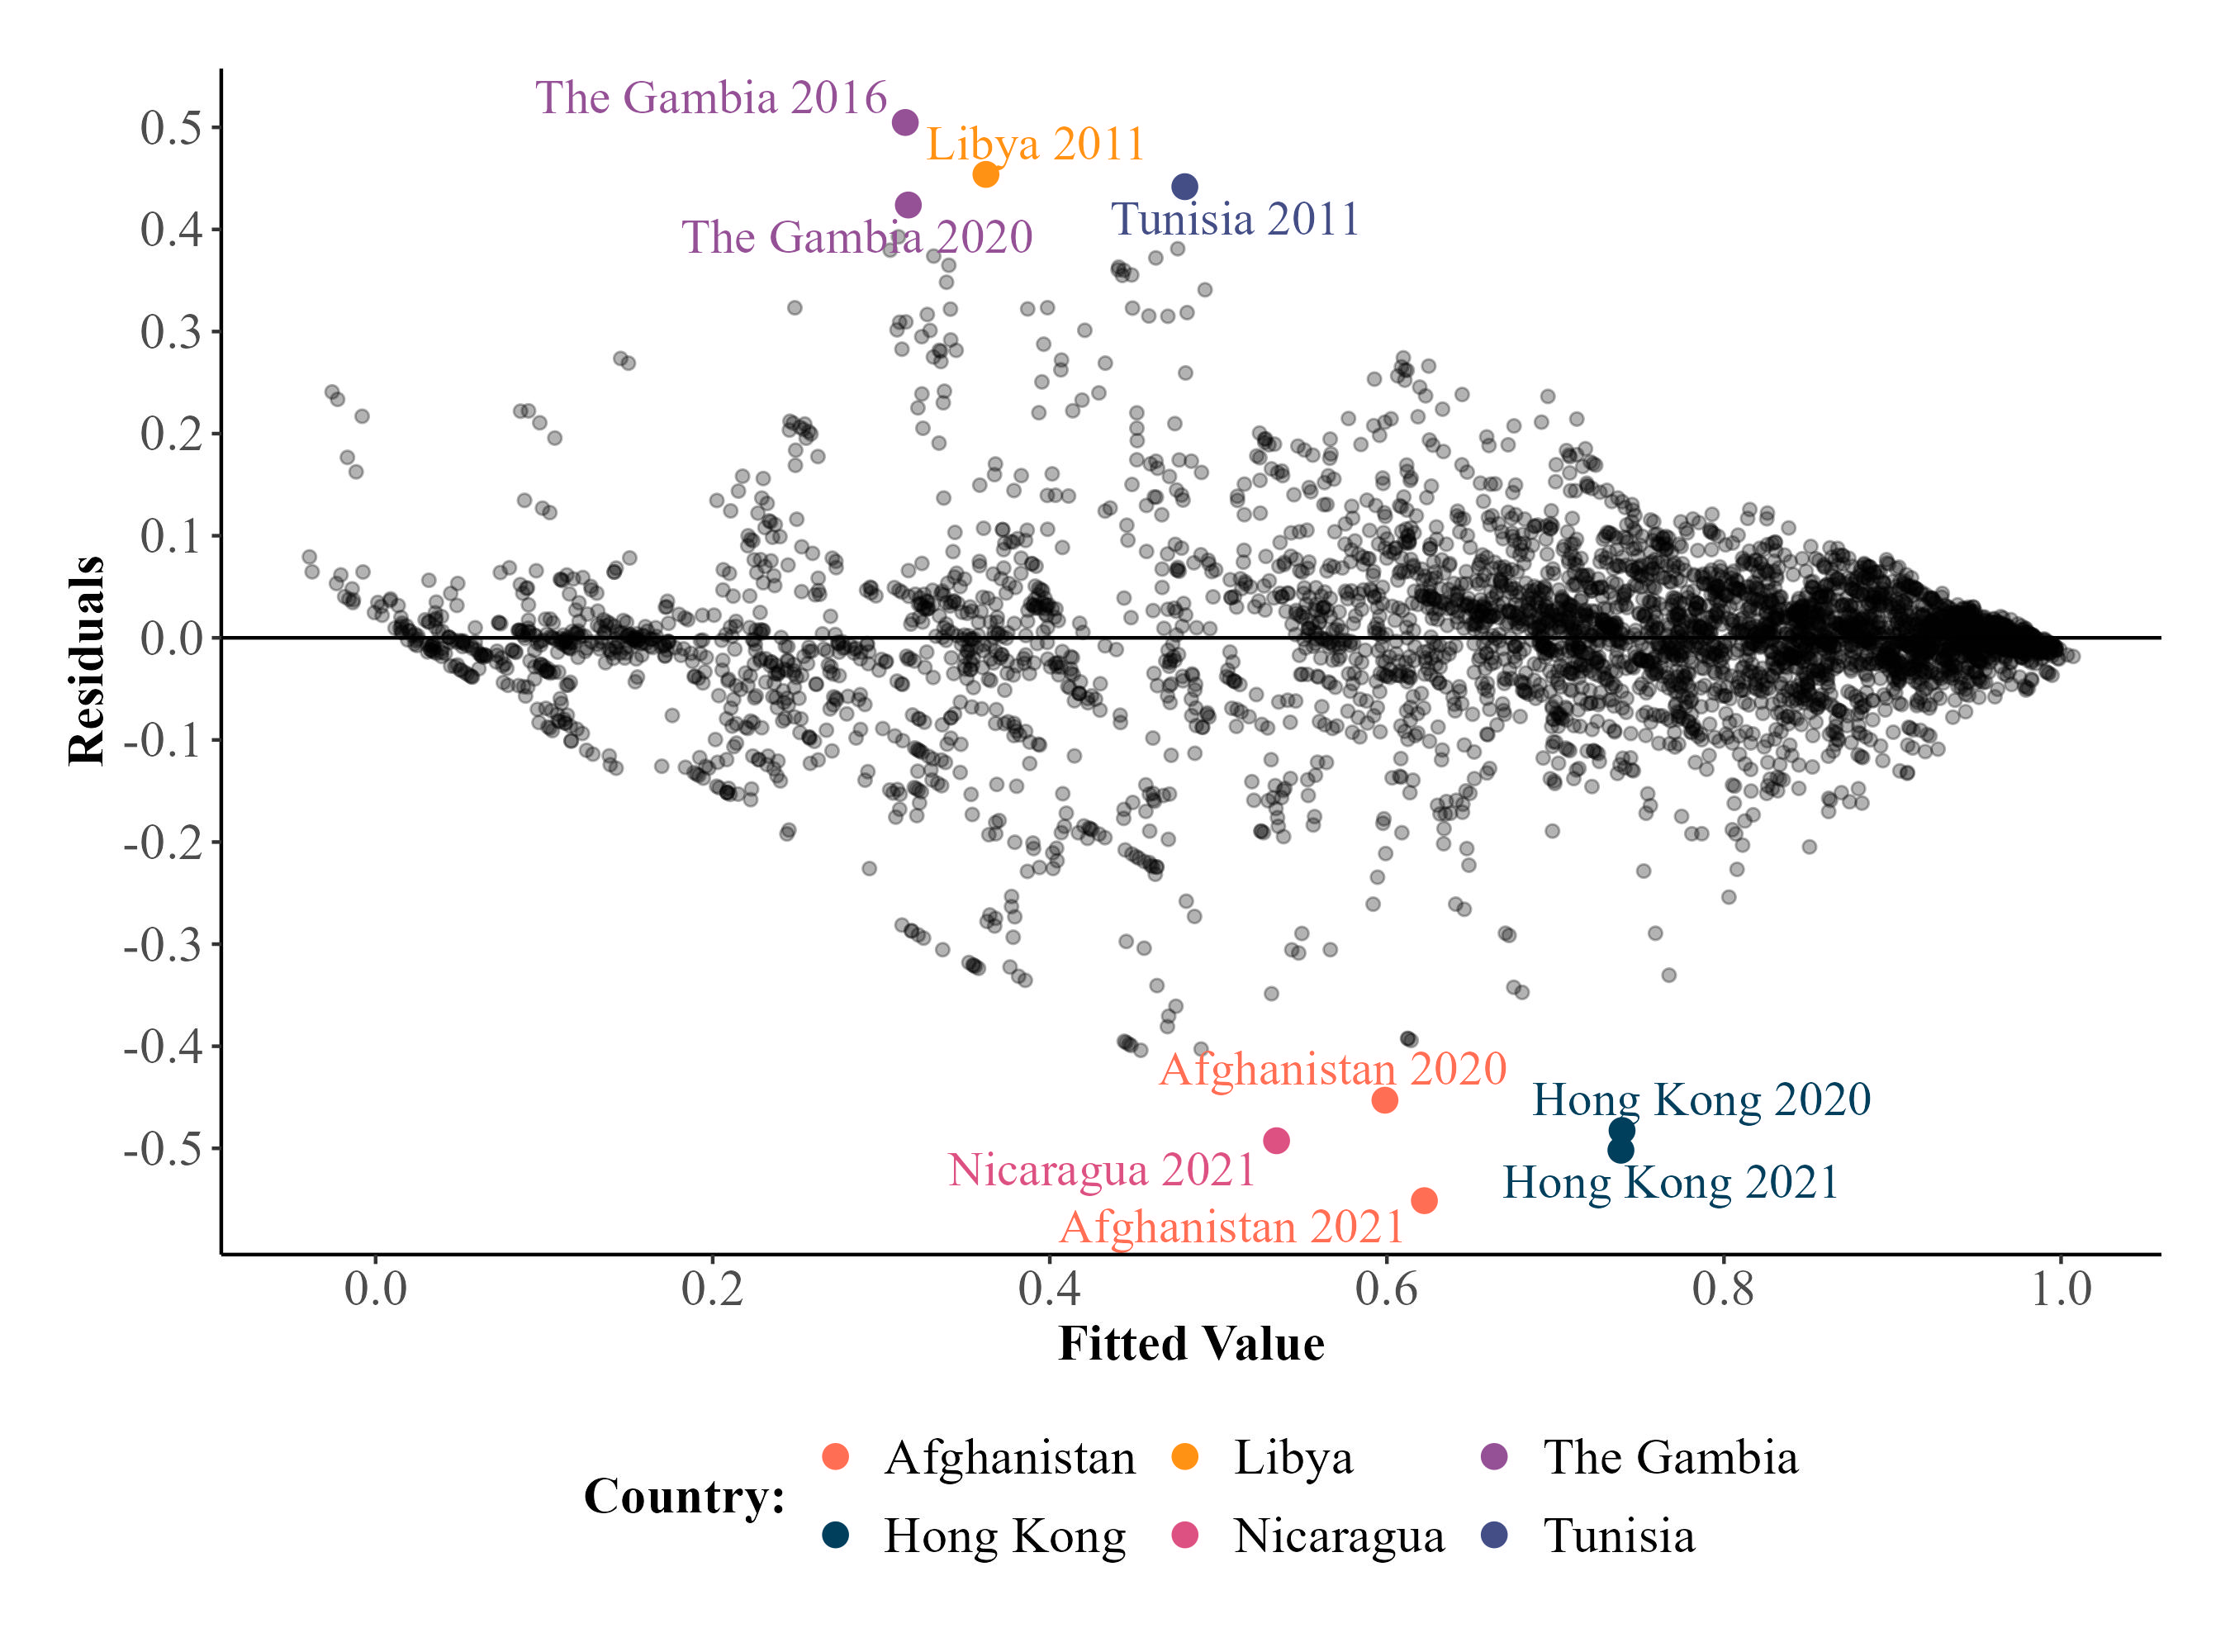
\includegraphics[width=.9\linewidth]{graphics/residuals.jpeg}
    \caption{Residual plot for Model 2.5}
    \label{fig:residuals}
\end{figure}

\chapter{Notes} \label{apn:notes}
\lettrine{T}{his part of the appendix} includes some notes on the figures, as well as some descriptive data which was unnecessary to include in the main part of the thesis. I include this in the appendix so that everything I have done is reproducible.

\section{Countries} \label{sec:countries}
I first include a list over all the countries featured in the regression. I have information for the two main variables (freedom of expression and linkages to China) for almost every year between 1994. There are of course some country that have split up over this period and these are counted as separate countries. For the freedom of expression variable I have data up until 2024, as the new V-Dem data \citep{coppedge_v-dem_2025} was released in March. The table also accounts for missingness on the other variables. E.g., I do not have data on natural resources rents for Afghanistan between 1994 and 2001, and I do not have aid data for 2023.


{\fontsize{8pt}{8pt}\selectfont\tabcolsep=2pt\centering  % hold it local
\begin{longtable}{lcccccc}
\caption{Country}
\label{tab:country} \\ % This linebreak is what makes the caption work! 
\toprule
Country & Start year & End year\textsuperscript{1} & NA GDP & NA rents\textsuperscript{2} & NA aid & NA West\\
\midrule
Afghanistan & 1994 & 2023 &  & 1994-2001 & 2023 & \\
Albania & 1994 & 2023 &  &  &  & \\
Algeria & 1994 & 2023 &  &  &  & \\
Angola & 1994 & 2023 &  &  &  & \\
Argentina & 1994 & 2023 &  &  &  & \\
\addlinespace
Armenia & 1994 & 2023 &  &  &  & \\
Australia & 1994 & 2023 &  &  &  & \\
Austria & 1994 & 2023 &  &  &  & \\
Azerbaijan & 1994 & 2023 &  &  &  & \\
Bahrain & 1994 & 2023 &  &  &  & \\
\addlinespace
Bangladesh & 1994 & 2023 &  &  &  & \\
Barbados & 1994 & 2023 &  &  &  & \\
Belarus & 1994 & 2023 &  &  &  & \\
Belgium & 1994 & 2023 &  &  &  & \\
Benin & 1994 & 2023 &  &  &  & \\
\addlinespace
Bhutan & 1994 & 2023 &  &  & 2023 & \\
Bolivia & 1994 & 2023 &  &  &  & \\
Bosnia and Herzegovina & 1994 & 2023 &  &  &  & \\
Botswana & 1994 & 2023 &  &  &  & \\
Brazil & 1994 & 2023 &  &  &  & \\
\addlinespace
Bulgaria & 1994 & 2023 &  &  &  & \\
Burkina Faso & 1994 & 2023 &  &  &  & \\
Burma/Myanmar & 1994 & 2023 &  &  &  & \\
Burundi & 1994 & 2023 &  &  &  & \\
Cambodia & 1994 & 2023 &  &  &  & \\
\addlinespace
Cameroon & 1994 & 2023 &  &  &  & \\
Canada & 1994 & 2023 &  &  &  & \\
Cape Verde & 1994 & 2023 &  &  &  & \\
Central African Republic & 1994 & 2023 &  &  &  & \\
Chad & 1994 & 2023 &  &  &  & \\
\addlinespace
Chile & 1994 & 2023 &  &  & 2018 & \\
Colombia & 1994 & 2023 &  &  &  & \\
Comoros & 1994 & 2023 &  &  &  & \\
Costa Rica & 1994 & 2023 &  &  &  & \\
Croatia & 1994 & 2023 &  & 1994 &  & \\
\addlinespace
Cuba & 1994 & 2023 & 2023 & 2021 & 2023 & \\
Cyprus & 1994 & 2023 &  &  &  & \\
Czechia & 1994 & 2023 &  &  &  & \\
Democratic Republic of the Congo & 1994 & 2023 &  &  &  & \\
Denmark & 1994 & 2023 &  &  &  & \\
\addlinespace
Djibouti & 1994 & 2023 &  &  &  & \\
Dominican Republic & 1994 & 2023 &  &  &  & \\
Ecuador & 1994 & 2023 &  &  &  & \\
Egypt & 1994 & 2023 &  &  &  & \\
El Salvador & 1994 & 2023 &  &  &  & \\
\addlinespace
Equatorial Guinea & 1994 & 2023 &  & 2001-2004 &  & \\
Eritrea & 1994 & 2023 & 2023 & 2012- & 2023 & \\
Estonia & 1994 & 2023 &  & 1994 &  & \\
Eswatini & 1994 & 2023 &  &  &  & \\
Ethiopia & 1994 & 2023 &  &  &  & \\
\addlinespace
Fiji & 1994 & 2023 &  &  &  & \\
Finland & 1994 & 2023 &  &  &  & \\
France & 1994 & 2023 &  &  &  & \\
Gabon & 1994 & 2023 &  &  &  & \\
Georgia & 1994 & 2023 &  &  &  & \\
\addlinespace
Germany & 1994 & 2023 &  &  &  & \\
Ghana & 1994 & 2023 &  &  &  & \\
Greece & 1994 & 2023 &  &  &  & \\
Guatemala & 1994 & 2023 &  &  &  & \\
Guinea & 1994 & 2023 &  &  &  & \\
\addlinespace
Guinea-Bissau & 1994 & 2023 &  &  &  & \\
Guyana & 1994 & 2023 &  &  &  & \\
Haiti & 1994 & 2023 &  &  &  & \\
Honduras & 1994 & 2023 &  &  &  & \\
Hong Kong & 1997 & 2023 &  &  &  & 1994-1996\\
\addlinespace
Hungary & 1994 & 2023 &  &  &  & \\
Iceland & 1994 & 2023 &  &  &  & \\
India & 1994 & 2023 &  &  &  & \\
Indonesia & 1994 & 2023 &  &  &  & \\
Iran & 1994 & 2023 &  &  &  & \\
\addlinespace
Iraq & 1994 & 2023 &  &  &  & \\
Ireland & 1994 & 2023 &  &  &  & \\
Israel & 1994 & 2023 &  & 1994 &  & \\
Italy & 1994 & 2023 &  &  &  & \\
Ivory Coast & 1994 & 2023 &  &  &  & \\
\addlinespace
Jamaica & 1994 & 2023 &  &  &  & \\
Japan & 1994 & 2023 &  &  &  & \\
Jordan & 1994 & 2023 &  &  &  & \\
Kazakhstan & 1994 & 2023 &  &  &  & \\
Kenya & 1994 & 2023 &  &  &  & \\
\addlinespace
Kosovo & 2008 & 2023 &  & 1999-2007 & 1999-2008 & 1999-2007\\
Kuwait & 1994 & 2023 &  & 2021 &  & \\
Kyrgyzstan & 1994 & 2023 &  &  &  & \\
Laos & 1994 & 2023 &  &  &  & \\
Latvia & 1994 & 2023 &  & 1994 &  & \\
\addlinespace
Lebanon & 1994 & 2023 &  &  & 2023 & \\
Lesotho & 1994 & 2023 &  &  &  & \\
Liberia & 1994 & 2023 &  & 1994-1999 &  & \\
Libya & 1994 & 2023 &  &  & 2000-2004 & \\
Lithuania & 1994 & 2023 &  & 1994 &  & \\
\addlinespace
Luxembourg & 1994 & 2023 &  &  &  & \\
Madagascar & 1994 & 2023 &  &  &  & \\
Malawi & 1994 & 2023 &  &  &  & \\
Malaysia & 1994 & 2023 &  &  &  & \\
Maldives & 1994 & 2023 &  &  &  & \\
\addlinespace
Mali & 1994 & 2023 &  &  &  & \\
Malta & 1994 & 2023 &  &  &  & \\
Mauritania & 1994 & 2023 &  &  &  & \\
Mauritius & 1994 & 2023 &  &  &  & \\
Mexico & 1994 & 2023 &  &  &  & \\
\addlinespace
Moldova & 1994 & 2023 &  & 1994 & 1994-1996 & \\
Mongolia & 1994 & 2023 &  &  &  & \\
Montenegro & 2006 & 2023 &  & 1998-1999 & 1998-2002 & 1998-2005\\
Morocco & 1994 & 2023 &  &  &  & \\
Mozambique & 1994 & 2023 &  &  &  & \\
\addlinespace
Namibia & 1994 & 2023 &  &  &  & \\
Nepal & 1994 & 2023 &  &  &  & \\
Netherlands & 1994 & 2023 &  &  &  & \\
New Zealand & 1994 & 2023 &  &  &  & \\
Nicaragua & 1994 & 2023 &  &  &  & \\
\addlinespace
Niger & 1994 & 2023 &  &  &  & \\
Nigeria & 1994 & 2023 &  &  &  & \\
North Korea & 1994 & 2023 & 2023 & Not included & 2023 & \\
North Macedonia & 1994 & 2023 &  &  &  & \\
Norway & 1994 & 2023 &  &  &  & \\
\addlinespace
Oman & 1994 & 2023 &  &  &  & \\
Pakistan & 1994 & 2023 &  &  &  & \\
Panama & 1994 & 2023 &  &  &  & \\
Papua New Guinea & 1994 & 2023 &  &  &  & \\
Paraguay & 1994 & 2023 &  &  &  & \\
\addlinespace
Peru & 1994 & 2023 &  &  &  & \\
Philippines & 1994 & 2023 &  &  &  & \\
Poland & 1994 & 2023 &  &  &  & \\
Portugal & 1994 & 2023 &  &  &  & \\
Qatar & 1994 & 2023 &  &  &  & \\
\addlinespace
Republic of the Congo & 1994 & 2023 &  &  &  & \\
Romania & 1994 & 2023 &  &  &  & \\
Russia & 1994 & 2023 &  &  &  & \\
Rwanda & 1994 & 2023 &  &  &  & \\
Sao Tome and Principe & 1994 & 2023 &  & 1994-2000 &  & \\
\addlinespace
Saudi Arabia & 1994 & 2023 &  &  &  & \\
Senegal & 1994 & 2023 &  &  &  & \\
Serbia & 2006 & 2023 &  & 1994 &  & 1994-2005\\
Seychelles & 1994 & 2023 &  &  &  & \\
Sierra Leone & 1994 & 2023 &  &  &  & \\
\addlinespace
Singapore & 1994 & 2023 &  &  &  & \\
Slovakia & 1994 & 2023 &  &  &  & \\
Slovenia & 1994 & 2023 &  & 1994 &  & \\
Solomon Islands & 1994 & 2023 &  &  &  & \\
Somalia & 1994 & 2023 &  & 1994-2012 &  & \\
\addlinespace
South Africa & 1994 & 2023 &  &  &  & \\
South Korea & 1994 & 2023 &  &  &  & \\
South Sudan & 2011 & 2023 &  & 2016- & 2023 & \\
Spain & 1994 & 2023 &  &  &  & \\
Sri Lanka & 1994 & 2023 &  &  &  & \\
\addlinespace
Sudan & 1994 & 2023 &  &  &  & \\
Suriname & 1994 & 2023 &  &  &  & \\
Sweden & 1994 & 2023 &  &  &  & \\
Switzerland & 1994 & 2023 &  &  &  & \\
Syria & 1994 & 2023 & 2023 & 2021 & 2023 & \\
\addlinespace
Taiwan & 1994 & 2023 &  & Not included &  & \\
Tajikistan & 1994 & 2023 &  &  &  & \\
Tanzania & 1994 & 2023 &  &  &  & \\
Thailand & 1994 & 2023 &  &  &  & \\
The Gambia & 1994 & 2023 &  &  &  & \\
\addlinespace
Timor-Leste & 2002 & 2023 &  & 1994-1999 and 2004-2014 &  & 1994-2001\\
Togo & 1994 & 2023 &  &  &  & \\
Trinidad and Tobago & 1994 & 2023 &  &  &  & \\
Tunisia & 1994 & 2023 &  &  &  & \\
Turkmenistan & 1994 & 2023 &  & 2020- &  & \\
\addlinespace
Türkiye & 1994 & 2023 &  &  &  & \\
Uganda & 1994 & 2023 &  &  &  & \\
Ukraine & 1994 & 2023 &  &  &  & \\
United Arab Emirates & 1994 & 2023 &  &  &  & \\
United Kingdom & 1994 & 2023 &  &  &  & \\
\addlinespace
United States of America & 1994 & 2023 &  &  &  & \\
Uruguay & 1994 & 2023 &  &  &  & \\
Uzbekistan & 1994 & 2023 &  &  &  & \\
Vanuatu & 1994 & 2023 &  &  &  & \\
Venezuela & 1994 & 2023 &  & 2015- & 2023 & \\
\addlinespace
Vietnam & 1994 & 2023 &  &  &  & \\
Yemen & 1994 & 2023 &  & 1994-2001 & 2023 & \\
Zambia & 1994 & 2023 &  &  &  & \\
Zimbabwe & 1994 & 2023 &  &  &  & \\
\bottomrule
\multicolumn{7}{l}{\rule{0pt}{1em}\textsuperscript{1} I have data on the freedom variable for all countries up until 2024.} \\ 
\multicolumn{7}{l}{\rule{0pt}{1em}\textsuperscript{2} Natural resources rents only has data from 1994-2021, missing data indicates missing variables other than 2022-2023} \\
\end{longtable}
}

\section{The West}
I have defined the West as being as being countries with a strong tradition of democratic government going back to to at least the 1990s. From Europe I have included the EU 27, EFTA, Andorra, San Marino, and the United Kingdom. From North America I have included the Canada and the United States of America (USA). From Oceania I have included Australia and New Zealand. From East Asia I include Japan, South Korea, and Taiwan. Finally from the Middle East I include Israel. I admit that countries like Hungary and Israel are dubious in some respects, but Hungary is a part of one of the biggest democracy promoting organisations in the world: the EU, and Israel has mostly been democratic, even if it more and more resembles an apartheid state.

\begin{table}[H]
    \centering
    \caption{Countries included in the definition of the `West'}
    \label{tab:west}
    \vspace{0.5em}
    \begin{tabular}{lllll}
    \toprule
         Europe & East Asia & North America & Oceania & Middle East \\ 
    \midrule
         Andorra & Japan & Canada & Australia & Israel \\
         Austria & South Korea & USA & New Zealand & \\
         Belgium & Taiwan & & & \\
         Bulgaria & & & & \\
         Croatia & & & & \\
         Cyprus & & & & \\
         Czech Republic & & & & \\
         Denmark & & & & \\
         Estonia & & & & \\
         Finland & & & & \\
         France & & & & \\
         Germany & & & & \\ 
         Greece & & & & \\
         Hungary & & & & \\ 
         Iceland & & & & \\ 
         Ireland & & & & \\
         Italy & & & & \\
         Latvia & & & & \\ 
         Liechtenstein & & & & \\ 
         Lithuania & & & & \\
         Luxembourg & & & & \\ 
         Malta & & & & \\
         Netherlands & & & & \\
         Norway & & & & \\ 
         Poland & & & & \\
         Portugal & & & & \\
         Romania & & & & \\
         San Marino & & & & \\
         Slovakia & & & & \\ 
         Slovenia & & & & \\
         Spain & & & & \\ 
         Sweden & & & & \\
         Switzerland & & & & \\
         UK & & & & \\
    \bottomrule
    \end{tabular}
\end{table}

\section{Figures}
Here follows some notes on the figures included in the thesis. I have had to make certain choices and I will justify them in this part of the appendix.  

\subsection{Figure \ref{fig:declining}: declining indicators}
Figure \ref{fig:declining} shows, according to the V-Dem institutes data, the variables that have declined most over a ten-year period. This is calculated from the V-Dem data, and is featured in V-Dem's annual democracy report \citep[p. 17]{nord_democracy_2025}. The figure I am using is taken directly from this report, as the methodology for creating it is unclear.

\subsection{Figure \ref{fig:autocratisation}: autocratisation}
This figure is based on V-Dem's Electoral Democracy Index and shows the development of democracy from 1900. Normally the separation between democracy and autocracy goes at 0.5, with autocracies being less than 0.5 and democracies greater. This can easily be used for a present definition, however, as the historical level of democracy is very low, I have decided to use a threshold value of 0.3. This better shows the decline in democracy in the two previous waves. We are also not interested here in the number of democracies, but rather the change in democracy scores, and this is an indicator of this.

\subsection{Figure \ref{fig:link-china}: linkages to China}
For this figure I have made some important decisions that impact some of the results if done to other specifications. The first problem I had, was that some of the countries did not have numbers for 1994. This problem mainly occurs as an artifact of countries splitting up. There are four major countries affected by this: Kosovo, Montenegro, Serbia, and South Sudan. To include them, I decided to use their pre-independence counterpart as the 1994 value. This probably makes the values for 1994 artificially high, leading them to getting a lower score than would else have been the case. This is highly likely in the case of Serbia. The second thing to note is the definition of the size of the changes. I have arbitrarily defined them, based on what is normal in the same data. I have made the following distinctions: Higher than 0.2 change in linkages equals a very strong change. Change between 0.2 and 0.08 i define as a strong change. Change between 0.08 and 0.03 I define as change, and everything between 0 and 0.03 I define as `no or small change.'

\subsection{Figure \ref{fig:west}: linkages to the West}
The problems for this figure mirrors those in Figure \ref{fig:link-china} so I will be a bit more brief here. I have made the same adjustments for the countries, however since the linkage variable for the West is aggregated, I use different values for the change-intervals. Higher than 0.25 is a very strong change. Changes between 0.15 and 0.25 is defined as a strong change, while values between 0.05 and 0.15 I define as a normal change. Any change smaller than this I have defined as `no or small change.' 

\subsection{Figure \ref{fig:scp}: single country plots}
For the single country plots I chose countries based on Table \ref{tab:change}. Unlike in the maps, I have not combined countries that have split up. I have done this because the values of the countries that are measured against a larger version of themselves would be artificial. Since both variables are measured between 0 and 1, I have decided to plot them with a single y-axis. 
%TC:endignore 
\end{document}
